\documentclass[times, utf8, zavrsni, numeric]{fer}
\usepackage{booktabs}
\usepackage{lipsum}
\usepackage{float}
\usepackage{pdfpages}
\usepackage{graphicx} 
\usepackage{hyperref}
\usepackage{svg}
\usepackage[linesnumbered,ruled,vlined]{algorithm2e}
\usepackage{chngcntr}
\usepackage{longtable}
\usepackage{array}
\usepackage{amsmath}

\graphicspath{ {./images/} }

\def\labelitemi{$\cdot$}

\counterwithin{algocf}{chapter}

\begin{document}

\thesisnumber{496}

\title{Optimization of Hyperheuristics for Online Scheduling Problems}

\author{Mihael Miličević}

\maketitle

\includepdf[]{izvornik.pdf}

\zahvala{
    
To my mentor, prof. Jakobović, for your support and guidance. To my friends, for your companionship and encouragement. To my parents, for your unconditional love and sacrifices.

Thank you all.

}

\tableofcontents

\chapter{Introduction}
\label{sec:introduction}
Scheduling is the decision-making process which solves the problems of allocating limited resources to tasks over a given time. The model of scheduling used in this thesis has the following setup - a system contains $m$ machines which are organized in some way, a total $k$ jobs need to be processed on the system, and the scheduling in this context entails deciding, at every moment, which job is being processed on which machine, in order to optimize some criteria. 

Scheduling problems are interesting optimization problems because they are hard to solve. For most non-trivial setups, an exhaustive approach is not applicable. Instead, heuristic approaches are used. In this thesis, our goal will be to solve online scheduling problems, where the exact sequence of jobs which needs to be processed is not known in advance, and instead the information about a job becomes known only when it enters the system. We will solve such problems using hyperheuristics, which are heuristic approaches used to find good ways to solve a problem.

Chapter \ref{sec:theoretical_background} of this thesis covers the theoretical background required for solving online scheduling problems. Chapter \ref{sec:topology_model} introduces the hierarchical topology model, which is a versatile model capable of representing a wide range of scheduling systems. Chapter \ref{sec:events_model} introduces the events model, which will be used for modelling complex behaviors such as machine breakdowns, preemptions, prerequisites, machine buffers with a limited size, setups and batch processing. Chapter \ref{sec:evaluation_model} introduces the evaluation model for the hierarchical topology representation. Chapter \ref{sec:optimization_model} covers the concepts which allow building modular optimization algorithms, and which will be used in all optimization algorithms throughout this thesis. Chapter \ref{sec:offline_scheduling_model} explains how the hierarchical topology representation can be used for solving offline scheduling problems. In such problems, the data about jobs is completely known in advance, which in theory makes the optimization easier to perform. While offline scheduling is not a central concept for this thesis, understanding it will be a great stepping stone to understanding online scheduling. Chapter \ref{sec:online_scheduling_model} explains how the hierarchical topology representation can be used for solving online scheduling problems. Chapter \ref{sec:experiments_and_results} covers several online scheduling case studies, and includes hyperparameter tuning, experimental setups, results and examples of generated heuristics. On the surface, these case studies encompass problems which are quite different one from another. But they will all be solved using the same scheduling framework, as a testament to the versatility and complexity of the hierarchical topology representation. Finally, chapter \ref{sec:conclusion} covers the conclusion of the thesis.

\chapter{Theoretical background}
\label{sec:theoretical_background}

In this chapter, we will go over the theoretical background topics which are necessary to understand this thesis. These topics include mathematical optimization, heuristic optimization and scheduling theory.

\section{Optimization}
\label{sec:optimization}

\subsection{Mathematical formulation}
\label{sec:mathematical_formulation}
Optimization is the minimization or maximization of a function $f(x)$ subject to constraints $c_i(x) = 0, c_j(x) \ge 0$ on its variables $x \in \mathbb{R}^n$ \citep{nocedal2006numericaloptimization}. Minimization and maximization pose equivalent optimization problems, as minimizing $f(x)$ is the same as maximizing $-f(x)$. In this thesis, we will be solving minimization problems.

\subsection{Continuous and discrete optimization}
\label{sec:continuous_and_discrete_optimization}
In continuous optimization, the feasible set of solutions is uncountably infinite, such as the set of real numbers. These problems are usually easier to solve because of the smoothness of the optimization function, which makes it possible to deduce information about the function's behavior at all points close to a point $x$. On the other hand, in discrete optimization, the feasible set of solutions can be the set of integers, or of a more complex structure, such as permutations of an ordered set. These problems are typically harder to solve, because the behavior of the function can significantly change as we move from one feasible solution to another. In this thesis, we will be solving discrete optimization problems.

\subsection{Constrained and unconstrained optimization}
\label{sec:constrained_and_unconstrained_optimization}
If an optimization problem has at least one constraint $c_i(x) = 0$ or $c_i(x) \ge 0$, then the problem can be categorized as a constrained optimization problem. If the problem has no constraints, then it can be categorized as an unconstrained optimization problems. Constrained optimization problems are typically harder to solve, as the constraints can complicate the search process. In this thesis, we will be solving constrained problems.

\subsection{Global and local optimization}
\label{sec:global_and_local_optimization}
In local optimization problems, the goal is to find a solution that is better than all other feasible solutions which are close to the solution in the search space. On the other hand, in global optimization problems, the goal is to find the best solution among all feasible solutions. Global optimization problems are typically much harder to solve, especially if the optimization function is highly nonlinear, having many local optima. In this thesis, we will be solving global optimization problems.

\subsection{Deterministic and stochastic optimization}
\label{sec:deterministic_and_stochastic_optimization}
The algorithm used to search for a solution can be deterministic or stochastic. If it is deterministic, it will always yield the same results on a particular problem. On the other hand, if the algorithm is stochastic, it will use a random number generator when searching for a solution, and this means that different runs of the same algorithm will yield different results. In this thesis, we will be doing stochastic optimization.

\subsection{Example: The travelling salesman problem}
\label{sec:the_travelling_salesman_problem}
To demonstrate the types of problems we will solve in this thesis, we will go over the travelling salesman problem. The setup for this problem is that a salesman starts his journey in a city, has to visit every city exactly once, and has to return to the starting city. The goal is to minimize the distance that the traveller makes in his journey. In terms of graph theory, the goal is to find the shortest Hamiltonian cycle in the graph comprised of all the cities that the salesman has to visit. This problem is an NP-complete problem \citep{sipser2012computation}, meaning that no algorithm for solving it which runs in polynomial time is known.

The problem is discrete, as every permutation of the sets of cities represents one feasible solution. It is constrained, because the traveller can visit every city exactly once and return to the starting city at the end. The goal is to find the shortest Hamiltonian cycle, so this problem is global. Finally, the problem could be solved both deterministically and stochastically. A deterministic algorithm would go over all possible permutations of the set of cities to find the shortest cycle. While this algorithm would find the global optimum, the problem is intractable, meaning that after a certain point in the size of the problem, where size is measured in the number of cities that the traveller needs to visit, it would take unreasonably long time to terminate the algorithm. Instead, stochastic algorithms are used for solving larger problems.

In Figure \ref{fig:tsp}, a simple travelling salesman problem is demonstrated. The left image shows a grid of cities, and the right image shows the shortest Hamiltonian cycle in the grid. This figure, and all the subsequent figures in this thesis, were created using the draw.io software \citep{drawio}.

\begin{figure}[!htbp]
	\centering
	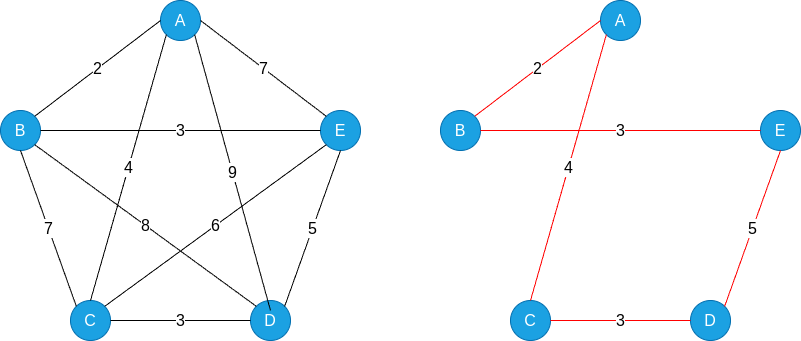
\includegraphics[scale=0.25]{../images/TSP.png}
	\caption{The travelling salesman problem}
    \label{fig:tsp}
\end{figure}
\section{Heuristic optimization}
\label{sec:heuristic_optimization}

\subsection{Heuristics}
\label{sec:heuristics}
Heuristics are techniques based on experience used for solving a specific problem. They are expected to provide a satisfactory solution in a reasonable computation time, but they do not guarantee to find the optimal solution. They can be based on domain knowledge, and they can include criteria such as a rule of thumb, an educated guess, an intuitive judgement or common sense \citep{swamy2016search}.

\subsection{Metaheuristics}
\label{sec:metaheuristics}
Metaheuristics are high-level heuristics that guide the design of problem-specific heuristics \citep{swamy2016search}. They are used to find, tune or select heuristics that may be used to find a solution to the problem. They can search over a large set of feasible solutions, and thus they can usually yield better results than just problem-specific heuristics. The two main types of metaheuristics are solution-based and population-based metaheuristics. The former operate on a single solution which is changed during the course of the algorithm, while the latter maintain a population of solutions from which the best one is chosen when the algorithm terminates.

\subsection{Hyperheuristics}
\label{sec:hyperheuristics}
Hyperheuristics are heuristics used for searching the space of problem-specific heuristics \citep{Chakhlevitch2008}. Similar to metaheuristics, they also operate on a level above heuristics, but the difference is that metaheuristics search a space of solutions. A key characteristic of hyperheuristics is that they don't search for a good solution to the problem, instead, they search for a good method to solve the problem. In this thesis, we will use metaheuristics to search the space of problem-specific heuristics, which is an approach that the authors in \citep{Chakhlevitch2008} called metaheuristics-based hyperheuristics.
\section{Scheduling}
\label{sec:scheduling}

\subsection{Model of scheduling}
\label{sec:model_of_scheduling}
Scheduling is a decision-making process used to allocate resources to tasks over a given time, with the goal of optimizing one or more objectives \citep{pinedo2016scheduling}. This model can be applied to a many different domains. For example, the resources can represent machines in a workshop, and the tasks can be operations in a production process. In another example, the resources can be crews at a construction site, and tasks can be stages in a construction process. In one more example, the resources can be processing units in a computing environment, and the tasks can be the executions of computer programs. The objectives can be the minimization of the completion time of the last task, or the minimization of the number of tasks completed after their deadline, or any other criteria used for evaluating the schedule.

Following the notation described in \citep{pinedo2016scheduling}, a scheduling problem can be described by a triplet $\alpha | \beta | \gamma$. The field $\alpha$ describes the machine environment. The field $\beta$ describes processing characteristics and constraints. The field $\gamma$ describes the objective to be optimized. All these fields and their possible values will be described in detail in chapters \hyperref[sec:topology_model]{3}, \hyperref[sec:events_model]{4} and \hyperref[sec:evaluation_model]{5} respectively, when we discuss the system proposed in this thesis, which is an implementation of this model of scheduling.

To illustrate the inherent complexity of solving a scheduling problem, we will consider the problem $1|r_j|L_{max}$. In this problem, the $\alpha$ parameter is $1$, which means the system contains a single machine. The $\beta$ parameter is $r_j$, which means that the job $j$ becomes available at time $r_j$, where $r$ is the symbol for release date. The $\gamma$ is an objective function called maximum lateness function, where the maximum of $L_j = C_j - d_j$ for every job $j$ is chosen, $C_j$ is the time that the job exits the system, and $d_j$ is the due time when the job was expected to exit the system. This problem is NP-hard, as proven in \citep{pinedo2016scheduling}. Compared to problems we will use for experiments in chapter \hyperref[sec:experiments_and_results]{4}, it is a relatively simple problem, but nevertheless, in terms of the computation theory, it is a hard problem. Due to the complexity which arises when dealing with scheduling, heuristic optimization approaches play a central role in scheduling optimization problems.

\subsection{Online and offline scheduling}
\label{sec:offline_and_online_scheduling}
Scheduling problems can be categorized in two main categories, offline and online scheduling. In an offline scheduling problem, all problem data is known prior to solving the problem. In this context, the term problem data refers to information about the number of tasks, and the characteristics of each task. In an online scheduling problem, the problem data is not known in advance, and instead it becomes available only when the system is executing. The number of tasks may not be known in advance, and the characteristics of each task become available only when the task becomes active and available to solve \citep{pinedo2016scheduling}. In this thesis, we will discuss both offline and online scheduling.

\subsection{Representations for scheduling problems}
\label{sec:representations_for_scheduling_problems}
There are several types of machine environments which can be expressed using the model of machines and jobs, and for each of them, distinct representations have been proposed \citep{werner2013survey}. For flow shops, where each job has the same route through the system, a permutation of jobs as representation of the solution has been proposed. For job shops, where each job has its own route, a similar approach has been used, with each machine having its own separate permutation. Finally, for open shops, where no limitations are imposed on job routes, several representations have been proposed, with one of them being a string encoding for the schedule construction.

There are also several systems which can be thought of as implementations of this model. One of them is Lekin \citep{lekin}, developed as an educational tool, and used for offline scheduling across several workspace environments: single machine, parallel machines, flow shop, flexible flow shop, job shop and flexible job shop.

In the next chapter, a new system of representation will be proposed. This system is a faithful implementation of the model of machines and jobs, and it supports both offline and online scheduling.

\chapter{Topology model}
\label{sec:topology_model}

In this chapter, we will describe the first component of the hierarchical topology representation, which is its topology model.

\section{Topology building blocks}
\label{sec:topology_building_blocks}
The representation system proposed in this thesis is hierarchical. This means that the system of machines can be represented using a tree structure.

The leaves in the tree are machines. Each machine has its buffer which contains jobs waiting for processing. Whenever the machine is free, a job is chosen from the buffer and put on the machine for processing.

The inner nodes in the tree are groups. Every group has at least one child component, and these components can be either machines or groups. This simple recursive rule allows building of arbitrarily complex systems of machines. Throughout the remainder of this thesis, we will refer to a system of machines and its inner connections as a topology. 

To reiterate, topologies correspond to tree structures. Another data structure which is very important for this system is directed acyclic graphs (DAGs). DAGs are used to store the possible paths which a job can take when going through the topology.

Every group can be thought of as an abstract machine. When a job enters the group, it will be processed on it, the same as it would be on a machine, but this processing will be instant and then the job will be directed to the next component on its path. There are several types of groups. 

\subsection{Serial group}

The first group type is the serial group. The components of this group are ordered. When a job enters this group, it is directed to its first component, and then second, all the way to the last one. Figure \ref{fig:serial_group} shows a serial group topology on the left, and the corresponding paths DAG on the right. Serial group nodes are named S, while machines are named M.

\begin{figure}[!htbp]
	\centering
	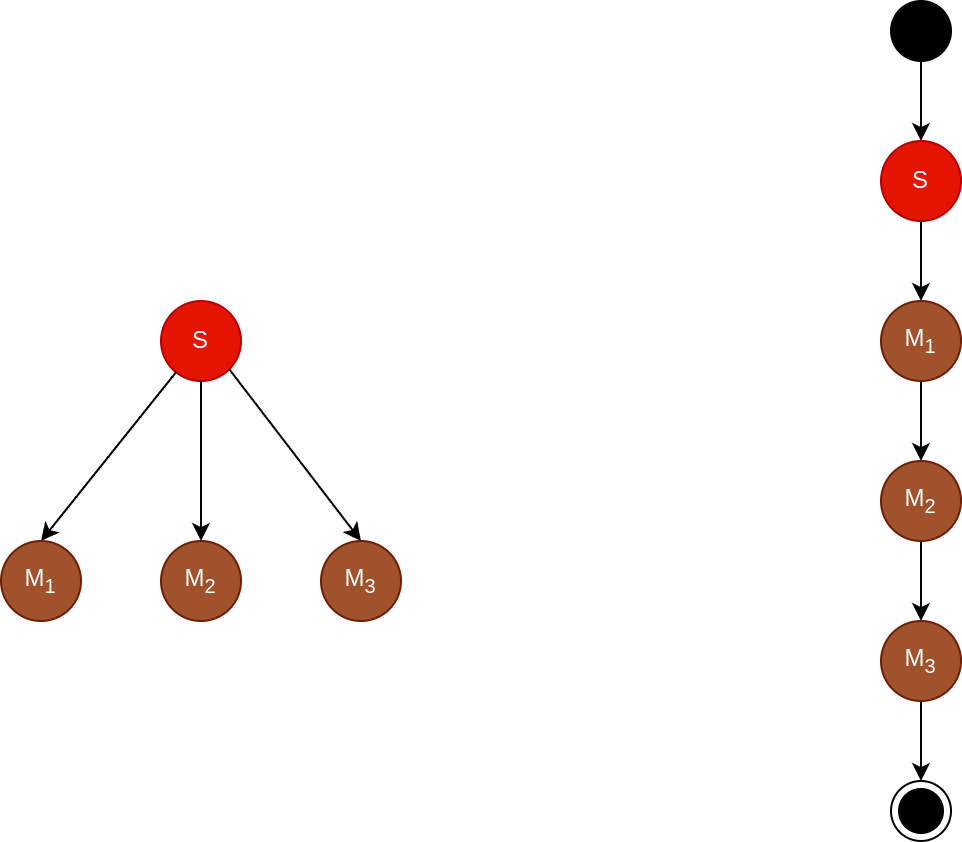
\includegraphics[scale=0.3]{../images/serial_group.png}
	\caption{Serial group - topology and paths}
    \label{fig:serial_group}
\end{figure}

\subsection{Parallel group}

The second group type is parallel group. This group performs a branching over its components. When a job enters this group, it is directed to one of its components, and the job will only be processed in that component. Figure \ref{fig:parallel_group} shows a parallel group topology on the left, and the corresponding paths DAG on the right. Parallel group nodes are named P.

\begin{figure}[!htbp]
	\centering
	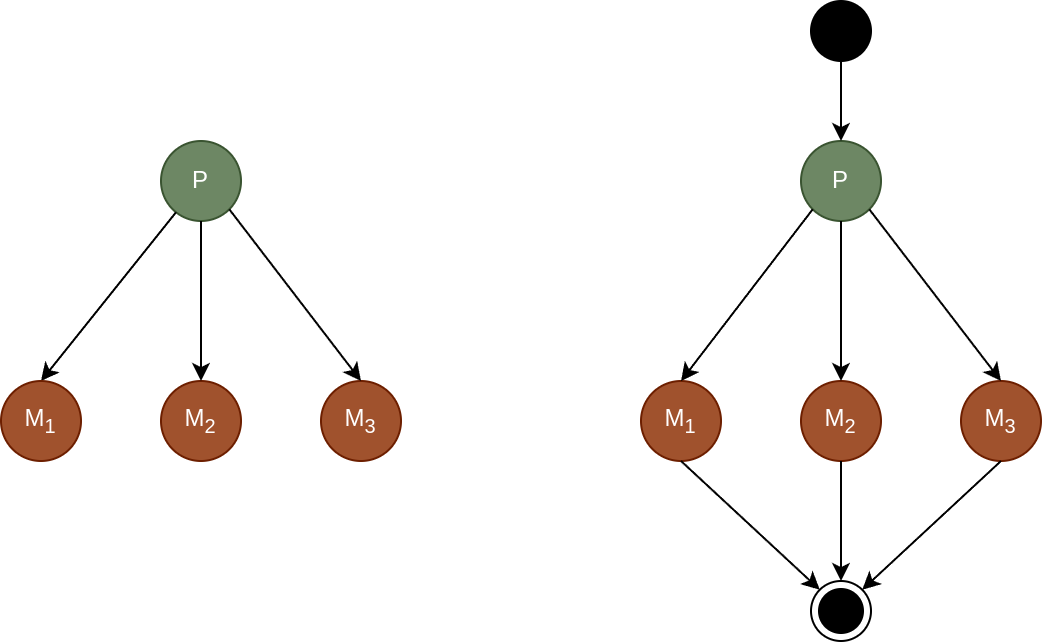
\includegraphics[scale=0.3]{../images/parallel_group.png}
	\caption{Parallel group - topology and paths}
    \label{fig:parallel_group}
\end{figure}

\subsection{Route group}

The third group type is route group. In this group, each job has a predefined route through the components of the group, and this route can differ from job to job. When a job enters this group, it is directed to the first component on its route, and then second, all the way to the last one. Figure \ref{fig:route_group} shows a route group topology on the left, and several possible paths DAGs on the right. Paths can go through all components in any order, they can contain only a subset of components, the components can be repeated in the paths, and they can even contain no components. Route group nodes are named R.

\begin{figure}[!htbp]
	\centering
	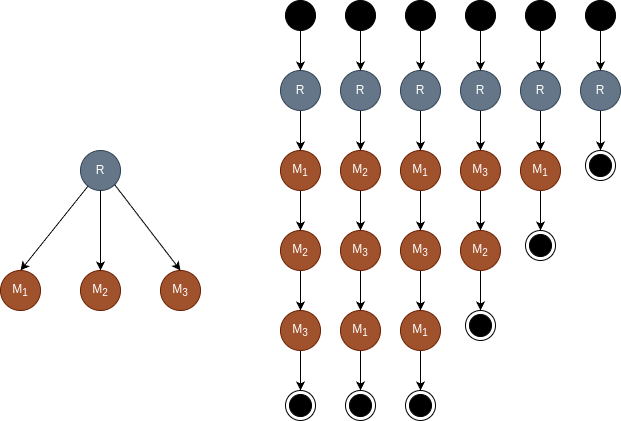
\includegraphics[scale=0.3]{../images/route_group.png}
	\caption{Route group - topology and paths}
    \label{fig:route_group}
\end{figure}

\subsection{Open group}

The fourth and the last group type is open group. In this group, each job contains a multiset of components of the group, and the job has to be processed in each component of the multiset, but it is up to the scheduler to determine the order of processing. All the same rules for paths in the route group apply here - a path can contain all components, it can contain some components, components can be repeated, and it can contain no components. Figure \ref{fig:open_group} shows an open group topology on the left, and several possible paths DAGs on the right. Open group nodes are named O. The DAG notation is expanded here to be able to represent open groups. In each path, all the components of open groups are connected to it by dashed lines. When the job arrives at an open group node, it has to go through all its components in any order, and then it proceeds to the next node in the path.

\begin{figure}[!htbp]
	\centering
	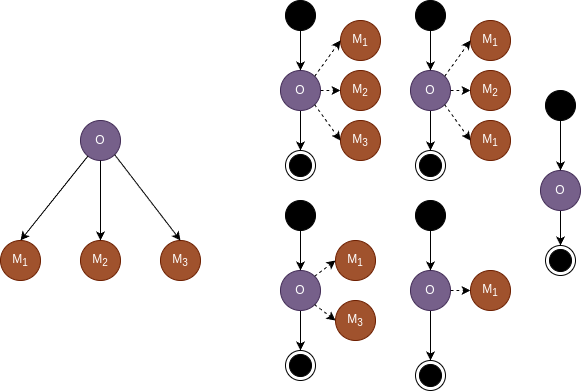
\includegraphics[scale=0.3]{../images/open_group.png}
	\caption{Open group - topology and paths}
    \label{fig:open_group}
\end{figure}

\section{Machine environments}
\label{sec:machine_environments}
The scheduling model described in \citep{pinedo2016scheduling} defines several machine environments. Here, we will go over each one of them, and describe how they can be implemented using the hierarchical topology representation. In other words, here we will describe how our topology model handles $\alpha$ entries from the scheduling problem definition.

The first environment is $1$ (single machine). This can be very easily achieved using a topology that contains a single machine element.

Several environments can be achieved using a parallel group topology element. These are $P_m$ (identical machines in parallel), $Q_m$ (machines of different speeds in parallel) and $R_m$ (unrelated machines in parallel). Machines and jobs can be divided into several types, and we can define the processing time for each combination of machine type and job type.

The machine environment $F_m$ (flow shop) can be achieved using a serial group topology element.

The machine environment $FF_c$ (flexible flow shop) consists of $c$ stages in series, where each stage contains a number of machines in parallel. Figure \ref{fig:flexible_flow_shop} shows how this environment can be achieved, with topology at the top and paths DAG at the bottom.

\begin{figure}[!htbp]
	\centering
	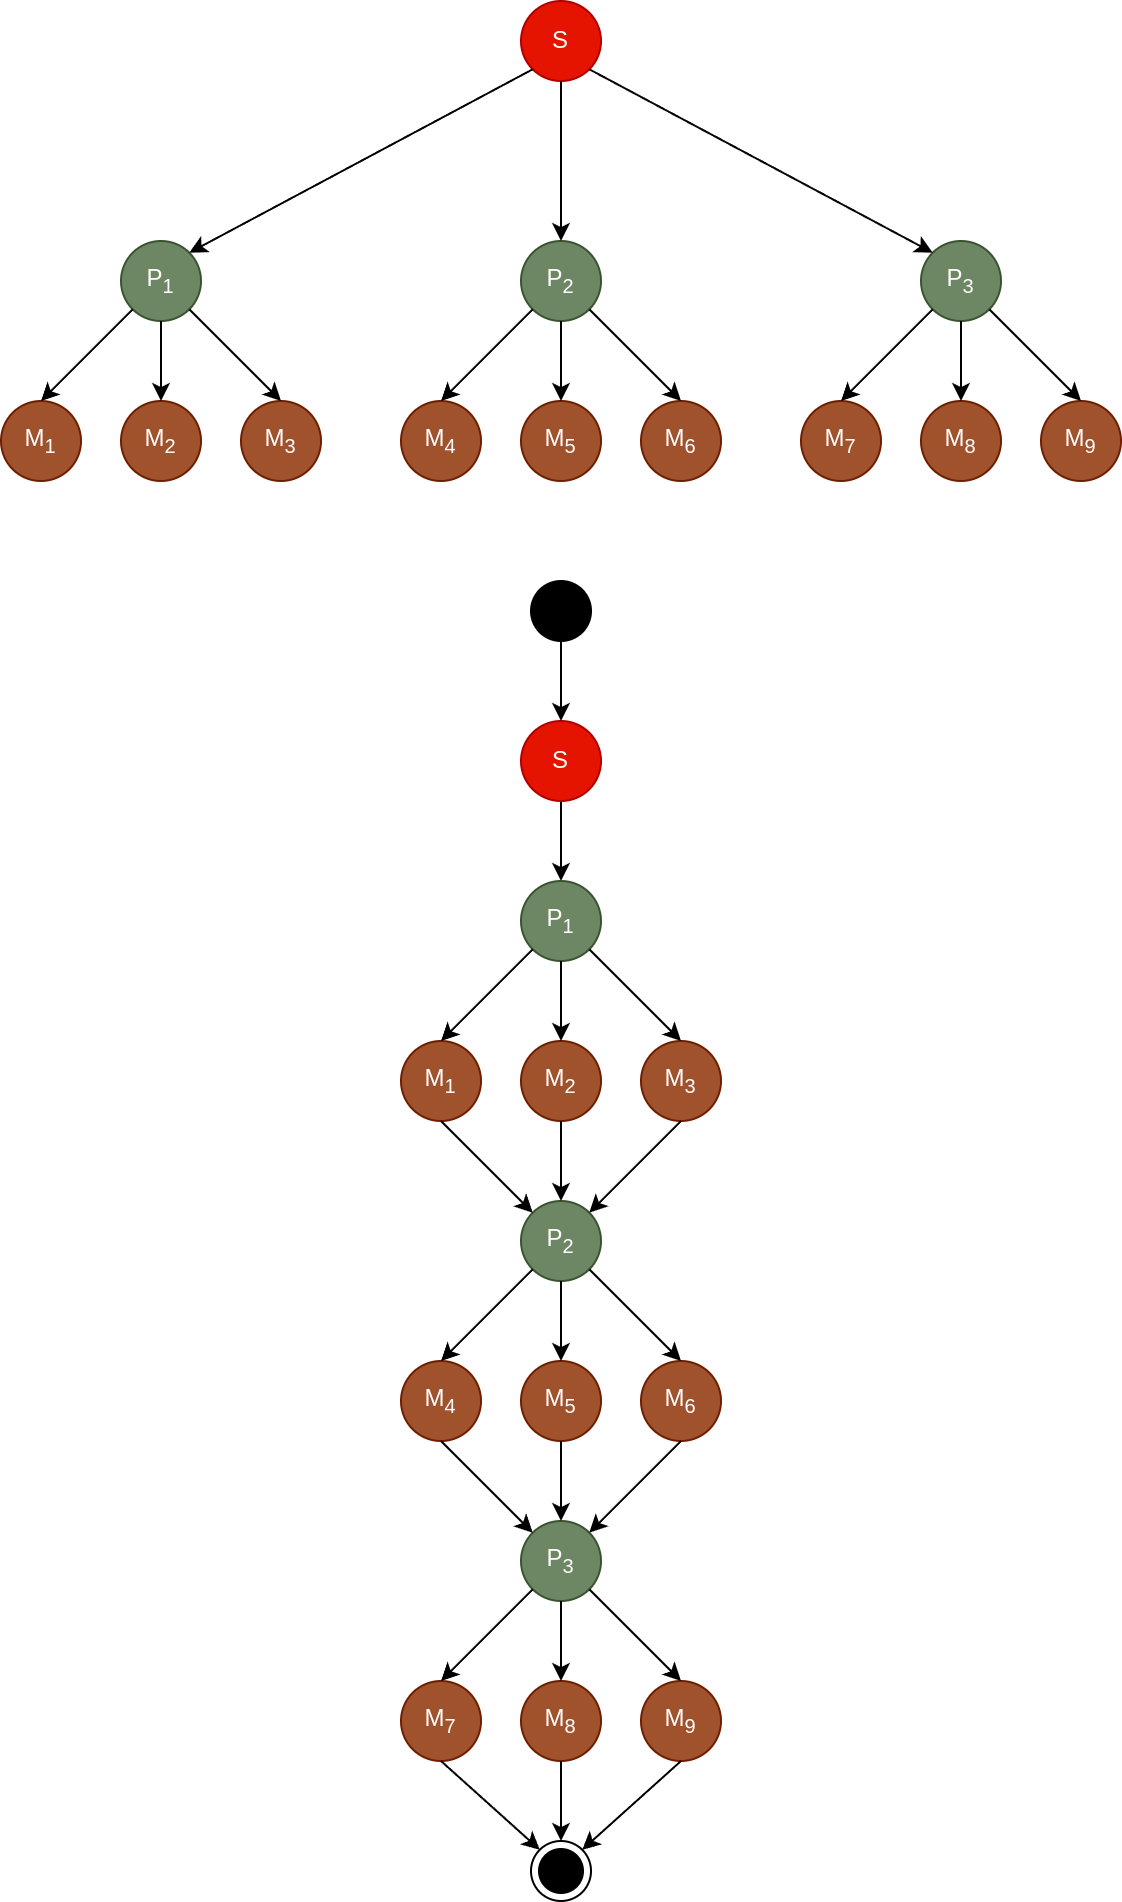
\includegraphics[scale=0.3]{../images/flexible_flow_shop.png}
	\caption{Flexible flow shop - topology and paths}
    \label{fig:flexible_flow_shop}
\end{figure}

The machine environment $J_m$ (job shop) consists of several machines, and each job has its own predetermined route through the machines of the job shop. This environment can be achieved using a route group topology element.

The machine environment $FJ_c$ (flexible job shop) consists of $c$ stages, and each stage contains several machines in parallel. Each job has its predetermined route through the system, and at every stage any machine in parallel can process the job. Figure \ref{fig:flexible_job_shop} shows one way to achieve this environment, with topology at the top and several possible paths DAGs at the bottom.

\begin{figure}[!htbp]
	\centering
	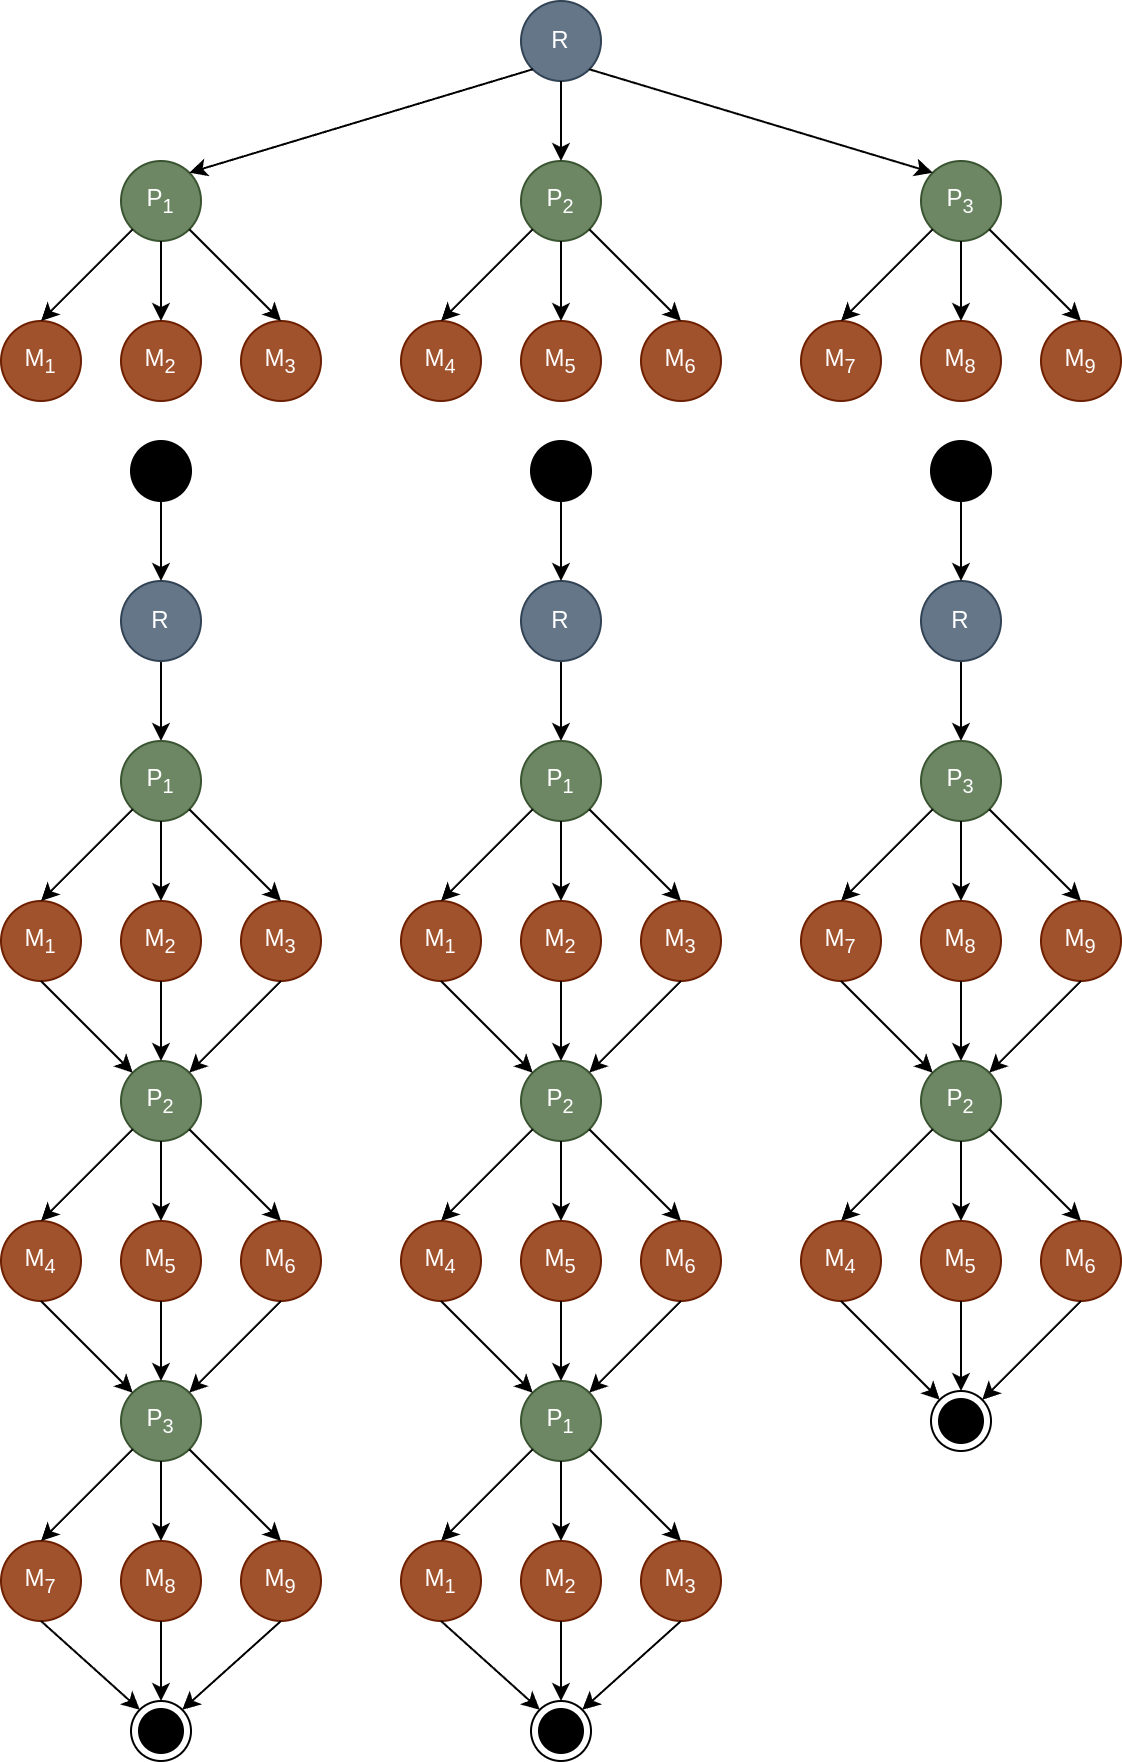
\includegraphics[scale=0.3]{../images/flexible_job_shop.png}
	\caption{Flexible job shop - topology and paths}
    \label{fig:flexible_job_shop}
\end{figure}

Finally, the machine environment $O_m$ (open machines) consists of $m$ machines, where each job has to be processed on each machine, but there are no restrictions regarding the routing of the job, and it is up to the scheduler to determine a route for each job. This environment can be achieved using an open group topology element.

As we have demonstrated, the hierarchical topology representation is a very versatile representation system. It is capable of implementing all the standard types of machine environments, but it can also implement environments which are much more complex, due to its capabilities being defined by recursive rules.
\chapter{Events model}
\label{sec:events_model}

In this chapter, we will describe the second component of the hierarchical topology representation, which is its events model.

\section{Execution model}
\label{sec:execution_model}

To simulate the execution of a sequence of jobs on a machine topology, we need to define the execution model. This model consists of several components.

The first component is machines. Machines can be divided into one or more machine types. Machines are organized in a topology, and the processing at each part of the system follows the rules set down in chapter \hyperref[sec:topology_model]{3.1}.

The second component is jobs. Jobs can be divided into one or more job types. For each job type, we can define the processing time on each machine type. We can also define the forbidden combinations of job types and machine types, and such job types can not execute on such machine types. This can affect possible paths through the topology, most prominently in parallel groups.

For each job, we can define several characteristics. The first one is release date, which is the time at which the job arrives at the system. The second one is due date, which is the time at which the job is expected to finish its execution. The third and final one is weight, which is a priority factor of the job.

Each job has its paths DAG. When a job starts its execution in the system, it starts at the source of its DAG. Whenever it finishes execution on a machine or group, it is moved to the next node in the DAG. When it reaches the sink of the DAG, the processing for it finishes.

The execution model is based on events. When the system starts, some events are created. The simulator consumes events one by one. Consumption of an event may lead to the creation of new events. The execution stops when there are no more events to consume. All event types are described in chapter \ref{sec:event_types}.

\section{Event types}
\label{sec:event_types}

There are a total of $22$ event types, and they are all listed in Table \ref{tab:event_types}. Each event type is assigned a priority index, and the lower index means higher priority. In this case, the \textit{System exit} event has the highest priority, and the \textit{Wake machine} event has the lowest.

\begin{table}[!htbp]
    \begin{center}
        \begin{tabular}{|l|l|} 
         \hline
         Event type & Priority \\ [0.5ex] 
         \hline\hline
         System exit & 1 \\ 
         \hline
         System exit forced & 2 \\
         \hline
         System entry & 3 \\
         \hline
         Machine exit & 4 \\
         \hline
         Machine exit batch & 5 \\
         \hline
         Machine exit forced & 6 \\
         \hline
         Machine exit forced batch & 7 \\
         \hline
         Machine buffer entry & 8 \\
         \hline
         Prerequisites wait start & 9 \\
         \hline
         Prerequisites wait end & 10 \\
         \hline
         Preempt & 11 \\
         \hline
         Preempt batch & 12 \\
         \hline
         Setup start & 13 \\
         \hline
         Setup end & 14 \\
         \hline
         Setup cancel & 15 \\
         \hline
         Breakdown start & 16 \\
         \hline
         Breakdown end & 17 \\
         \hline
         Machine entry & 18 \\
         \hline
         Machine entry batch & 19 \\
         \hline
         Machine buffer entry request asynchronous & 20 \\
         \hline
         Machine buffer entry request synchronous & 21 \\
         \hline
         Wake machine & 22 \\
         \hline
        \end{tabular}
        \end{center}
        \caption{Event types and their priorities}
    \label{tab:event_types}
    \end{table}

When the system starts its execution, a priority queue is initialized with certain events. At each step of the execution, the first event is popped from the queue and consumed. Consummation of an events entails changing the internal state of the simulator, and possibly the creation of new events. This loop continues until there are no more events to consume, at which point the execution is finished. 

Each event has a timestamp, and they are ordered by it from lower to higher in the event queue. Ordering events by their respective timestamps ensures temporal consistency of the simulation.

Things get interesting when two events have an identical timestamp. Logically, this means that these events are happening at the same time. This is seemingly contradictory with the execution model which consumes events one by one. To resolve this, we apply several additional rules to the ordering of events in the event queue, to ensure a logical consistency of the simulation.

The first tie breaker is the topological order of components in the topology. They are ordered in a way that every component comes after all its predecessors, where predecessors of a component are its parent in the topology tree, and the parent's predecessors. If two events share the same timestamp, they are then sorted using the topological order relative to their respective components. This ordering ensures that changes in the topology naturally propagate from its start to its end, and that, if a job is logically performing actions across multiple components at the same timestamp, it can fairly catch up to the last component where it needs to be, before scheduling decisions are made for that component. One situation where this behavior is prominent is if, after finishing processing at a machine, the job needs to go through several groups before it arrives to the next machine. Since processing in groups is instant and serves the purpose of directing the job towards its next component, a job can do a lot of actions at logically the same timestamp, and using the topological order of components as a tie breaker allows this behavior to be executed correctly.

The second tie breaker is the priority of events. If two events share the same timestamp and machine, then they are ordered by their priorities. This property, combined with the careful ordering of event types, also serves to ensure the logical consistency of the simulation.

Finally, if two events share the same timestamp, machine, and type, then it's irrelevant in which order they are executed. All the non-trivial decision making is being made in the \textit{Wake machine} event which has some interesting properties discussed later in this section, and that is the final puzzle piece to ensuring logical consistency among events with identical timestamps.

There are two types of events - auxiliary and principal. Auxiliary events are \textit{Machine buffer entry request asynchronous}, \textit{Machine buffer entry request synchronous} and \textit{Wake machine}, while the principal events are all the remaining event types. Principal events are used for advancing the job through its paths DAG, and they are crucial for the execution of a job. On the other hand, auxiliary events are useful only for the simulator. The purpose they serve is sending signals to machines, and as such, are not important for the execution of jobs.

Next, we will describe all event types, and how they utilized to simulate a certain execution aspect of jobs.

\subsection{System entry}
The \textit{System entry} event is triggered at the start of the execution of a job, and it corresponds to the source node in its paths DAG. This is one of the event types that the event queue is initialized with prior to the start of the simulation.

\subsection{System exit}
The \textit{System exit} event is triggered at the end of the execution of a job, and it corresponds to the sink node in its paths DAG.

\subsection{System exit forced}
The \textit{System exit forced} event is triggered when the execution of a job has to be forcefully terminated. The job does not reach the sink of its DAG, but still it is removed from the system.

\subsection{Machine buffer entry}
The \textit{Machine buffer entry} event happens when a job enters the buffer of a machine or a group. In terms of processing, groups are not differentiated from machines, so a job is processed on them as well, but this processing is instant and serves the function of directing the job to the next node in its paths DAG.

\subsection{Machine entry}
The \textit{Machine entry} event signifies the start of processing of a job on a machine. Whenever the machine is free and available for processing, it takes a job from its buffer and starts its processing.

\subsection{Machine exit}
The \textit{Machine exit} event signifies the end of processing of a job on a machine. At that point, the job is directed to the next node on its paths DAG by triggering a \textit{Machine buffer entry} or a \textit{System exit} event, and another job is taken for processing from the machine's buffer, if it is not empty.

\subsection{Machine exit forced}
The \textit{Machine exit forced} event is triggered when the execution of a job on a machine has to be forcefully terminated. After that, the \textit{System exit forced} event is triggered.

\subsection{Simulator feature: buffers}
Each machine has a buffer, and this buffer can have limited capacity. When a \textit{Machine exit} event is consumed, the next machine for that job is determined. If the next machine has space in its buffer, then the job is immediately moved to its buffer. Otherwise, the job is moved back to the buffer of its current machine to allow for processing of other jobs on this machine, where it stays until its next machine can accept it in its buffer. The minimal size of a buffer is one, because a job that is being processed still has a place reserved in the buffer in case it needs to be moved back to it. The \textit{Machine buffer entry} event reduces the buffer's available capacity, and the \textit{Machine exit} event increases it. In between these two events, a job takes a place in the buffer, regardless of its stage of processing on the machine. 

\subsection{Machine buffer entry request asynchronous}
The auxiliary event \textit{Machine buffer entry request asynchronous} is used for sending a signal to a machine to check whether it can accept a job in its buffer. If the machine cannot accept the job at that moment, it remembers all unfulfilled entry requests, and acknowledges them when its buffer capacity frees up.

\subsection{Machine buffer entry request synchronous}
The auxiliary event \textit{Machine buffer entry request synchronous} is triggered by the \textit{System entry} event, and is used for entering the buffer of the root machine in the topology. If this machine cannot accept jobs in its buffer, then the job is declined, and the \textit{System exit forced} event is triggered instead, because there is no space prior to the root node buffer where the job could be kept until the buffer frees up. This request is synchronous because it requires an immediate response, while the previous event was an asynchronous request, because it could be answered whenever the machine is ready to accept a job.

\subsection{Wake machine}
The auxiliary event \textit{Wake machine} is the central event type for this system. Events are severely limited in regards to the state of the simulator that they can change on their own. Most of the changes happen through this event, and this ensures logical consistency of the system. We can imagine a situation in which, at the same time, three jobs enter the system which contains a single machine, and are directed to its buffer. This means that between three \textit{Machine buffer entry} events and one \textit{Machine entry} event, something needs to happen, where the machine would choose which job it will process first. Since the events are consumed one by one, the first \textit{Machine buffer entry} event can not move the job from the machine buffer to processing, because it is not aware of other potential events which are logically happening at the same time, but due to the limitations of the computation model, will be consumed after this event. Instead what happens is that each \textit{Machine buffer entry} event triggers a \textit{Wake machine} event. This event is a signal to the machine, saying that an event has happened which may trigger a change in the machine's internal state. It has the lowest priority, because it needs to allow all other events to happen, before it has all the information it needs to make the correct decisions. In our example, this ensures that only after all the jobs enter the machine buffer at the same logical time but on different steps of the execution of the simulation, the scheduler will decide which job will be processed first, as now it has all the information it needs. The \textit{Wake machine} event is heavily utilized among all the remaining event types.

An interesting property that the \textit{Wake machine} event should posses is that its executions in an uninterrupted succession should be idempotent. By uninterrupted succession, we mean that at a given timestamp, these events are executed one by one, without any other event types in between. For such sequences, the first event is the one applying the changes to the machine's internal state, while the rest do not change its state, as there was no new information between this \textit{Wake machine} event and the last one.

\subsection{Simulator feature: prerequisites}
Each node in a job's paths DAG may have zero or more prerequisites defined. Each prerequisite is in the following format - job $x$ has to have been completed on the machine $y$ at least $z$ times, before this job can start processing on the machine. Since a job can visit a machine multiple times due to the rules set by route and open groups, it is possible to define a prerequisite that requires that a job be processed multiple times on a machine. When the job enters the machine's buffer, if its prerequisites are not all satisfied, it waits in a stand-by mode until all the prerequisites have become satisfied, at which point the job can be processed on the machine.

\subsection{Prerequisites wait start}
The \textit{Prerequisites wait start} event is triggered when a job enters a machine buffer and it has unfulfilled prerequisites on the corresponding node in its paths DAG.

\subsection{Prerequisites wait end}
Upon the consumption of the \textit{Machine exit} event, the simulator updates all unfulfilled prerequisites whose machine and job match the machine and job of the event. If the prerequisite becomes fulfilled, and if it was the last unfulfilled prerequisite blocking a job from executing on a machine, the \textit{Prerequisites wait end} event is triggered. Then, that job becomes ready for processing on that machine.

\subsection{Simulator feature: preemptions}
It is possible to define that a combination of machine type and job type supports preemptions. In that case, the scheduler is allowed to interrupt the processing of a job, and start processing a different job. The processing time that the job had is not lost, and once the job starts processing again, it continues where it left off.

\subsection{Preempt}
The \textit{Preempt} event is triggered when a job is processing on a machine on which it can be preempted, and a job of a higher priority enters the machine buffer and becomes ready for processing. In that case, the job is preempted, and it can continue its processing later.

\subsection{Simulator feature: breakdowns}
For every machine, it is possible to define breakdowns, which are periods when the machine is not available for processing, for example due to a maintenance. Information about breakdowns is known in advance and available to schedulers for use when making decisions.

\subsection{Breakdown start}
The \textit{Breakdown start} event is triggered when a breakdown for a machine starts. Just like the \textit{System entry} events, the event queue is initialized with these events prior to the start of the simulation. If the machine is processing a job when the breakdown starts, then things get interesting. If the job can be preempted, the \textit{Preempt} event is triggered. Otherwise, the \textit{Machine exit forced} event is triggered. For this reason, a \textit{Machine exit} event has a higher priority than a \textit{Preempt} event. If the job finishes processing on a machine at the exact same time when the machine starts going into a breakdown, then we want to gracefully finish processing the job first. Considerations such as this one were used to define the priorities of event types, and their relations with one another.

\subsection{Breakdown end}
The \textit{Breakdown end} event is triggered when a breakdown for a machine ends. Then the machine can start processing jobs again, so if it has available jobs in its buffer, a \textit{Machine entry} event is triggered. This is the final event type with which the event queue is initialized prior to the start of the simulation.

\subsection{Simulator feature: setups}
A setup is a time period in which the machine is not processing any job, but is necessary for context switching from the previous job to the next one. The setup rules are defined for machine types, and they are presented in the following format - when switching from a job of type $x$ to a job of type $y$, the required setup takes $z$ time to complete. If $x$ is not specified, then the setup rule is active when starting the execution of any job of type $y$, regardless of the job type of the previous job which was processed on the machine. If $y$ is not specified, then the setup rule is active whenever the previous job was of type $x$, regardless of the type of the next job. If neither $x$ nor $y$ are specified, then the setup rule is active whenever a job starts processing on the machine. These rules are specified in an ordered list, and when a job starts executing, the simulator scans through the list, trying to find a match. The first setup rule that matches the situation becomes active, while the rest are discarded. If no matching setup rule is found, then a setup is not triggered.

\subsection{Setup start}
The \textit{Setup start} event is triggered when a setup starts. It is triggered before a \textit{Machine entry} event, but after making a decision which job will be processed next on the machine.

\subsection{Setup end}
The \textit{Setup end} event is triggered when a setup ends. It is triggered by the \textit{Setup start} event, and it triggers a \textit{Machine entry} event.

\subsection{Setup cancel}
The \textit{Setup cancel} event is triggered by a \textit{Breakdown start} event, if the breakdown occurs while a setup is active. Unlike with preemptions, the time that the machine spent on a setup is not recorded, and once the breakdown ends, the setup starts from the beginning. This was a deliberate design decision, and an argument could be made both for the setup cancel and setup preempt behaviors, but the setup cancel was chosen for this system.

\subsection{Simulator feature: batch processing}
For a machine type, it is possible to define batch processing behavior. Batch processing rules are presented in the following format - on a machine of type $x$, jobs of type $y$ can be processed in batch, and the maximum number of jobs in a batch is $z$. An alternative definition would be that each job has a size $s_i$, and the sum of all jobs which are being processed in batch cannot exceed $z$. The former, simpler model, which will be used in this thesis, is a special case of the latter model in which all job sizes $s_i$ are equal to $1$. If batch processing is supported, when a job starts processing on a machine, the simulator goes to the buffer and tries to find jobs which could be processed in batch with the current job. If they are found, they are put on the machine along with the primary job for processing. The only requirement is that all the jobs which are processed at the same time have identical processing remaining times on the machine. Alternative behavior could be that the processing lasts as long as the longest remaining processing time of any job in the batch, but this could lead to undesirable effects such as the priority inversion. The situation is the same as the interaction between setups and breakdowns, an argument could be made for both behaviors, but one was chosen for this system. In all aspects, the secondary jobs in the batch mimic the primary job in the batch, because they are being processed at that time only because the primary job is being processed and the machine supports batch processing for their type.

\subsection{Machine entry batch}
The \textit{Machine entry batch} event is triggered by the \textit{Machine entry} event when the requirements for batch processing are satisfied. This event is triggered once for every secondary job in the batch, and this rule applies to all the remaining batch event types.

\subsection{Machine exit batch}
The \textit{Machine exit batch} event is triggered by the \textit{Machine exit} event when the primary job in the batch finished processing. Because jobs can be processed in a batch only if they have identical remaining processing times, when the primary job finished processing, all the other jobs in the batch should finish processing as well.

\subsection{Machine exit forced batch}
The \textit{Machine exit forced batch} event is triggered by the \textit{Machine exit forced} event when the primary job in the batch has to forcefully finish processing.

\subsection{Preempt batch}
The \textit{Preempt batch} event is triggered by the \textit{Preempt} event when the primary job in the batch is being preempted. Since preemption rules are defined for a machine type and job type combination, just as batch rules are, if the primary job in the batch can be preempted, the secondary ones can be as well.

\section{Interactions between events}

Figure \ref{fig:interactions_between_events} shows all event types, and their interactions. Black dots are sources, and the black dots with a red border are sinks. Full arrows imply that an event always triggers another event. Dashed arrows imply that an event may or may not trigger another event. White rhombuses imply branching, which means that an event always triggers one and exactly one of the events that the rhombus is connected to. This diagram was not created with any modelling standards such as the UML in mind, but instead, the ad hoc notations described in this paragraph were used. 

Looking at the diagram, it is apparent that the \textit{Wake machine} event is at the center of the whole system, and that the effects that the other event types can have without it are only local, like a \textit{Machine entry} event triggering a \textit{Machine exit} event. For example, even the \textit{Machine entry batch} events are not triggered directly by the \textit{Machine entry} event as was described in chapter \ref{sec:event_types}, but instead, this interaction happens through the \textit{Wake machine} event. Otherwise, the system could very easily become unmantainable, with unpredictable interactions. It is easier and more reliable to guarantee logical consistency if all the non-trivial decision making is concentrated in one place, rather than dispersed across the system.

\begin{figure}[!htbp]
	\centering
	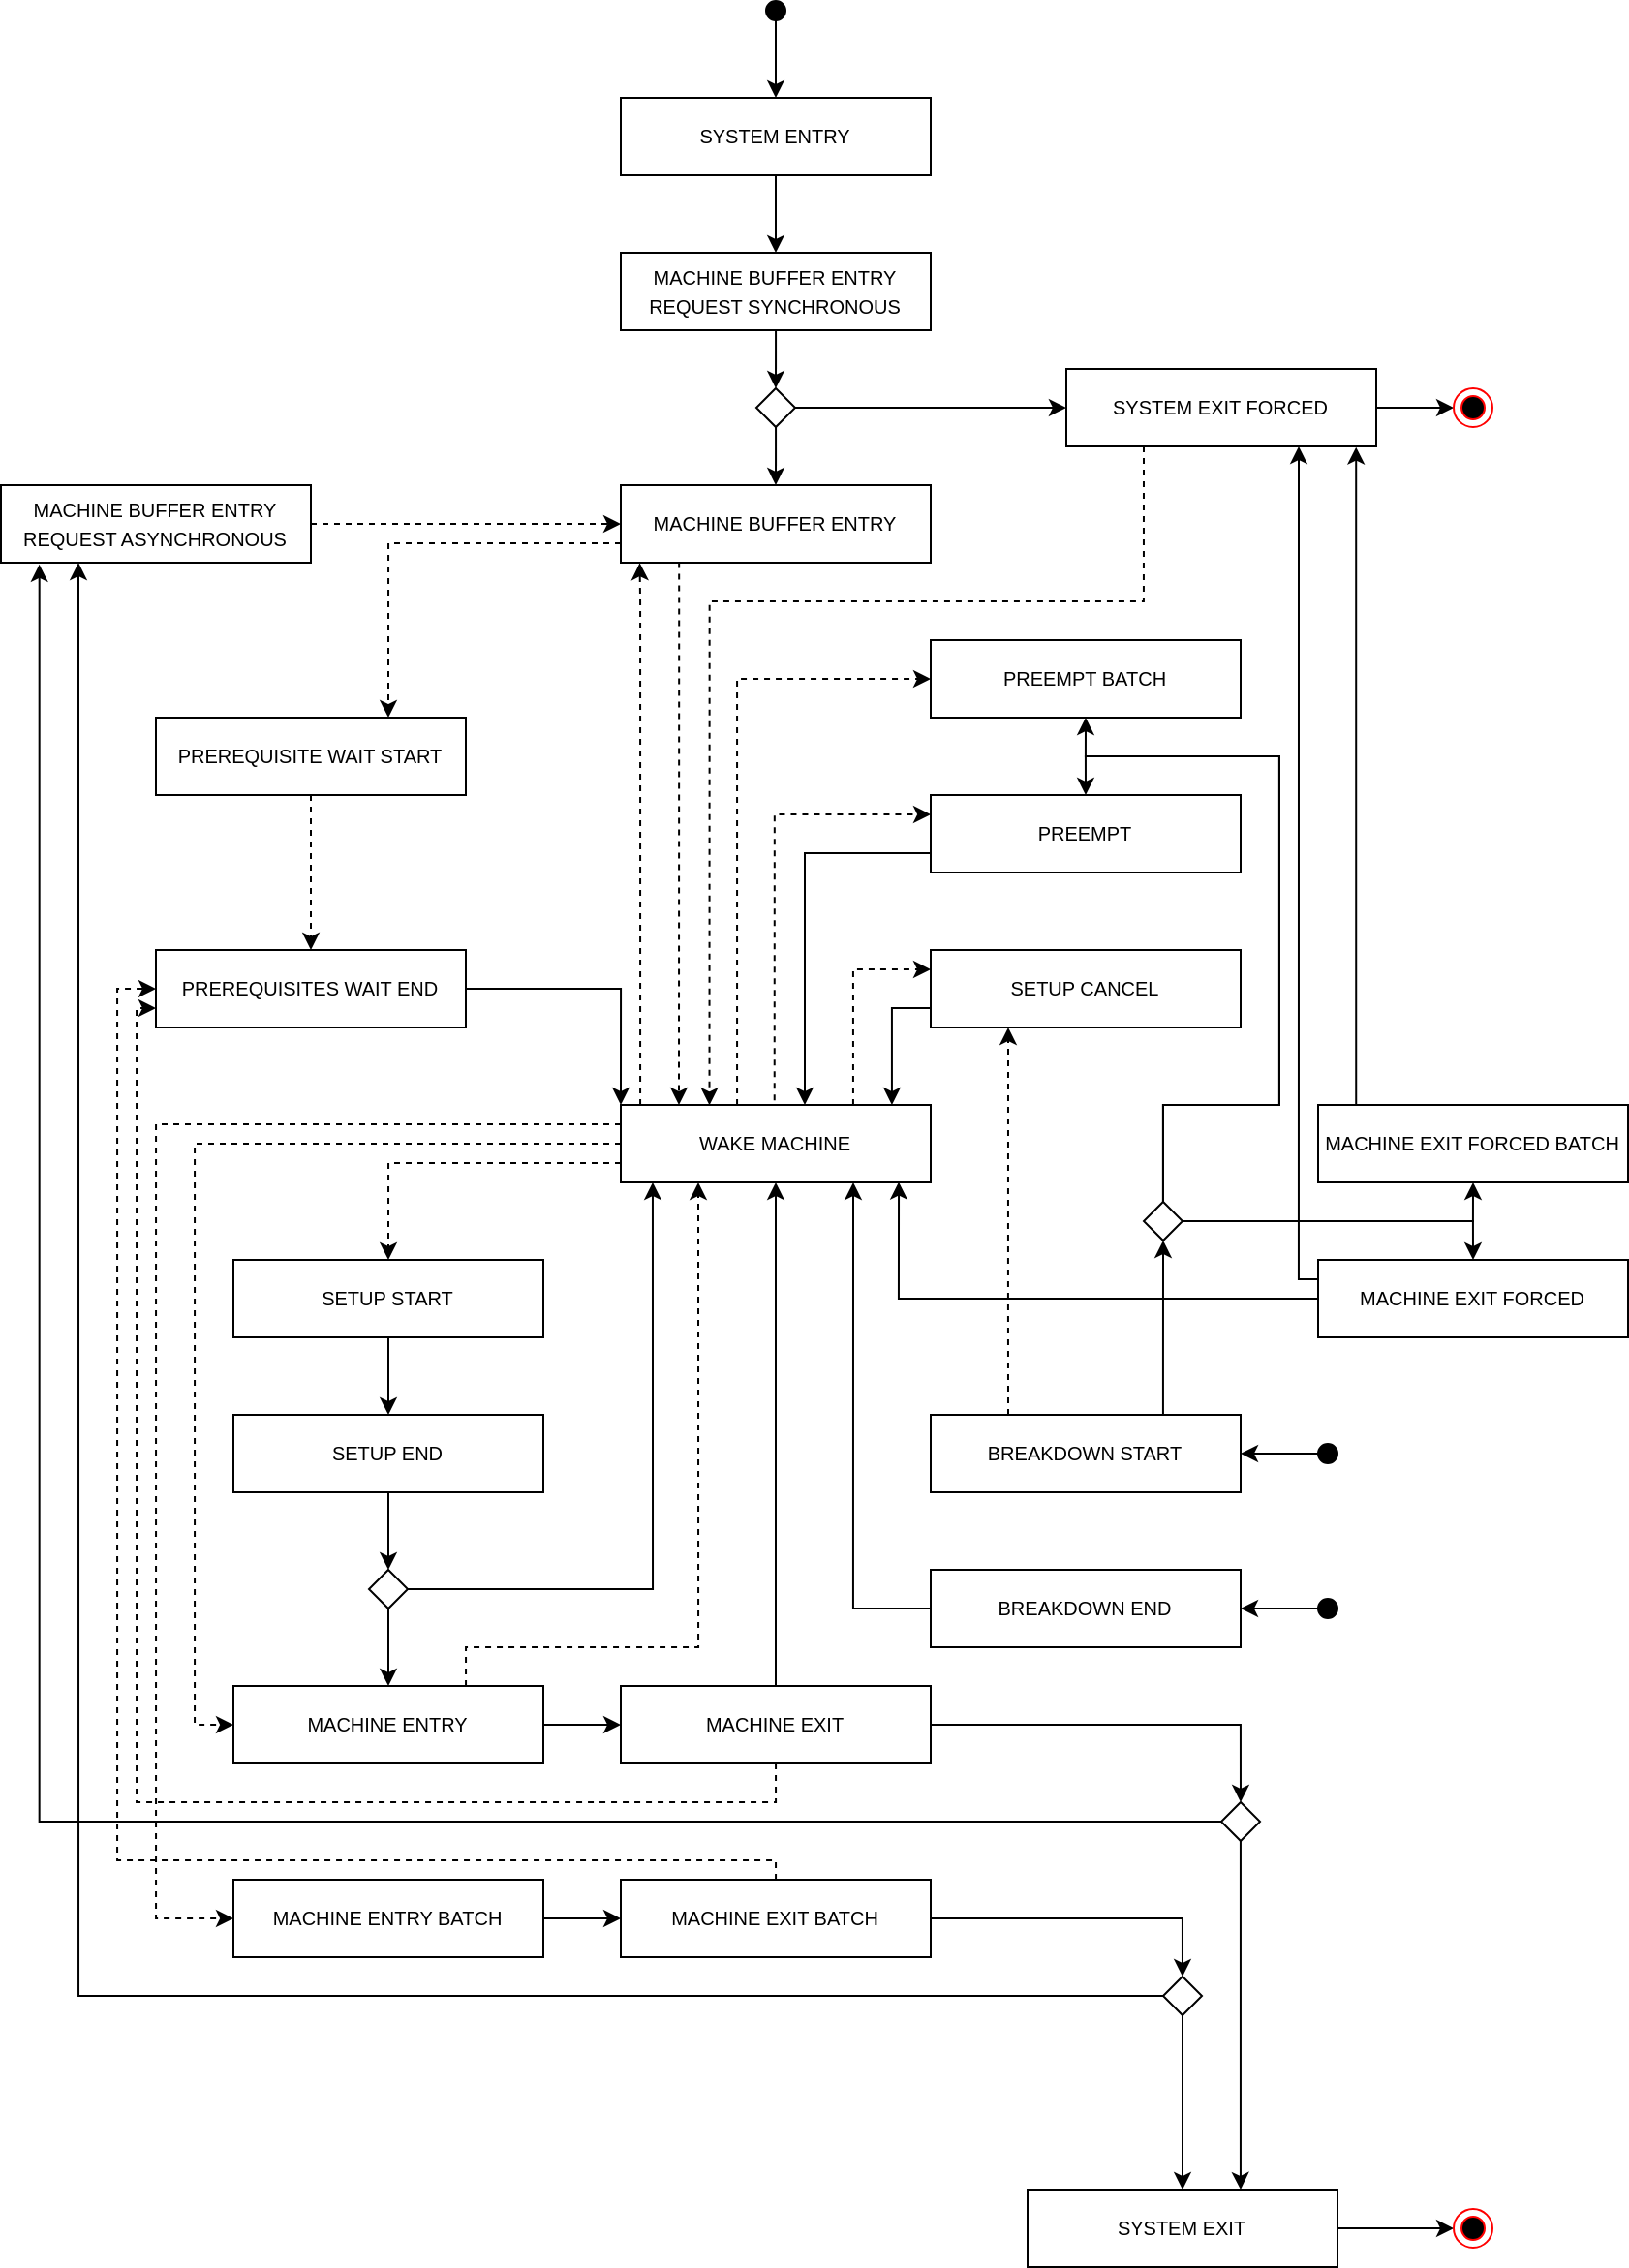
\includegraphics[scale=0.24]{../images/events.png}
	\caption{Interactions between events}
    \label{fig:interactions_between_events}
\end{figure}

\section{Execution examples}
\label{sec:execution_examples}

To demonstrate how events can be utilized to simulate the execution of a job in a topology, we will go through a couple of examples. In these examples, the auxiliary event types (\textit{Machine buffer entry request asynchronous}, \textit{Machine buffer entry request synchronous} and \textit{Wake machine}) will be excluded for simplicity, as they are not important for a job and its execution steps.

\subsection{Single machine}

Execution on the environment $1$ (single machine) can be simulated using the following sequence of events, where the machine has an identifier 1:
\begin{itemize}
    \item System entry
    \item Machine 1 buffer entry
    \item Machine 1 entry
    \item Machine 1 exit
    \item System exit
  \end{itemize}

\subsection{Flow shop}

Execution on the environment $F_3$ (flow shop with three machines, equivalent to a serial group) can be simulated using the following sequence of events, where a serial group has an identifier 1, and the machines have identifiers 2-4:
\begin{itemize}
    \item System entry
    \item Machine 1 buffer entry
    \item Machine 1 entry
    \item Machine 1 exit
    \item Machine 2 buffer entry
    \item Machine 2 entry
    \item Machine 2 exit
    \item Machine 3 buffer entry
    \item Machine 3 entry
    \item Machine 3 exit
    \item Machine 4 buffer entry
    \item Machine 4 entry
    \item Machine 4 exit
    \item System exit
  \end{itemize}

\subsection{Parallel machines}

Execution on the environment $P_3$ (three machines in parallel) can be simulated using the following sequence of events, where a parallel group has an identifier 1, and the machines have identifiers 2-4:
\begin{itemize}
    \item System entry
    \item Machine 1 buffer entry
    \item Machine 1 entry
    \item Machine 1 exit
    \item Machine 3 buffer entry
    \item Machine 3 entry
    \item Machine 3 exit
    \item System exit
  \end{itemize}

\section{Processing characteristics and constraints}
\label{sec:processing_characteristics_and_constraints}

The scheduling model described in \citep{pinedo2016scheduling} defines a number of processing characteristics and constraints. Here, we will go over each one of them, and describe how they can be achieved using our events model. In other words, here we will describe how our events model handles $\beta$ entries from the scheduling problem definition.

Release date ($r_j$) is the time at which the job $j$ enters the system and becomes ready for processing. This can be easily specified for every job, along with the due date ($d_j$) and weight ($w_j$) of the job.

Preemptions ($prmp$) are achieved using the \textit{Preempt} and \textit{Preempt batch} events.

Precedence constraints ($prec$) allow requiring that one or more jobs have to be completed before another job can start processing. They are achieved using the \textit{Prerequisites wait start} and \textit{Prerequisites wait end} events.

Sequence dependent setup times ($s_{jk}$) are what we have called setups earlier in this chapter, and they are achieved using the \textit{Setup start}, \textit{Setup end} and \textit{Setup cancel} events.

Job families ($fmls$) are equivalent to the job types mechanism. In this context, job families dictate the setup time between jobs, and this can be easily specified because our setup rules work with job types.

Batch processing ($batch(b)$) is achieved using the \textit{Machine entry batch}, \textit{Machine exit batch}, \textit{Machine exit forced batch} and \textit{Preempt batch} events.

Breakdowns ($brkdwn$) are achieved using the \textit{Breakdown start} and \textit{Breakdown end} events.

Machine eligibility restrictions ($M_j$) allow specifying which jobs cannot be processed on which machines. They are achieved by specifying the forbidden machine types for each job type.

Permutation ($prmu$) is a constraint in flow shop environments which requires that queues in front of each other operate according to the \textit{First In First Out (FIFO)} principle. This behavior is default in the serial group element.

Blocking ($block$) specifies that if a flow shop has buffers of a limited size between subsequent machines, when the upstream buffer is full, a machine is not allowed to release a job whose processing it has finished. This behavior is implemented in machine buffers with limited size.

No-wait ($nwt$) is a phenomenon which may occur in flow shops, where jobs are not allowed to wait between two successive machines. In other words, their processing in the flow shop needs to be uninterrupted between machines. This behavior can be achieved by specifying that a serial group and all its components share the same buffer whose size is equal to one. In that case, only when a job leaves the serial group will the buffer free up and the serial group will be ready to accept another job.

Recirculation ($rcrc$) allows jobs to be processed on the same components multiple times. This behavior is allowed in route and open groups.

As we have demonstrated, the events model presented in this chapter is a versatile model which fully covers the processing characteristics and constraints of the machines and jobs scheduling model.
\chapter{Evaluation model}
\label{sec:evaluation_model}

In this chapter, we will describe the third and the final component of the hierarchical topology representation, which is its evaluation model.

\section{Evaluation data}
\label{sec:evaluation_data}
When the simulation is running, the simulator will occasionally update the data about jobs. The characteristics which are available to the objective function are the job's release time, due time and weight. When the processing for a job finished, the simulator will also update the exit time for a job. These four parameters are used in most of the objective functions.

Another useful parameter which was not specified in the scheduling model, but which is natural for this representation is the job status upon simulation end. If the job reaches a sink node in its DAG, then it finishes processing normally, and the request was fulfilled. If the job does not reach a sink node in its DAG, but it still leaves the system, that means that a \textit{System exit forced} event was triggered, and that the request was not fulfilled. 

The third option is that a job does not finish its processing, and instead remains stuck in come component's buffer. This can happen if the job is waiting for a prerequisite that cannot be fulfilled. In that case, all events will be consumed, and there will nothing left to change the job's state.

To summarize, the five parameters for an objective function are the job's release time, due time, exit time, weight and status, which can be successfully terminated, unsuccessfully terminated and unterminated. All the objective functions use a combination of these parameters to produce a result for a job, and an aggregation of results for all jobs is used to produce the final score for the schedule.

\section{Objective functions}
\label{sec:objective_functions}

The scheduling model described in \citep{pinedo2016scheduling} describes several objective functions. In this chapter, we will list several of these functions for the sake of completeness, and to show some common objective functions in scheduling problems. In other words, here we will describe how our evaluation model handles the $ \gamma $ entries from the scheduling problem definition.

In this chapter and throughout this thesis, we will use the following notations for objective functions - for a job $j$, we will use $r_j$ to denote its release time, $d_j$ to denote its due time, $e_j$ to denote its exit time, $w_j$ to denote its weight, and $s_j$ to denote its status.

Lateness of a job is defined as $L_j = e_j - d_j$. Since lateness can be negative, another metric is introduced, which is tardiness, defined as $T_j = max(L_j, 0)$. The unit penalty of a job is defined as $U_j = e_j > d_j$, and it can be zero or one. Earliness of a job is defined as $E_j = max(d_j - e_j, 0)$.

The table \ref{tab:objective_functions_table} shows some objective functions, along with their formulas. All of these functions can be implemented using the data presented in chapter \ref{sec:evaluation_data}. This means that the evaluation model of the hierarchical topology representation fully covers the evaluation of the machines and jobs scheduling model.

\begin{table}[!htbp]
    \begin{center}
        \begin{tabular}{|l|l|} 
         \hline
         Objective function & Formula \\ [0.5ex] 
         \hline\hline
         Makespan & $ max(e_1, e_2, ..., e_n) $ \\ 
         \hline
         Maximum lateness & $  max(L_1, L_2, ..., L_n) $ \\ 
         \hline
         Total weighed completion time & $ \sum_{j} w_j e_j $ \\ 
         \hline
         Discounted total weighted completion time, $ 0 < r < 1$ & $ \sum_{j} w_j (1 - e^{-r e_j}) $ \\ 
         \hline
         Total weighted tardiness & $ \sum_{j} w_j T_j $ \\ 
         \hline
         Weighted number of tardy jobs & $ \sum_{j} w_j U_j $ \\ 
         \hline
         Total earliness plus total tardiness & $ \sum_{j} E_j + \sum_{j} T_j $ \\ 
         \hline
        \end{tabular}
        \end{center}
        \caption{Examples of objective functions}
    \label{tab:objective_functions_table}
    \end{table}

In chapter \ref{sec:scheduling}, we have defined scheduling problems using the triplet $\alpha | \beta | \gamma$. Over the past three chapters, we have introduced the hierarchical topology representation, and we have shown that this representation can express any scheduling problem which can be expressed by this triplet. This proves that it is a versatile and expressive representation system. The question that is left to answer is how this representation can be used to solve scheduling problems, and this question will be answered in the following chapters.
\chapter{Optimization model}
\label{sec:optimization_model}

In this chapter, we will describe the framework which can be used to build modular optimization algorithms. While these concepts can be used for a broad range of problems, we will use them for scheduling in the following chapters. 

\section{Components of optimization algorithms}
\label{sec:components_of_optimization_algorithms}

In this chapter, we will describe the components which can be used to build optimization algorithms. It is important to note that the goal of optimization is to solve problems. The premise that we are working with is that we want to solve a problem, and we are defining tools that we can use to solve it.

\subsection{Genotype}
\label{sec:genotype}

The first component is the genotype for the problem. Genotype is a technical term for problem representation, and it entails data structures which store some information about the problem solution. If we define a genotype, then we are able to encode and represent solutions to the problem we are solving.

It is important to note that the word genotype has a somewhat different connotation throughout literature from what we will use it here for. In literature, terms genotype and phenotype are defined and distinguished. Genotype refers to data structures which can be manipulated and which store information about a problem solution. Genotype can be mapped to an actual problem solution, which is called phenotype. Some representations have a clear distinction between genotype and phenotype, while in others they are the same.

In the context of this thesis, the word genotype will be used as an umbrella term genotype, phenotype, and the optional mapping process from the former to the latter. This is because we will define operators which manipulate the genotype and that will be most interesting to us, while the phenotype mapping process will be implicit. The reasoning behind this decision is that the relation between genotype and phenotype depends only on the representation system, and we want to work on an abstract level, with operators that transform the data structures which contain an encoding for the problem solution.

To recap, if we define a genotype for a problem, then we are able to represent and describe its solutions.

\subsection{Evaluation function}
\label{sec:evaluation_function}

The next component is the evaluation function. This is a function which maps a genotype to a number. It is used to measure the quality of solutions. Since we will be solving minimization problems in this thesis, evaluation functions will be used to measure how bad of a solution a particular genotype is, and the goal will be to minimize this measure.

If we can define an evaluation function for a problem, then we can compare two solutions and determine which one is better. In our case, the better solution will be the one with the lower evaluation function value.

\subsection{Creation operator}
\label{sec:creation_operator}

The next component is the creation operator. This is an operator which creates a random genotype. It doesn't take any arguments, but it does require some metadata about the problem and its domain. For example, if we are solving a numerical optimization problem, then this metadata consists of the number of variables and the domain of each one. It can also have some parameters, it terms of numerical optimization this can be the distribution from which the points are sampled, but it is important that, once the operator is initialized and put in use, it shouldn't require any arguments to create a genotype.

The creation operator should contain an element of randomness, as we want to construct different genotypes each time we apply it. The result can be completely random, or it can be constructed using a randomized heuristic. An example of an algorithm which uses heuristics to construct solutions is the GRASP algorithm \citep{grasp}.

With the components we have defined, we are able to encode problem solutions, we can evaluate them, and we can randomly construct them. This is enough to create our first optimization algorithm, random search. One application of random search can be found in \citep{random_search}. The pseudocode for random search can be found in algorithm \ref{alg:random_search}.

\begin{algorithm}[!htbp]
    \caption{Random search}
    \label{alg:random_search}
    \KwIn{$evaluation\_function$, $creation\_operator$, $number\_of\_iterations$}
    \KwOut{$(best\_solution, best\_score)$}

    $x \gets NULL$\;
    $s \gets \infty$\;
    \For{$iter \gets 1$ \KwTo $number\_of\_iterations$}{
        $x' \gets creation\_operator.create()$\;
        $s' \gets evaluation\_function.evaluate(x')$\;
        \If{$s' < s$}{
            $(x, s) \gets (x', s')$\;
        }
    }
    \Return $(x, s)$\;
    \end{algorithm}
    
\subsection{Neighborhood operator}
\label{sec:neighbood_operator}

The next component is the neighborhood operator. This is an operator which takes as an argument a genotype, and returns a list of genotypes. These genotypes are considered neighbors of the original genotype, which means that they are close in the search space. Neighbors are constructed by applying changes to the argument genotype. The severity of these changes can impact the size of the resulting neighborhood.

An algorithm which uses a neighborhood operator is the hill-climbing search \citep{artificial_intelligence}, whose pseudocode can be found in algorithm \ref{alg:hill_climbing_search}. This simple, greedy algorithm is often used as a local heuristic in other search algorithms.

\begin{algorithm}[!htbp]
    \caption{Hill-climbing search}
    \label{alg:hill_climbing_search}
    \KwIn{$evaluation\_function$, $creation\_operator$, $neighborhood\_operator$, $number\_of\_iterations$}
    \KwOut{$(best\_solution, best\_score)$}

    $x \gets creation\_operator.create()$\;
    $s \gets evaluation\_function.evaluate(x)$\;

    \For{$iter \gets 1$ \KwTo $number\_of\_iterations$}{
        $x' \gets x$\;
        $neighborhood \gets neighborhood\_operator.generate(x')$\;
        \For{$x'' \in neighborhood$}{
            $s'' \gets evaluation\_function.evaluate(x'')$\;
            \If{$s'' < s$}{
                $(x, s) \gets (x'', s'')$\;
            }
        }

        \If{$x' = x$}{
            $break$\;
        }
    }

    \Return $(x, s)$\;
    \end{algorithm}

An advantage of separating the genotype definition from the genotype operators definition is that this framework allows building multiple operators of the same type for one genotype definition. An algorithm which utilizes multiple neighborhood operator definitions is the variable neighborhood search \citep{variable_neighborhood_search}, whose pseudocode can be found in algorithm \ref{alg:variable_neighborhood_search}. The \textit{local search algorithm} parameter can be any search heuristic, and a good candidate is the hill-climbing search.

\begin{algorithm}[!htbp]
    \caption{Variable neighborhood search}
    \label{alg:variable_neighborhood_search}
    \KwIn{$evaluation\_function$, $creation\_operator$, $neighborhood\_operators$, $local\_search\_algorithm$,  $number\_of\_iterations$}
    \KwOut{$(best\_solution, best\_score)$}

    $x \gets creation\_operator.create()$\;
    $s \gets evaluation\_function.evaluate(x)$\;

    \For{$iter \gets 1$ \KwTo $number\_of\_iterations$} {

        $k \gets 0$\;
        \While{$k < neighborhood\_operators.size()$}{
            
            $x' \gets neighborhood\_operators[k].generate(x).randomElement()$\;
            $(x'', s'')$ $\gets$ $local\_search\_algorithm.search($ $evaluation\_function,$ \newline \hspace*{1em} $ neighborhood\_operator, x')$\;
        
            \If{$s'' < x$}{
                $(x, s) \gets (x'', s'')$\;
                $k \gets 0$\;
            }  
            \Else{
                $k \gets k + 1$\;
            }
        }      
    }

    \Return $(x, s)$\;
    \end{algorithm}

\subsection{Perturbation operator}
\label{sec:perturbation_operator}

The next component is the perturbation operator. This operator takes a genotype as an argument, and returns one genotype as a result. It can be considered as a special case of a neighborhood operator where the length of the resulting neighborhood is always equal to one, these operators are distinguished for two reasons. The first reason is that the neighborhood operators are usually used in iterative search algorithms, while the perturbation operators are used in evolutionary algorithms, where the operator is more frequently called a mutation operator. The second reason is that the neighborhood operators are expected to apply less severe changes to the argument genotype than the perturbation operators. 

The idea behind a perturbation operator is that takes a genotype and changes it more or less severely. These operators can be used to effectively escape local optima.

One algorithm which uses a perturbation operator is the iterated local search \citep{iterated_local_search}, whose pseudocode can be found in algorithm \ref{alg:iterated_local_search}. 

\begin{algorithm}[!htbp]
    \caption{Iterated local search}
    \label{alg:iterated_local_search}
    \KwIn{$evaluation\_function$, $creation\_operator$, $neighborhood\_operator$, $perturbation\_operator$, $local\_search\_algorithm$,  $number\_of\_iterations$}
    \KwOut{$(best\_solution, best\_score)$}

    $x \gets creation\_operator.create()$\;
    $s \gets evaluation\_function.evaluate(x)$\;

    \For{$iter \gets 1$ \KwTo $number\_of\_iterations$} {
        $x' \gets perturbation\_operator.perturbate(x)$\;
        $(x'', s'')$ $\gets$ $local\_search\_algorithm.search($$evaluation\_function,$ \newline \hspace*{1em} $ neighborhood\_operator, x')$\;
        \If{$s'' < s$}{
            $(x, s) \gets (x'', s'')$\;
        }
    }

    \Return $(x, s)$\;
    \end{algorithm}

\subsection{Combination operator}
\label{sec:combinatino_operator}

The final component is the combination operator. This operator takes two genotypes as arguments, and produces one genotype as a result. In evolutionary algorithms, these operators are more commonly called crossover operators. The idea behind them is that, if two genotypes have good genetic material, combining them has the potential to produce an even better genotype. We will see several examples of algorithms which utilize combination operators in chapter \ref{sec:optimization_algorithms}.

\section{Optimization algorithms}
\label{sec:optimization_algorithms}

In this chapter, we will use the tools which we have defined to describe several optimization algorithms. It is here that we will see the biggest advantage of building optimization algorithms in a modular way. 

To reiterate, the workflow of solving a problem is - define the problem, define the genotype for the problem, define the evaluation function and lastly, define the operators for the genotype. All of these become reusable components from one optimization algorithm to another. The only differences between these algorithms are which operators they require, how they choose solutions from the population, which operators they apply on them, and how they update the population at the end of each iteration. Not only are the problem-specific components reusable from one optimization algorithm to another, but the algorithms themselves can be used interchangeably on the same problem.

For iterative algorithms, it is possible to define several stopping criteria. For this purpose, we will use the number of evaluations of the evaluation function, because this is the most expensive operations for the problems we will solve, and the overhead that the algorithm itself introduces is negligible compared to simulating and evaluating scheduling systems.

\subsection{Steady-state genetic algorithm}
\label{sec:ssga}

The steady-state genetic algorithm (SSGA) \citep{ssga} is an algorithm which requires creation, combination and perturbation operators. At the start of the algorithm, the population is initialized using the creation operator. Every iteration consists of the following steps: uniformly choose two random parents, apply the combination operator on them to create their child, use the perturbation operator on the newly created child, evaluate the child, insert the child into the population, and remove the worst individual from the population to keep its size constant. The population is sorted by the individuals' score, and the final result is the best individual when the algorithm terminates.

The size of the population is the only hyperparameter of the algorithm. The pseudocode for the algorithm can be found in algorithm \ref{alg:ssga}. The $initializePopulation$ function returns a sorted population of randomly created individuals. The $insertSorted$ function inserts an individual and its fitness into the population, and the $trim$ function removes excess individuals from the population to keep its size constant. These functions will be used throughout all of the metaheuristics.

\begin{algorithm}[!htbp]
    \caption{Steady-state genetic algorithm}
    \label{alg:ssga}
    \KwIn{$evaluation\_function$, $creation\_operator$, $combination\_operator$, $perturbation\_operator$, $population\_size$,  $number\_of\_iterations$}
    \KwOut{$(best\_solution, best\_score)$}

    $population = initializePopulation(creation\_operator, population\_size)$\;

    \For{$iter \gets 1$ \KwTo $number\_of\_iterations$} {
        $p_1 \gets population.randomElement()$\;
        $p_2 \gets population.randomElement()$\;
        $x \gets combination\_operator.combine(p_1, p_2)$\;
        $x' \gets perturbation\_operator.perturbate(x)$\;
        $s' \gets evaluation\_function.evaluate(x')$\;
        $population.insertSorted((x', s'))$\;
        $population.trim(population\_size)$\;
    }

    \Return $population.bestElement()$\;
    \end{algorithm}

\subsection{Generational genetic algorithm}
\label{sec:gga}

The generational genetic algorithm (GGA) \citep{gga} is an algorithm which uses the same operators and population initialization technique as SSGA. But while SSGA changes one element of the population per iteration, GGA changes the entire population. For selection, we will use the fitness-proportional selection, also known as the roulette-wheel selection. The idea is that individuals with higher fitness have a higher chance of being chosen as parents, and this mechanism creates a selection pressure and improves the algorithm's convergence.

In roulette-wheel selection, each individual is assigned a coefficient relative to its fitness. The best individual has the coefficient $1$, while the coefficient for the worst individual is adjustable. For example, if this coefficient is $0.1$, that means that the best individual is $10$ times more likely to be chosen as a parent than the worst one. Coefficients for the remaining individuals are calculated using linear interpolation between the best and the worst individuals. A random number generator is used to sample a random number between zero and the sum of all coefficients, and binary search is used to find the individual that the sampled number corresponds to.

Another important feature is elitism, which ensures that the algorithm never loses its best found solution. While SSGA has elitism by design, in GGA it is ensured by copying the best individual to the new population in each iteration.

The hyperparameters of the algorithm are the population size and worst individual coefficient for the roulette-wheel selection. The pseudocode for the algorithm can be found in algorithm \ref{alg:gga}.

\begin{algorithm}[!htbp]
    \caption{Generation genetic algorithm}
    \label{alg:gga}
    \KwIn{$evaluation\_function$, $creation\_operator$, $combination\_operator$, $perturbation\_operator$, $population\_size$,  $worst\_individual\_coef$, $number\_of\_iterations$}
    \KwOut{$(best\_solution, best\_score)$}

    $population = initializePopulation(creation\_operator, population\_size)$\;

    \For{$iter \gets 1$ \KwTo $number\_of\_iterations$} {
        $new\_population \gets emptyList()$\;
        $roulette\_wheel \gets createRouletteWheel(population)$\;

        $new\_population.insert(population.at(0))$\;

        \For{$i \gets 2$ \KwTo $population\_size$}{
            $p_1 \gets roulette\_wheel.sampleElement()$\;
            $p_2 \gets roulette\_wheel.sampleElement()$\;
            $x \gets combination\_operator.combine(p_1, p_2)$\;
            $x' \gets perturbation\_operator.perturbate(x)$\;
            $s' \gets evaluation\_function.evaluate(x')$\;
            $new\_population.insert((x', s'))$\;
        }

        $new\_population.sort()$\;
        $population \gets new\_population$\;
    }

    \Return $population.bestElement()$\;
    \end{algorithm}

\subsection{Evolution strategy}
\label{sec:es}
Evolutionary strategies (EA) are a family of optimization algorithms closely related to genetic algorithms. An EA which we will use is similar to SSGA, and the difference is that it will create several new individuals per iteration, instead of one. In the context of EAs, this schema is known as the $(\mu + \lambda)$ schema, where the population size is $\mu$, the number of newly created individuals per iteration is $\lambda$, and the new population is selected from the combined pool of parents and newly created offspring. An alternative schema is $(\mu, \lambda)$, where the new population is selected only from offspring, and an EA which uses this schema is similar to GGA.

Hyperparameters for the algorithm are population size and the percentage which indicates the proportion of new individuals generated in each iteration, relative to the population size. The pseudocode for the algorithm can be found in algorithm \ref{alg:ea}.

\begin{algorithm}[!htbp]
    \caption{Evolution strategy}
    \label{alg:ea}
    \KwIn{$evaluation\_function$, $creation\_operator$, $combination\_operator$, $perturbation\_operator$, $population\_size$, $new\_individuals\_per\_iteration\_percentage$, $number\_of\_iterations$}
    \KwOut{$(best\_solution, best\_score)$}

    $population = initializePopulation(creation\_operator, population\_size)$\;
    $\lambda = population\_size \times new\_individuals\_per\_iteration\_percentage$\;

    \For{$iter \gets 1$ \KwTo $number\_of\_iterations$} {
        \For{$i \gets 1$ \KwTo $\lambda$}{
            $p_1 \gets population.randomElement()$\;
            $p_2 \gets population.randomElement()$\;
            $x \gets combination\_operator.combine(p_1, p_2)$\;
            $x' \gets perturbation\_operator.perturbate(x)$\;
            $s' \gets evaluation\_function.evaluate(x')$\;
            $population.insertSorted((x', s'))$\;
        }
        $population.trim(population\_size)$\;
    }

    \Return $population.bestElement()$\;
    \end{algorithm}

\subsection{Simple immunological algorithm}
\label{sec:sia}

Simple immunological algorithm (SIA) \citep{sia} is an optimization algorithm inspired by the immune system and its ability to recognize and eliminate pathogens. It requires creation and perturbation operators. In each iteration, every indivudal is cloned several times, and the perturbation operator is applied on every clone. The new population is constructed by choosing the best indivduals from the old population and the newly created clones.

Hyperparameters for the algorithm are the population size and the number of clones per individual. The pseudocode for the algorithm can be found in algorithm \ref{alg:sia}.

\begin{algorithm}[!htbp]
    \caption{Simple immunological algorithm}
    \label{alg:sia}
    \KwIn{$evaluation\_function$, $creation\_operator$, $perturbation\_operator$, $population\_size$, $number\_of\_clones$, $number\_of\_iterations$}
    \KwOut{$(best\_solution, best\_score)$}

    $population = initializePopulation(creation\_operator, population\_size)$\;

    \For{$iter \gets 1$ \KwTo $number\_of\_iterations$} {
        \For{$i \gets 1$ \KwTo $number\_of\_clones$}{
            $p \gets population.at(i)$\;
            $x \gets p.copy()$\;
            $x' \gets perturbation\_operator.perturbate(x)$\;
            $s' \gets evaluation\_function.evaluate(x')$\;
            $population.insertSorted((x', s'))$\;
        }
        $population.trim(population\_size)$\;
    }

    \Return $population.bestElement()$\;
    \end{algorithm}

\subsection{Clonal selection algorithm}
\label{sec:clonalg}

Clonal selection algorithm (CLONALG) \citep{clonalg} is another immunological algorithm. It uses the same operators and population initialization technique as SIA, but differs from it in two aspects. 

The first difference between SIA and CLONALG is the selection process. In SIA, every individual is cloned the same number of times, and the new population is constructed from the old population and the clones. On the other hand, in CLONALG, better individuals are cloned more times, and the new population is constructed only from clones, so an elitism mechanism is required. The number of clones per individual is controlled by the parameter $\beta$. Every individual is cloned $\lceil \frac{\beta \times N}{i} \rceil$ times, where $N$ is the population size, and $i$ is the index of the individual in the sorted population. The mathematical function \textit{ceiling} is used to ensure that, however small the $\beta$ parameter is, enough clones will be created to construct a new population.

The second difference between SIA and CLONALG is the perturbation strategy, which is called \textit{hypermutation strategy} in the context of immunological algorithms. In SIA, every clone is perturbated once. In CLONALG, a clone should be hypermutated inverse proprotionally to its fitness. While our framework allows building parametrized operators, for simplicity, all applications of operators will be atomic. To circumvent this limitation, a new hyperparameter $\lambda$ is introduced. Similarly to the selection schema, every clone is perturbated $\lceil \frac{\lambda \times i}{N} \rceil$, where $N$ and $i$ bear the same meaning. This will ensure that worse individuals are perturbated more aggressively, which is the original intent behind the hypermutation operator in CLONALG.

The third and final difference between SIA and CLONALG is that in each iteration of CLONALG, a certain number of random individuals are created and inserted into population, with the intent of adding fresh genetic material and thwarting stagnation of the search process. Parameter $\gamma$ is used to denote the proportion of new individuals randomly created in each iteration, relative to the population size.

The hyperparameters for the algorithm are population size, $\beta$, $\gamma$ and $\lambda$. The pseudocode for the algorithm can be found in algorithm \ref{alg:clonalg}.

\begin{algorithm}[!htbp]
    \caption{Clonal selection algorithm}
    \label{alg:clonalg}
    \KwIn{$evaluation\_function$, $creation\_operator$, $perturbation\_operator$, $population\_size$, $\beta$, $\gamma$, $\lambda$, $number\_of\_iterations$}
    \KwOut{$(best\_solution, best\_score)$}

    $population = initializePopulation(creation\_operator, population\_size)$\;

    \For{$iter \gets 1$ \KwTo $number\_of\_iterations$} {

        $new\_population \gets emptyList()$\;
        $new\_population.insert(population.at(0))$\;

        \For{$i \gets 1$ \KwTo $\lceil \frac{\beta \times population\_size}{i} \rceil$}{
            $p \gets population.at(i)$\;
            $x \gets p.copy()$\;
            \For{$number\_of\_perturbations \gets 1$ \KwTo $\lceil \frac{\lambda \times i}{population\_size} \rceil$}{
                $x \gets perturbation\_operator.perturbate(x)$\;
            }
            $x \gets perturbation\_operator.perturbate(x)$\;
            $s \gets evaluation\_function.evaluate(x)$\;
            $new\_population.insert((x, s))$\;
        }

        \For{$i \gets 1$ \KwTo $\lceil \gamma \times population\_size \rceil$}{
            $x \gets creation\_operator.create()$\;
            $s \gets evaluation\_function.evaluate(x)$\;
            $new\_population.insert((x, s))$\;
        }

        $new\_population.sort()$\;
        $new\_population.trim(population\_size)$\;
        $population \gets new\_population$\;
    }

    \Return $population.bestElement()$\;
    \end{algorithm}
\chapter{Offline scheduling model}
\label{sec:offline_scheduling_model}

In this chapter, we will describe how the hierarchial topology representation can be used for solving offline scheduling problems. In offline scheduling, all information about jobs is known in advance, so the information about the exact weight, release and due times of all jobs is available to the scheduler.

\section{Motivational example for offline scheduling}
\label{sec:offline_scheduling_motivational_example}

We will start with a motivational example. Figure \ref{fig:offline_scheduling_topology} shows the topology for this example, and figure \ref{fig:offline_scheduling_jobs} shows the jobs paths DAGs for three jobs which need to be processed in the system. In this figure, every paths DAG node is assigned a number, which we will call \textit{step identificator}. The motivation behind introducing the \textit{step identificator} is that the information \textit{(job identificator, machine identificator)} can be ambiguous, because jobs can be processed on the same machines multiple times. Instead, a concept of a processing step is introduced, which corresponds to a single instance of processing a job on a machine, and each node in the job's paths DAG is equivalent to one step.

\begin{figure}[!htbp]
	\centering
	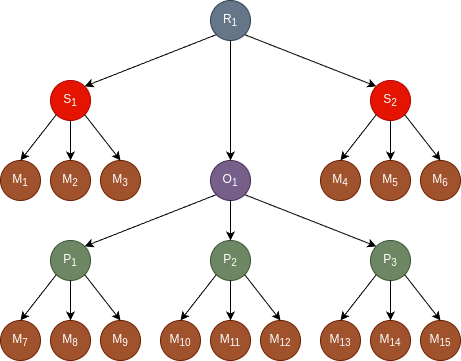
\includegraphics[scale=0.6]{../images/offline_scheduling_topology.png}
	\caption{Offline scheduling motivational example - topology}
    \label{fig:offline_scheduling_topology}
\end{figure}

\begin{figure}[!htbp]
	\centering
	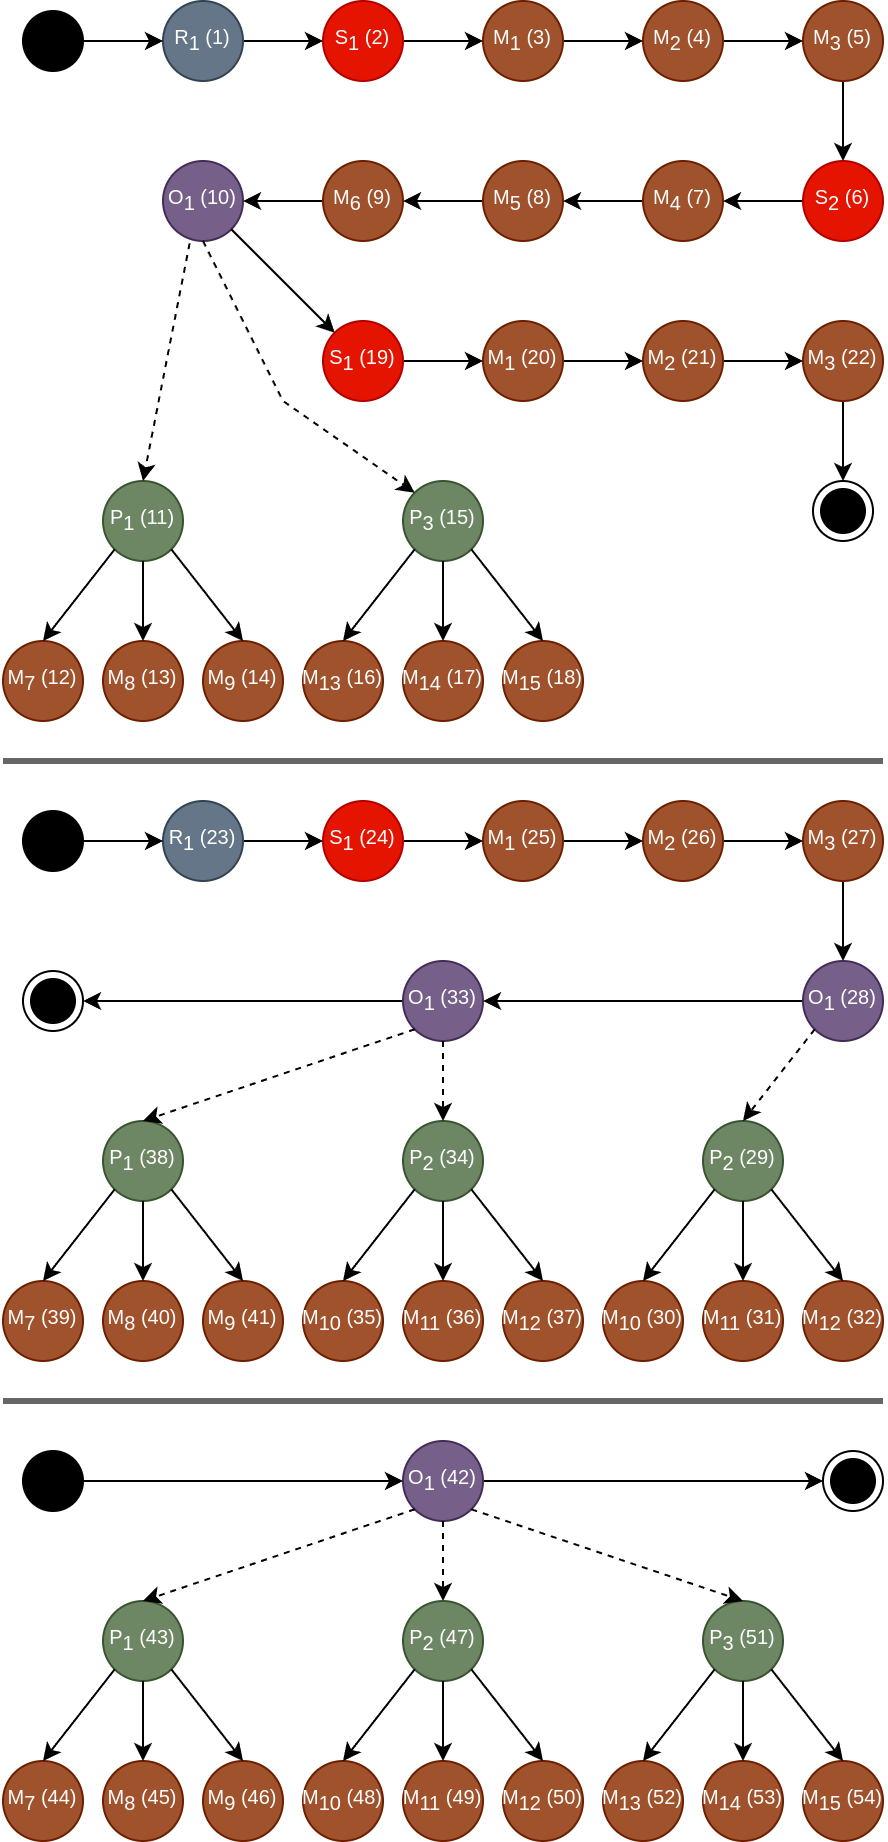
\includegraphics[scale=0.6]{../images/offline_scheduling_jobs.png}
	\caption{Offline scheduling motivational example - jobs paths DAGs}
    \label{fig:offline_scheduling_jobs}
\end{figure}

\section{Offline scheduling genotype components}
\label{sec:offline_scheduling_genotype_components}

Next, we will consider what it means to do scheduling in an environment where all information about jobs is available to the scheduler. Looking at our motivational example, we can extract some key points.

Firstly, we know the basic information about jobs - release time, due time, weight. This means that for each job, we know how important it is, when it will become available for processing, and by what time we should finish its processing.

Secondly, we know all the possible paths that each job can take through the system. We can gather this information from the job's paths DAG. In practice, this DAG would be constructed from the job's processing requirements and restrictions.

In a hierarchial topology, scheduling happens on two levels. The first one is determining a job's processing route, and the second one is determining the order in which the jobs are processed on machines.

\subsection{Offline scheduling genotype - processing routes}

First, we will focus on the processing routes. This happens in the inner nodes of the topology tree. For the serial group, no scheduling is done, as the group rules dictate that every job will be processed on the group's first component, then second, all the way to the final one. The same is true for the route group, where for each job, it is predetermined which route it will take through its components.

For the parallel group, which has of several components, and each job has to go through exactly on of them, it is the scheduler's job do decide which one the job will go through. This is the first component of an offline schedule genotype. For each job, for each path node which corresponds to a parallel group in the topology, all of its successor nodes are placed in a list, and among them one is chosen as the node the job will go through. This part of the genotype is shown in figure \ref{fig:offline_scheduling_genotype_parallel}. For three jobs, there are eight parallel group nodes, and for each them, the successor is shown in a darker color, with the remaining nodes being colored lightly.

\begin{figure}[!htbp]
	\centering
	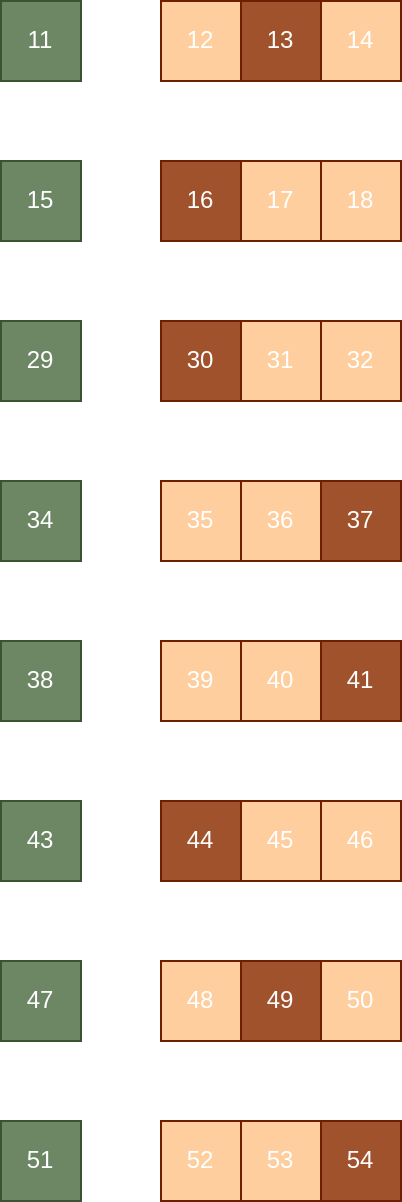
\includegraphics[scale=0.6]{../images/offline_scheduling_genotype_parallel.png}
	\caption{Offline scheduling example - genotype for parallel groups}
    \label{fig:offline_scheduling_genotype_parallel}
\end{figure}

For the open group, which also has of several components, and each job has some components it has to go through, but no restriction is imposed on the order that the job will go through them, it is the scheduler's job to determine this order. This is the second component of an offline schedule genotype. For each job, for each path node which corresponds to an open group in the topology, all of its successors are placed in a list, and the order of the components in this list dictates the order in which the job will go through the path nodes. This part of the genotype is shown in figure \ref{fig:offline_scheduling_genotype_open}. For three jobs, there are four open group nodes, and for each them, the traversal order of their successors is shown.

\begin{figure}[!htbp]
	\centering
	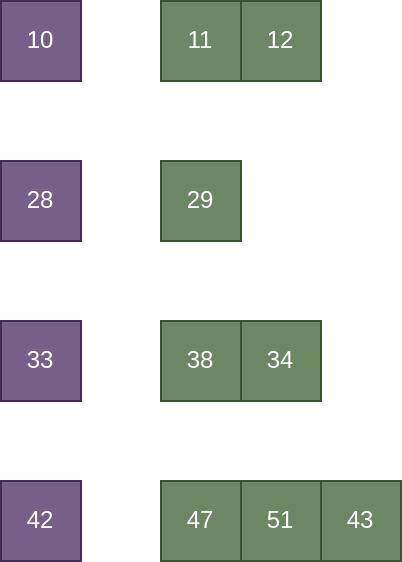
\includegraphics[scale=0.6]{../images/offline_scheduling_genotype_open.png}
	\caption{Offline scheduling example - genotype for open groups}
    \label{fig:offline_scheduling_genotype_open}
\end{figure}

\subsection{Offline scheduling genotype - processing orders}

Next, we will focus on the second level of scheduling, which is determining the order in which the jobs are processed on machines. This is the third and final component of an offline schedule genotype. For each machine, it is precalculated which processing steps can happen on it. These steps are placed in a list, and the order of this list determines the order of processing on the machine. How this works in practice is that, in the machine's buffer, jobs are ordered using the order in the genotype, and every time the machine can start processing a job, it takes the first step from the buffer and starts its processing. This part of the genotype is shown in figure \ref{fig:offline_scheduling_genotype_machine}.

\begin{figure}[!htbp]
	\centering
	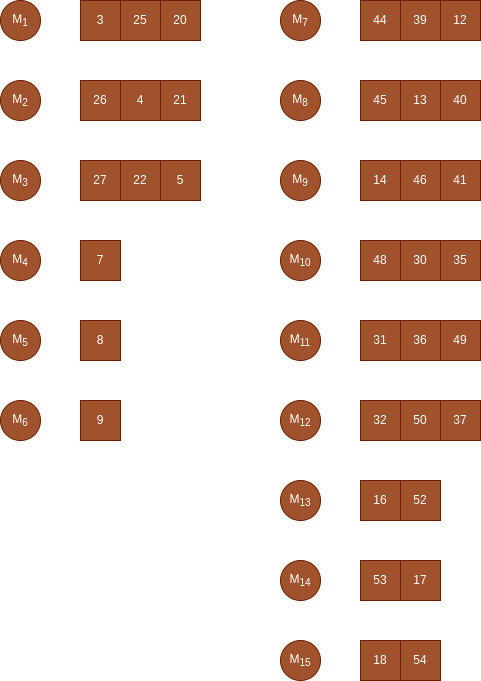
\includegraphics[scale=0.6]{../images/offline_scheduling_genotype_machine.png}
	\caption{Offline scheduling example - genotype for machines}
    \label{fig:offline_scheduling_genotype_machine}
\end{figure}

\subsection{Offline scheduling genotype - passive components}

These three components build an offline schedule genotype. An important note to make is that the genotype can contain passive components, by which we mean that they do not impact the scheduler and its decisions. 

One way that this can happen is if the topology contains parallel groups. All branches of these groups are covered by the genotype, but only one will be relevant for each job that goes through the parallel group. If a passive branch of a parallel group node contains an open group, then the order of its component nodes in the genotype will be irrelevant, until the branch becomes active by changing the parallel group node in the genotype. 

Another way in which a component of a genotype can be passive is for machines, where the genotype for each machine will be fully utilized only if all its processing steps are waiting in its buffer at the same time. Otherwise, changing the order of steps for a machine can have no impact on the order in which the steps are processed.

\section{Offline scheduling genotype operators}
\label{sec:offline_scheduling_genotype_operators}

In chapter \ref{sec:offline_scheduling_genotype_components}, we have presented the genotype for offline scheduling. In this chapter, we will present all of its operators, and this will make the offline scheduling genotype compatible and optimizable with the framework presented in chapter \ref{sec:optimization_model}.

\subsection{Offline scheduling genotype - evaluation function}
\label{sec:offline_scheduling_genotype_evaluation_function}
The evaluation model for the hierarchial topology representation was explained in chapter \ref{sec:evaluation_model}. To reiterate, the processing of a job sequence is simulated, and the simulation yields some data about each job. Then, an objective function is calculated using the job data, and the result represents the schedule score. This exactly is the evaluation function for the offline scheduling genotype - run a simulation, collect results, pass them to an objective function and calculate the schedule score. The two parameters of an evaluation function are the job sequence and the objective function, and changing them produces different evaluation functions.

\subsection{Offline scheduling genotype - creation operator}
The genotype for offline scheduling consists of three components, as described in chapter \ref{sec:offline_scheduling_genotype_components}. All genotype operators manipulate all of these components. Before the optimization, paths DAGs of all jobs are analyzed, to collect information about all possible scheduling decisions that could be made. For each machine, a list of all processing steps which could be executed on it is compiled. For parallel and open groups, all path nodes are compiled.

For machines, a creation operator constructs a random permutation of all steps which are to be executed on the machine. For parallel group nodes, a creation operator randomly chooses one of its components. For open group nodes, a creation operator constructs a random permutation of all components the job has to go through.

\subsection{Offline scheduling genotype - combination operator}
For parallel group nodes, a combination operator takes the genetic material from one of the parents. For open group nodes and machines, any combination operator for a permutation representation can be used, and several are described in \citep{cicirello2023ecta} as \textit{crossover operators}.

\subsection{Offline scheduling genotype - perturbation operator}
For parallel group nodes, a perturbation operator works in the same way as a creation operator - it randomly chooses on of the group's components. For open group nodes and machines, any perturbation operator for a permutation representation can be used, and several are described in \citep{cicirello2023ecta} as \textit{mutation operators}.

\subsection{Offline scheduling genotype - neighborhood operator}
For simple representations, a complete and exhaustive neighborhood operator can be constructed. One such representation is a binary vector representation, which consists of $n$ numbers, each one being $0$ or $1$. A neighborhood operator could flip the value at each position, and thus produce $n$ neighbors.

For more complex representations, exhaustively listing all neighbors becomes intractable. For such representations, a neighborhood operator can be simulated by using the perturbation operator $n$ times and returning all perturbations as the list of neighbors. This is the approach that we will use for the offline scheduling genotype, and all the remaining genotypes that will be explained throughout this thesis. Where a neighborhood operator is not explicitly defined, it is assumed that a perturbation operator is used as its surrogate.

\section{Topology partitioning}
\label{sec:topology_partitioning}

We have seen that an offline scheduling genotype consists of $a$ machine step permutations, $b$ parallel group node selections and $c$ open group node permutations. We have also decribed how genotype operators transform each of these genotype components. The question that is left to answer is which of these components are being transformed at any moment when an operator is being applied.

For this purpose, we will introduce the concept of topology partitioners. At certain moments during optimization, a topology partitioner will be invoked to generate a new subset of components, and only components in this subset can be altered until the next invocation of the partitioner, while the remaining components stay fixed. Next, we will describe several partitioners which we will use later.

A \textit{basic partitioner} always returns all components.

A \textit{start to end partitioner} organizes all components in a list, where the components are ordered by the topological order of their respective topology components. Each time that this partitioner is invoked, it returns $k$ components, where $k$ is a parameter which defines how many components can be changed at once. The partitioner iterates through all components from start to end with a step $k$, and when it reaches the end, it circles back to the beginning of the components list.

An \textit{end to start partitioner} works similarly to the \textit{start to end partitioner}, but it iterates through the components list from the end to the beginning. Everything else works in the same way for both partitioners.

A \textit{fair random partitioner} creates a random permutation of all components, and iterates through it from start to end with a step $k$, similarly to the \textit{start to end partitioner}. When it reaches the end of the permutation, it creates a new one. It is random because the order in which the components are changed is random, and it is fair because all components are changed roughly the same number of times.

A \textit{true random partitioner} returns $k$ random components any time it is invoked. Unlike the \textit{fair random partitioner}, there is no guarantee that components will be changed in a fair way, because they are chosen completely randomly every time that a new partition is created.

Finally, a \textit{random path partitioner} creates a random path through the topology, and returns all components on the path. When it reaches a route or open group element, it includes each of its components with a chance $p$, which is its parameter.

Next, we will discuss how the introduction of topology partitioners affects the genotype operators. The only operators which are affected are the perturbation and combination operators.

For perturbation operators, the components which are open for change are perturbated, while the remaining ones are fixed. 

For combination operators, the components which are open to change are constructed using the combination operators for the component. Since a combination operator creates a new genotype from two parent genotypes, this creates a problem in constructing new genotypes, as it is not clear how to create components which are fixed and can not be changed at the time. For this purpose, we will introduce combination operators with coarse and fine granularity. The coarse granularity operator randomly chooses a parent, and copies all fixed components from that parent. The fine granularity operator chooses a random parent for each fixed component, and copies the component from it.

\section{Scheduling meta-algorithm}
\label{sec:scheduling_meta_algorithm}

We can now describe the algorithm which we will use to do optimization for both offline and online scheduling. The algorithm is called \textit{scheduling meta-algorithm}, and its pseudocode can be found in algorithm \ref{alg:sma}.

The algorithm has two evaluation functions. The first function contains the sequence of jobs used for training, and the second function contains the sequence used for testing. This is analogous to the concepts of \textit{train sets} and \textit{test sets} in machine learning.

In the inner loop of the algorithm, an optimization algorithm searches the solution space for a good solution, evaluating the solutions on the train set. Any algorithm described in chapter \ref{sec:optimization_algorithms} can be used as the inner optimization algorithm.

In the outer loop of the algorithm, a topology partitioner is used to create a new partition of components that will be changed in the inner loop of the algorithm, the inner algorithm is called, and its result is evaluated using the test set. 

It is important to note that the population of solutions is transferred from one call of the inner algorithm to the next one. In each iteration, the topology partitioner determines which components of the genotype will be changed, while the others remain constant. This property allows the algorithm  to change only some parts of the solutions and keep the remaining ones frozen, thus exploring the solution space in a controlled way.

\begin{algorithm}[!htbp]
    \caption{Scheduling meta-algorithm}
    \label{alg:sma}
    \KwIn{$evaluation\_function\_train$, $evaluation\_function\_test$, $creation\_operator$, $combination\_operator$, $perturbation\_operator$, $topology\_partitioner$, $inner\_algorithm$, $number\_of\_iterations$}
    \KwOut{$(best\_solution, best\_score)$}

    $x \gets creation\_operator.create()$\;
    $s \gets evaluation\_function\_test.evaluate(x)$\;
    $population \gets creation\_operation.createPopulation()$\;

    \For{$iter \gets 1$ \KwTo $number\_of\_iterations$} {

        $machines\_partition = topology\_partitioner.getPartition()$\;
        $(x', \_)$ $\gets$ $inner\_algorithm.optimize($$evaluation\_function\_train,$ \newline \hspace*{1em} $creation\_operator$, $combination\_operator$,  $perturbation\_operator,$\newline \hspace*{1em}$ machines\_partition, population)$\;
        $s' \gets evaluation\_function\_test.evaluate(x')$\;
        \If{$s' < s$}{
            $(x, s) \gets (x', s')$\;
        }
    }

    \Return $(x, s)$\;
    \end{algorithm}

\section{Case study: scheduling university laboratory exercises}
\label{sec:case_study_lab}

In this chapter, we will describe how to use the offline scheduling representation to solve to problem of scheduling university laboratory exercises. The premise of the problem is that a total of $x$ students are enrolled in an university course, and they all need to pass a laboratory exercise, which is being held in $y$ different slots. The goal is to assign each student to a slot, while satisfying some constraints - each slot has a capacity of students that cannot be exceeded, and student cannot have conflicts in their university timetables.

This is an interesting problem, because it is not immediately evident how to solve this problem using the concepts explained in this chapter. But it is important to remember that scheduling is the process of allocating resources to tasks. In the model of machines and jobs, machines are resources, and jobs are tasks. In the problem of scheduling university laboratory exercises, slots are resources, and enrolled students are tasks.

Let's imagine that the exercises are organized in five different slots, three being on one day, and two being on another. On the first day, three teaching assistants are available for exercises, while on the second day, only two of them are available. Each assistant can process a maximum of ten students per slot. This means that the first three slots can have a maximum of $30$ students, while the last two can have a maximum of $20$ students. Let's also imagine that a total of 124 students are enrolled in the course.

We will also assume that the slots for exercises are defined in advance. If the slots should also be scheduled, then the problem would require scheduling on two levels - scheduling timeslots, and scheduling students to fixed timeslots. For simplicity, we will cover only the second subproblem and assume that the slots are determined by a human, which is a reasonable assumption.

For each student, we need to choose one of five available slots. This can be represented using a parallel group component. The proposed topology and paths DAG are shown in figure \ref{fig:case_study_lab}. We can assume that the machines $M_1$, $M_2$ and $M_3$ can process $30$ students in batch, while the machines $M_4$ and $M_5$ can process $20$ students.

\begin{figure}[!htbp]
	\centering
	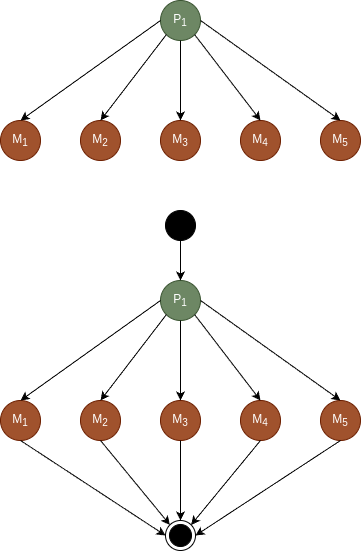
\includegraphics[scale=0.6]{../images/case_study_lab.png}
	\caption{Scheduling university laboratory exercises - topology and paths}
    \label{fig:case_study_lab}
\end{figure}

A hard constraint of the problem is that the student has no collisions in their timetable. A number of soft constraints for the problem could be defined, for example, a student does not have gaps larger than two hours in their timetable, or the student does not have to spend more than eight hours per day at university. If a solution does not satisfy a hard constraint, it is invalid. Solutions which satisfy all hard constraints can be compared in a way that those which satisfy more soft constraints are better. The goal is to ensure that no students have collisions in their timetables, and that as few students as possible have large gaps in their timetables or long days at the university.

The evaluation function would analyze the timetable of each student, and the score for a student is calculated based on whether the hard constraint is satisfied, and how many soft constraints are satisfied. Scores for all students are summed, and that is the score for the schedule.

The creation operator would randomly assign students to slots, respecting the constraints that first three slots can have no more than $30$ students, and the remaining two slots can have no more than $20$ students.

The combination operator would, for each student, randomly choose the assigned slot from one of the parents. The problem that arises is that applying this operator could break the hard constraint of the maximum number of students per slot. This can be solved by applying a greedy randomized heuristic that fixes the solution obtained from the combination operator. It would move students from the overfilled slots to the underfilled ones, using some randomized heuristic criteria.

The perturbation operator would swap the assigned slots for a randomly chosen pair of students $k$ times.

Finally, the optimization algorithm could be the \textit{scheduling meta-algorithm} if we want to utilize \textit{topology partitioners}, or any algorithm from the chapter \ref{sec:optimization_algorithms} if we want to change all slots in each iteration of the algorithm. 

In this case study, we have described, on a high level, how to use the offline scheduling representation to solve a problem of scheduling university laboratory exercises. This was an exercise of analyzing the limited resources and tasks in the problem, and applying the concepts of machines and jobs to this view of the problem. These concepts can be applied to a variety of problems, and thus, the offline scheduling representation could be used to solve such problems.

\chapter{Online scheduling model}
\label{sec:online_scheduling_model}

\section{Comparison with offline scheduling}

In this chapter, we will describe how the hierarchial topology representation can be used for solving online scheduling problems. In online scheduling, the information about jobs, such as their count and properties, is not known in advance. Instead, as the jobs enter the system, the scheduler dynamically moves them across the system.

\section{Online scheduling genotype components}
\label{sec:online_scheduling_genotype_components}

In chapter \ref{sec:offline_scheduling_model}, we have described the model for offline scheduling. The majority of the concepts presented for offline scheduling apply for online scheduling as well, including the topology partitioners and scheduling meta-algorithm. The only difference lies in how the scheduler makes decisions.

In offline scheduling, all scheduling decisions were made in advance. For each job, its path through the system was defined. For each machine, the preferred processing order of jobs was defined. In online scheduling, these decisions will be made dynamically.

\subsection{Online scheduling genotype - processing routes}

When a job is processed on a parallel machine, the scheduler needs to determine which machine the job will be processed on next. In offline scheduling, this decision is made by reading the genotype. In online scheduling, this decision is made by manipulating some features to determine the best branch of the parallel machine to enter. This problem can be framed as a classification problem. In that case, each parallel machine would have a classifier which would determine the most suitable branch.

Things get a bit more complicated when we consider online scheduling for open groups. Defining this problem as a classification problem does not make sense, because for each job, the branches of the group to select from could be different. Let's imagine that a job has $m$ components of the open group to go through. When it first arrives at the group, it is the scheduler's decision to choose which of these $m$ components the job will go through first. When the job finished with the first component, the scheduler needs to decide which of the remaining $m-1$ components the job will go through next. After that, the scheduler needs to choose one of the $m-2$ components, and this goes all the way until the job goes through all the components. So, the order of components for a job is not determined at one moment, and instead, it is constructed part by part, at different moments of the simulation.

Since framing the problem as a classification problem does not make sense for open groups, for the sake of uniformity, we will frame the problem for both parallel and open groups as a regression problem. In parallel groups, using some features, the scheduler will assign a score to each branch. The branch with the highest score is the one that the job will go through. The same applies for open groups - any time that a scheduler needs to choose which of the $k$ components a job will go through next, it will calculate a score for each of them, and the job will go through the one with the highest score. The goal of the regression algorithm is to determine how good a component of a group is, and in both the cases of parallel and open groups, the best component is chosen.

\subsection{Online scheduling genotype - processing order}

When a scheduler needs to decide which of the jobs in the machine's buffer it will process next, it will calculate the score for all of the jobs, and the job with the highest score is the one which will be processed next. The problem to solve here is a regression problem, where the goal is to determine how important a job is in the context of a machine, and the most important job gets processed first.

\section{Online scheduling features}
\label{sec:online_scheduling_features}

In chapter \ref{sec:online_scheduling_genotype_components}, we presented components of an online scheduling genotype. In offline scheduling, the genotype consists of three different categories - parallel groups, open groups and machines. In online scheduling, the genotype is more elegant. Every element of the topology which requires some form of scheduling has a regression algorithm, and the outputs of this algorithm are interpreted according to the element rules. In this chapter, we will define the features that the regression algorithms will have at their disposal to calculate the score of a job or a branch.

\subsection{Processing routes features}

For paralell and open groups, where the regression algorithm needs to evaluate how good a component of the group is for the job, the features that the algorithm can use are the following:
\begin{itemize}
    \item time (timestamp at which the job is processed on the group)
    \item job's release time
    \item job's due time
    \item job's weight
    \item job's remaining processing time in the branch
    \item the number of jobs which have entered the component
    \item the number of jobs which are currently in the component and all its descendants
    \item whether the component has free space in its buffer
    \item whether all the prerequisites for the job's processing on that component are satisfied
  \end{itemize}

\subsection{Processing order features}

For machines, where the regression algorithm needs to evaluate how important a job is relative to the machine, the features that the algorithm can use are the following:
\begin{itemize}
	\item time
	\item job's release time
	\item job's due time
	\item job's weight
	\item combined weights of all the jobs that the job is batch compatible with (can be processed in batch with)
	\item number of batch compatible jobs for the job
	\item batch processing limit (maximum number of jobs per batch) for the machine type and job type pairing
	\item setup length of the job for the machine, relative to the job which was previously processed on the machine
	\item time until the machine's next breakdown
	\item whether preemptions are allowed for the machine type and job type pairing
\end{itemize}

\section{Online scheduling limitations}
\label{sec:online_scheduling_limitations}

In this chapter, we will go over some limitations of the online scheduling model presented in this chapter.

For open groups, each time that the scheduler needs to choose the next group's component for the job, the regression algorithm for the group is executed once for each remaining component. This means that, if a job has to go through $m$ components on the open group, a total of $m + (m - 1) + (m - 2) + ... + 3 + 2$ calculations are required, which has the complexity of $O(m^2)$. This is poorly scalable, and becomes a problem if the job has a significant number of components per an open group to go through.

Similarly, for machines, each time that the scheduler needs to choose the next job to be processed on the machine, the regression algorithm for the machine is executed once for each job in the machine's buffer. If the machine's buffer can have at most $n$ jobs at any moment, and a total of $m$ jobs have to be processed on the machine, the complexity for these calculations is $O(mn)$, which is also poorly scalable.

A potential solution for this problem is to execute the regression algorithm once per component for open groups, and once per job for machines. A tradeoff is made here - processing complexity is reduced from $O(m^2)$ to $O(m)$, but the scheduler now works with outdated information. 

To remedy the problem of outdated information, an adjustment coefficient could be introduced. This would be a function of all the parameters of a regression problem. The score of a job for machines and components for open groups would become the product of the output of their respective regression algorithm and the adjustment coefficient, which could be trained in a similar way as regression algorithms. For example, for jobs in a machine's buffer, the adjustment coefficient could assign higher values to jobs which arrive earlier at the machine, thus prioritizing jobs which have waited more in the buffer.

However, in this thesis, we will not explore these concepts further, and will instead stick to the calculation models presented in the chapter \ref{sec:online_scheduling_features}. These ideas could be explored in future work.

\section{Online scheduling algorithm cluster}
\label{sec:online_scheduling_algorithm_cluster}

As we discussed earlier in this chapter, each element of the topology which requires some scheduling decisions will have a regression algorithm assigned to it. We will refer to the collection of these algorithms as the \textit{online scheduling algorithm cluster}, and a single regression algorithm will be referred to as \textit{online scheduling algorithm}.

The online scheduling algorithm cluster is the genotype for an online scheduling problem. In this chapter, we will go over its operators.

\subsection{Online scheduling algorithm cluster - evaluation function}
The evaluation function for an online scheduling algorithm cluster is the same as the evaluation function for the offline scheduling genotype, described in the chapter \ref{sec:offline_scheduling_genotype_evaluation_function}. The steps are - simulate the processing of a job sequence in the system, produce some data about each job, and aggregate this data to a single value using an objective function.

\subsection{Online scheduling algorithm cluster - creation operator}
The creation operator for an online scheduling algorithm cluster involves creating an online scheduling algorithm for each topology element that requires scheduling. This involves calling the creation operator for the online scheduling algorithm once per select topology elements.

\subsection{Online scheduling algorithm cluster - combination operator}
The combination operator for an online scheduling algorithm cluster involves calling the combination operator of the online scheduling algorithm once per topology elements unlocked by the topology partitioner, and for the topology elements which are locked by the topology partitioner, the approach which was described in chapter \ref{sec:topology_partitioning} is used, with the distinction of coarse and fine granularity combination operators.

\subsection{Online scheduling algorithm cluster - perturbation operator}
The perturbation perturbation operator for an online scheduling algorithm cluster involves calling the perturbation operator of the online scheduling algorithm once per topology elements unlocked by the topology partitioners, while the remaining elements are left intact.

\section{Online scheduling algorithms}
\label{sec:online_scheduling_algorithms}

In this chapter, we will describe the online scheduling algorithms which can make up an online scheduling algorithm cluster. An online scheduling algorithm is a genotype for solving a regression problem. In chapter \ref{sec:online_scheduling_algorithm_cluster}, we described the operators for an online scheduling algorithm cluster. The majority of these operators assume that the online scheduling algorithms have the operators of the same type defined. Based on this information, we can conclude that each online scheduling algorithm needs to have creation, combination and perturbation operators defined. Furthermore, each online scheduling algorithm needs to be able to map a set of numeric features to a number, and in this way solve a regression problem.

\subsection{Random programming}

Random programming (RP) is a simple algorithm which maps a set of features to a random number. This means that a choice of a component in a parallel group is random, the processing order of components in an open group is random, and the processing order of jobs on machines is random. It does not have any associated data structures, so all its operators are trivial. The motivation behind naming is that the majority of online scheduling algorithms which we will use will be genetic programming algorithms.

\subsection{Neural network}

Neural network (NN) \citep{nn} is an universal approximator, and in this thesis, we will limit ourselves only to feedforward networks. An illustration of a neural network is shown in figure \ref{fig:nn}. In this figure, a bias vector and a linear transformation are combined in a single affine transformation. White square elements have value $0$, gray square elements have value $1$, blue square elements correspond to a linear transformation, green square elements correspond to a bias vector, and red square element correspond to result vectors after each transformation.

The creation operator for NN creates random affine transformation matrices, and the values are generated from a normal distribution. The combination operator for NN is the arithmetic mean across all affine transformations. The perturbation operator for NN adds random Gaussian noise to all affine transformations. The regression algorithm for NN is the forward pass.

Hyperparameters for NN are the standard deviations for Gaussian distributions used in the creation and perturbation operators (mean is $0$), nonlinear activation function and the architecture of hidden layers.

\begin{figure}[!htbp]
	\centering
	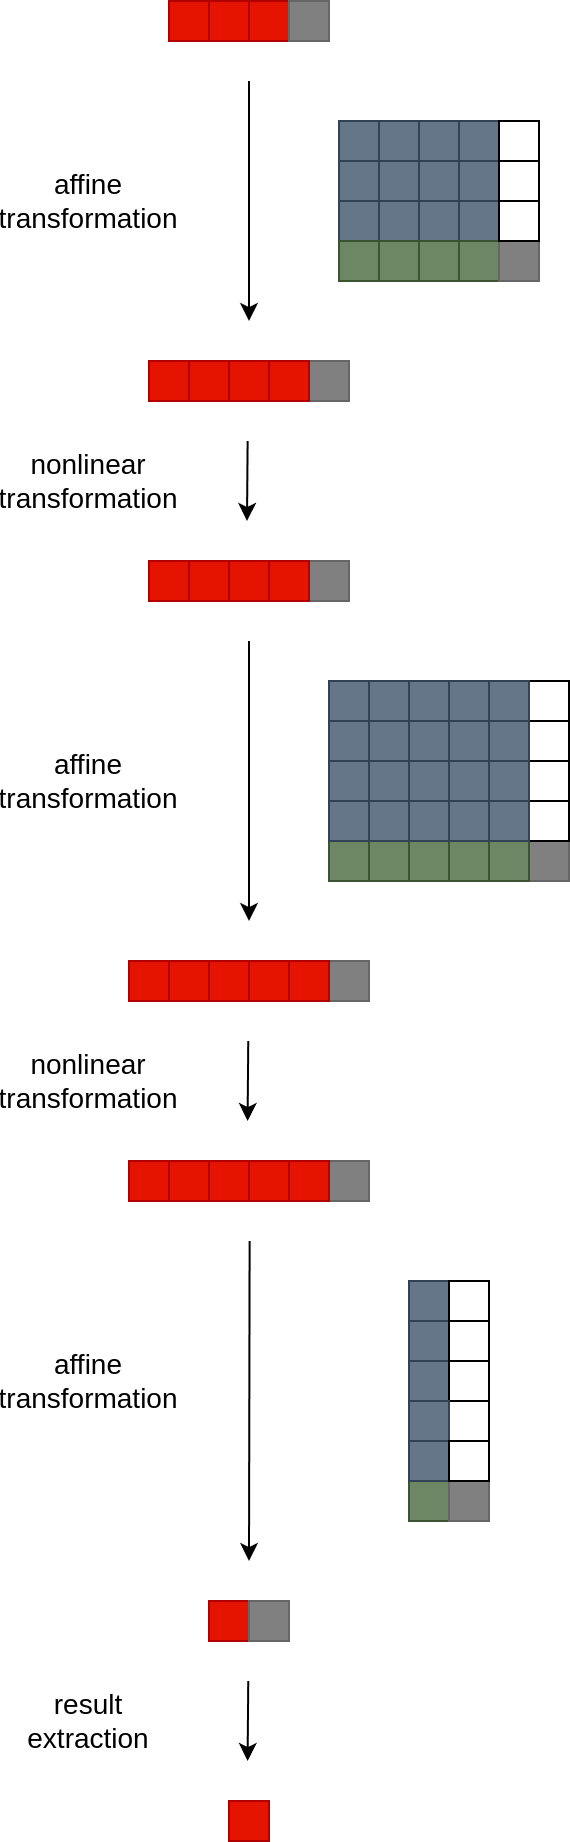
\includegraphics[scale=0.3]{../images/nn.png}
	\caption{Neural network illustration}
    \label{fig:nn}
\end{figure}

\subsection{Tree-based genetic programming}

Tree-based genetic programming (TBGP) \citep{tbgp} encodes a symbolic expression in a tree format. An illustration of TBGP for an expression for the function $x^2 + xy +2x - y$ is shown in figure \ref{fig:tbgp}. This function will be used as an example in all the remaining algorithms as well.

The creation operator creates a random tree. At each node, it has a chance of generating a parameter, a constant, or a function onde. The combination operator selects a random subtree in the first parent, and replaces it with a random subtree from the second parent. The perturbation operator selects a random subtree in the parent, and replaces it with a randomly generated subtree, which is generated using the creation operator. The regression algorithm evaluates the tree as an expression.

Hyperparameters for TBGP are the maximum height of a tree, the chance of generating a parameter leaf, and the chance of generating a constant leaf.

\begin{figure}[!htbp]
	\centering
	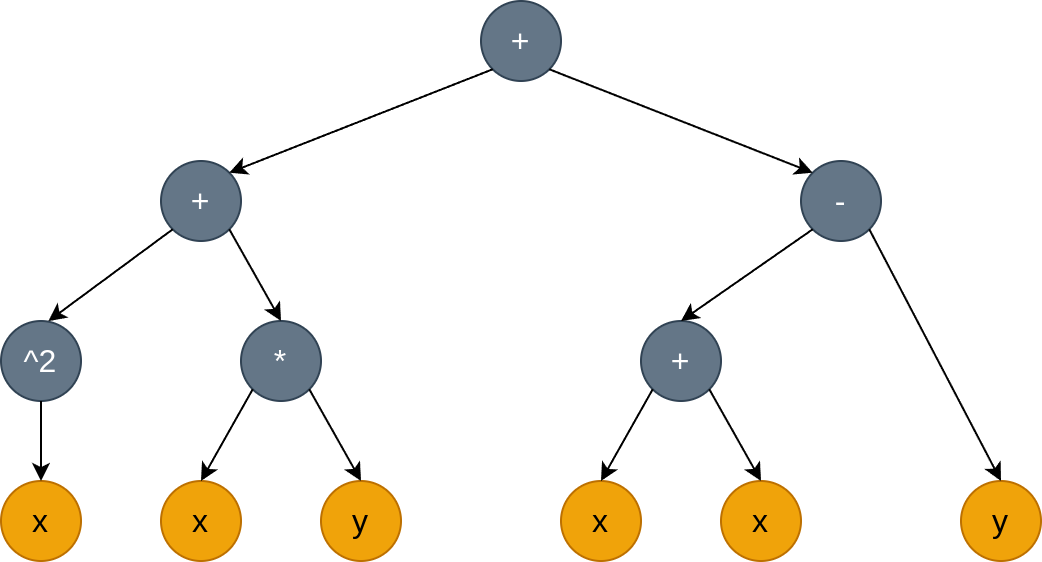
\includegraphics[scale=0.3]{../images/tbgp.png}
	\caption{Tree-based genetic programming illustration}
    \label{fig:tbgp}
\end{figure}

\subsection{Cartesian genetic programming}

Cartesian genetic programming (CGP) \citep{cgp} encodes a symbolic expression in a two-dimensional grid of function nodes. Since functions may not have the same arity, each node has the number of arguments which is equal to the maximum arity across all functions. The output of the grid can be chosen as any of the grid elements, or any of the inputs. An illustration of CGP is shown in figure \ref{fig:cgp}.

The creation operator creates a random grid. The combination operator generates a random breakpoint in the grid, and it copies the part from the start to the breakpoint from the first parent, and the part from the breakpoint to the end from the second parent. This scheme is often called \textit{one-point crossover}. The mutation operator selects $k$ random nodes, and either changes their function, or their arguments. The regression algorithm evaluates all grid elements, column by column, and the output is taken from the output node. This algorithm can be optimized using top-down dynamic programming.

Hyperparameters for CGP are the number of rows, number of columns, and the perturbation rate, which encodes the percentage of grid nodes which will be changed by the perturbation operator.

\begin{figure}[!htbp]
	\centering
	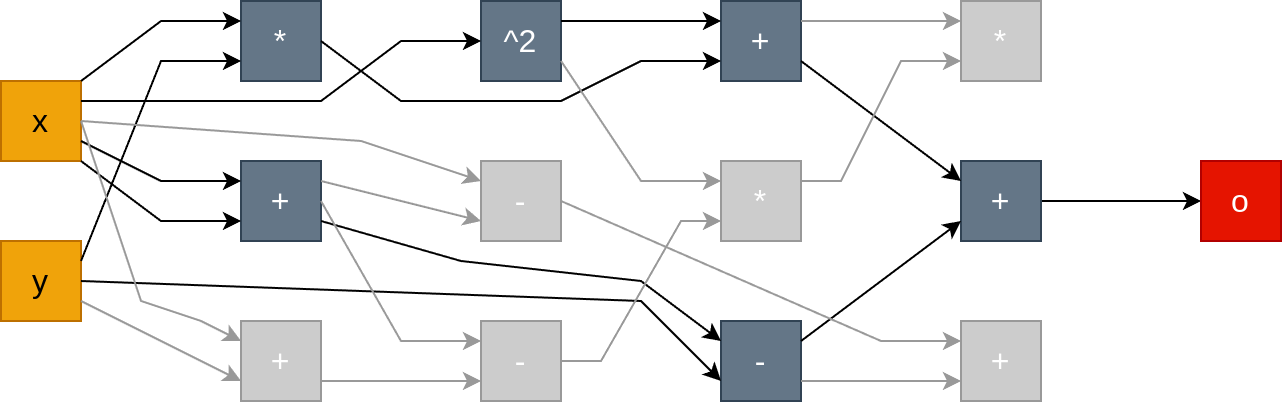
\includegraphics[scale=0.3]{../images/cgp.png}
	\caption{Cartesian genetic programming illustration}
    \label{fig:cgp}
\end{figure}

\subsection{Graph-based genetic programming}

Graph-based genetic programming (GBGP) encodes a symbolic expression in a directed acylcic graph. An illustration of GBGP is shown in figure \ref{fig:gbgp}. Representation and perturbation operator for GBGP were derived from \citep{gbgp}, while the combination operator for GBGP was derived from \citep{gbgp_operators}.

The creation operator creates a random graph. The combination operator selects a random subgraph in the first parent, and replaces it with a random subgraph from the second parent. The perturbation operator deletes a random amount of nodes, inserts a random amount of nodes, and changes either the function or the arguments for a random amount of nodes. The regression algorithm evaluates the expression encoded in the graph, and is very similar to the regression algorithm for CGP.

Hyperparameters for GBGP are the maximum number of nodes, perturbation rate, maximum number of nodes to delete during perturbation, maximum number of nodes to insert during perturbation, maximum number of nodes to crossover during combination, and the chance of proceeding to a predecessor of a node, which is used when selecting subgraphs during combination.

\begin{figure}[!htbp]
	\centering
	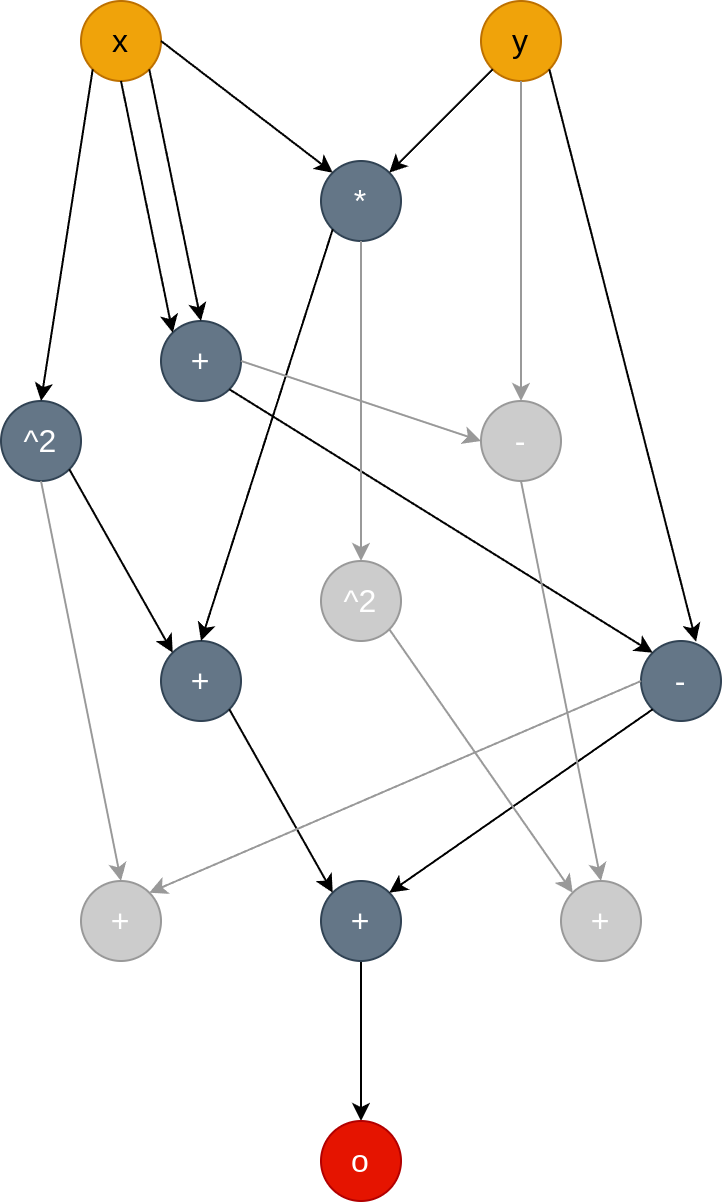
\includegraphics[scale=0.3]{../images/gbgp.png}
	\caption{Graph-based genetic programming illustration}
    \label{fig:gbgp}
\end{figure}

\subsection{Stack-based genetic programming}

Stack-based genetic programming (SBGP) \citep{sbgp} encodes a symbolic expression in the Reverse Polish Notation (RPN). A few rules are needed to ensure that the program execution is always valid. If the top element of the stack is a function, and it does not have enough arguments on the stack, then it is removed from the stack without any further manipulations. If the stack is empty when the evaluation finishes, then the value $0$ is returned instead of an error. An illustration of SBGP is shown in figure \ref{fig:sbgp}. The set of instructions is shown on the left, and the state of the stack after each operation is shown on the right of the figure. The number of instructions is fixed, and empty instructions are encoded as \textit{NOP (no operation)}, to functionally allow programs to have different lengths.

The creation operator creates a random expression in RPN. The combination operator is the one-point crossover. The perturbation operator randomly selects some functions and replaces them with different functions. The regression algorithm evaluates the expression using a stack.

Hyperparameters for SBGP are the number of instructions, chance of \textit{NOP} during creation, chance of \textit{NOP} during perturbation, the chance of generating a \textit{PUSH <constant>} instruction, the chance of generating a \textit{PUSH <parameter>} instruction, and the perturbation rate.

\begin{figure}[!htbp]
	\centering
	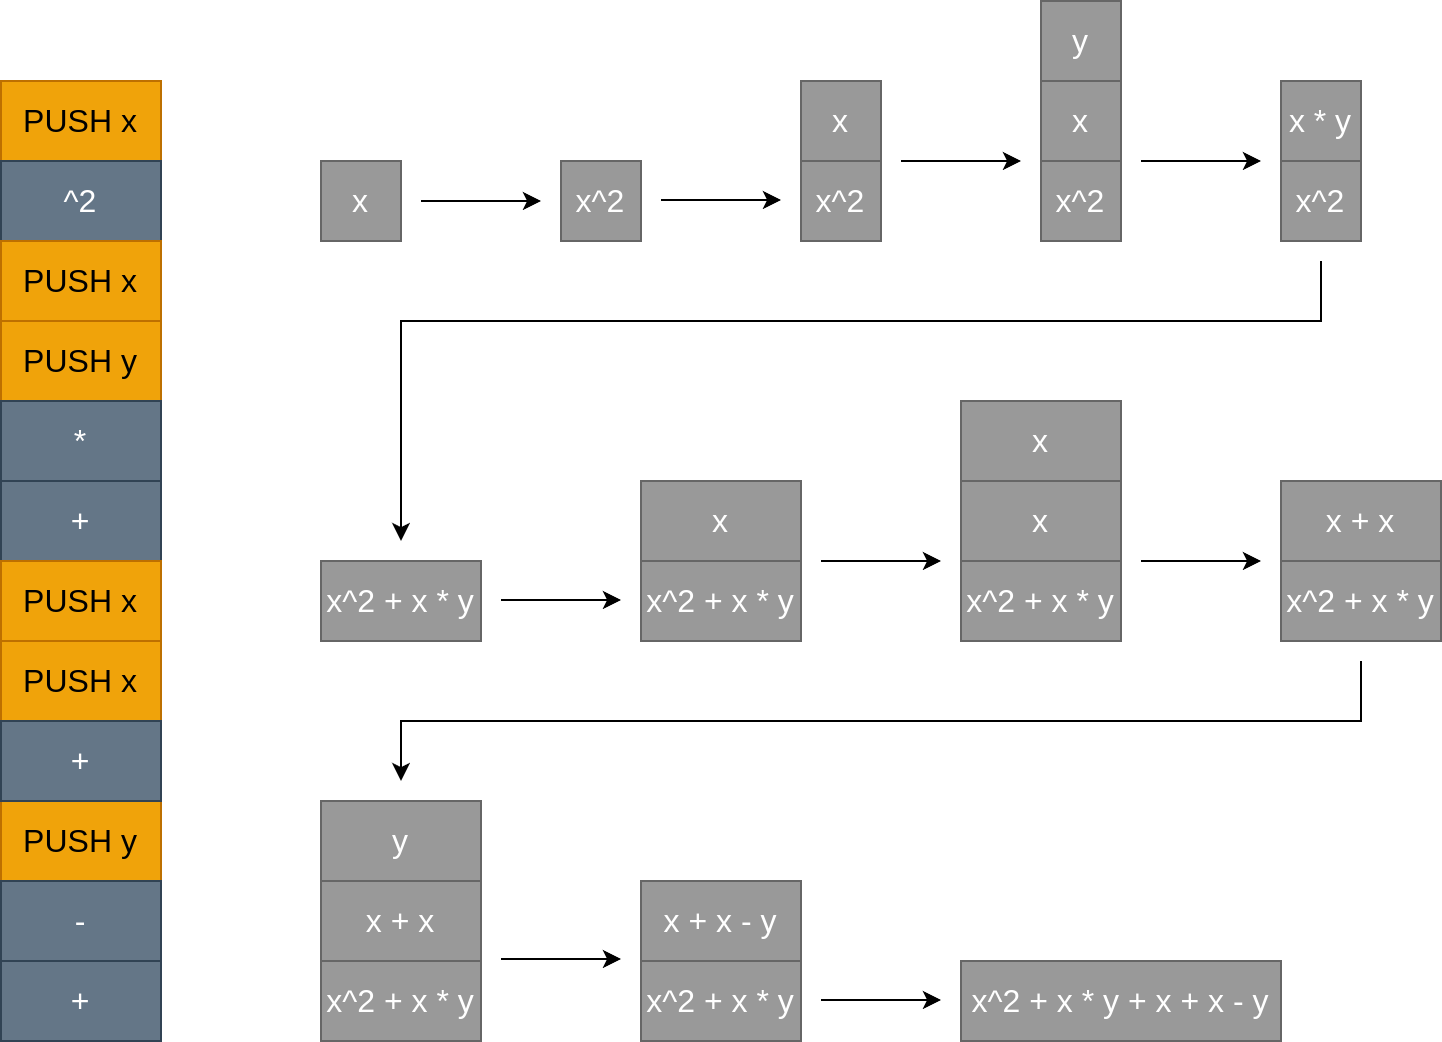
\includegraphics[scale=0.28]{../images/sbgp.png}
	\caption{Stack-based genetic programming illustration}
    \label{fig:sbgp}
\end{figure}

\subsection{Linear genetic programming}

Linear genetic programming (LGP) \citep{lgp} encodes a symbolic expression in an imperative program, containing instructions which resemble a RISC architecture. Similar to SBGP, programs have a fixed number of instructions, but some of these instructions can be empty \textit{NOP} instructions. An illustration of LGP is shown in figure \ref{fig:lgp}. The set of instructions is shown on the left, and the state of registers after each operation is shown on the right.

The program has a fixed number of registers to work with. Registers can be initialized in several ways:
\begin{itemize}
	\item empty - all registers are initialized to zero
	\item singular - first $k$ registers are initialized to $k$ parameters, and the remaining registers are initialized to zero
	\item circular - all registers are initialized in a round-robin way, using parameters
\end{itemize}

The creation operator creates a random program. The combination operator is the one-point crossover. The perturbation operator randomly selects some instructions and changes either their type or their arguments. The regression algorithm executes the program and returns the value in the first register.

Hyperparameters for LGP are the number of instructions, number of registers, register initialization strategy, chance of \textit{NOP} during creation, chance of \textit{NOP} during perturbation and the perturbation rate.

\begin{figure}[!htbp]
	\centering
	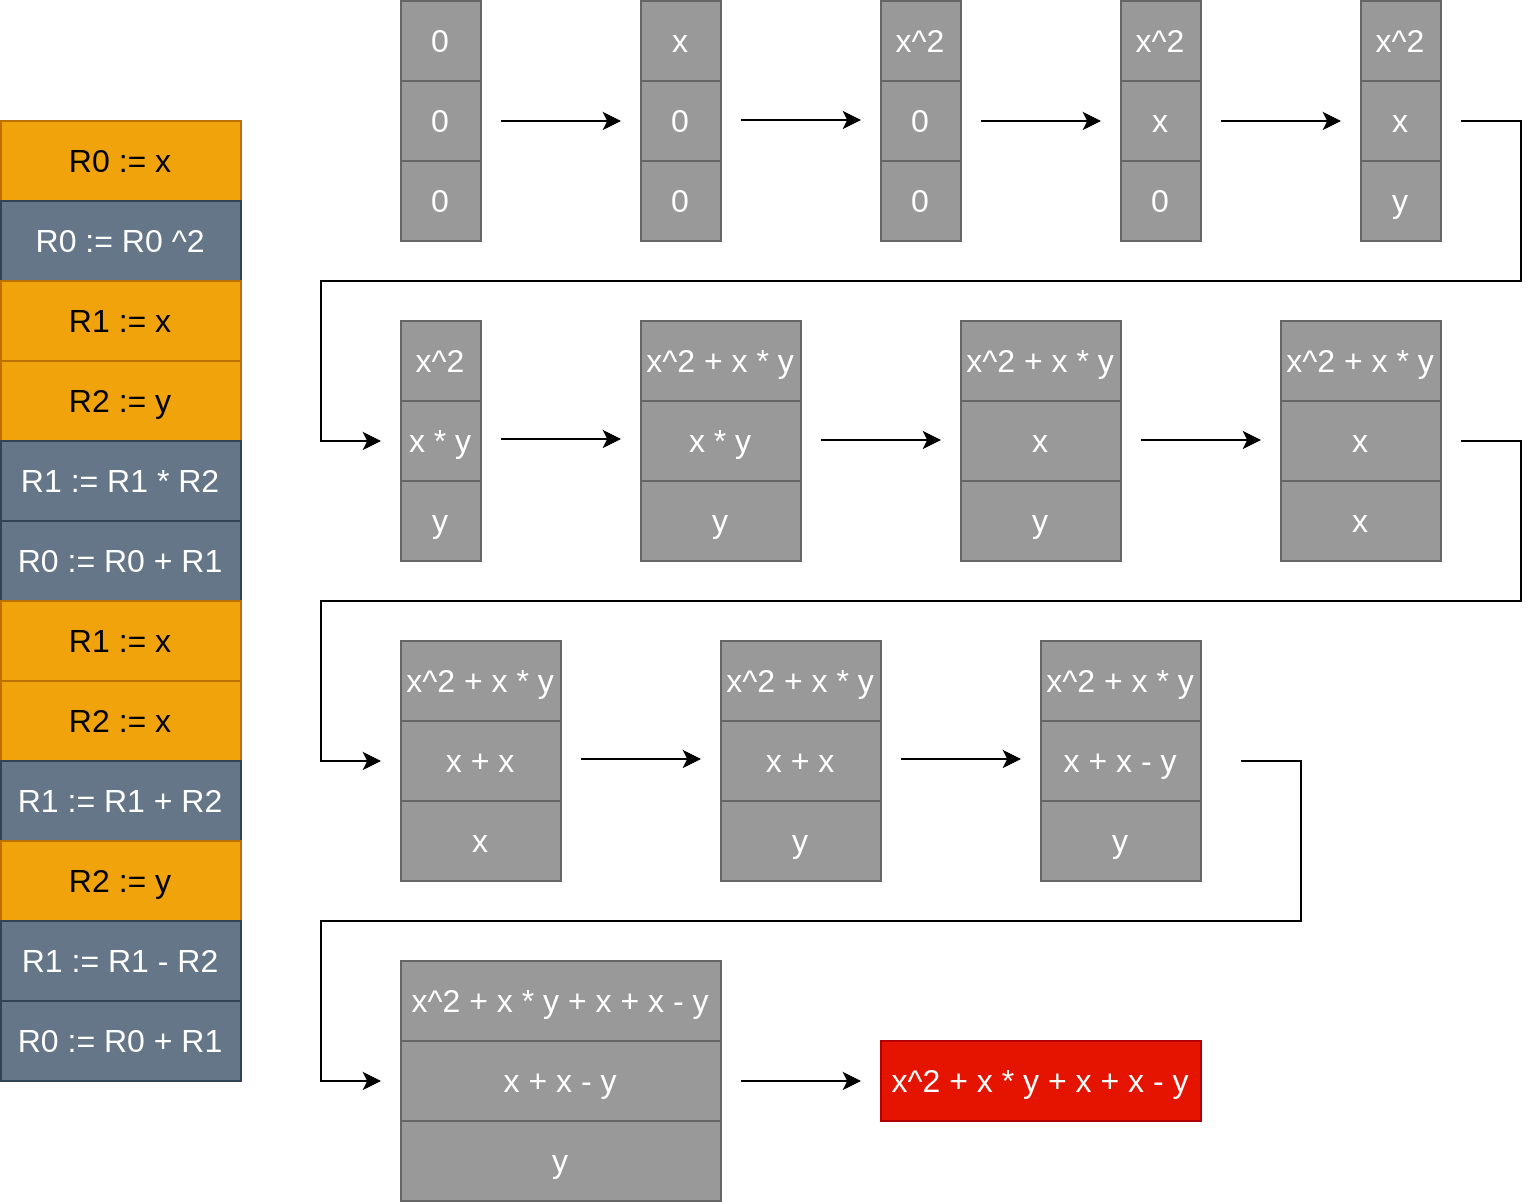
\includegraphics[scale=0.25]{../images/lgp.png}
	\caption{Linear genetic programming illustration}
    \label{fig:lgp}
\end{figure}

\subsection{Multi expression programming}

Multi expression programming (MEP) \citep{mep} encodes several symbol expressions, where expressions are built using the previous expressions, and any one of them can be used as the solution for the problem. To adapt this algorithm to be usable for online scheduling, we will always use the last expression as the result for the regression problem. An illustration of MEP is shown in figure \ref{fig:mep}.

The creation operator creates a random program. The combination operator is the one-point crossover. The perturbation operator randmoly selects some expressions and changes their arguments or function. The regression algorithm evaluates all expressions and uses the last one as the result.

Hyperparameters for MEP are the number of instructions and the perturbation rate.

\begin{figure}[!htbp]
	\centering
	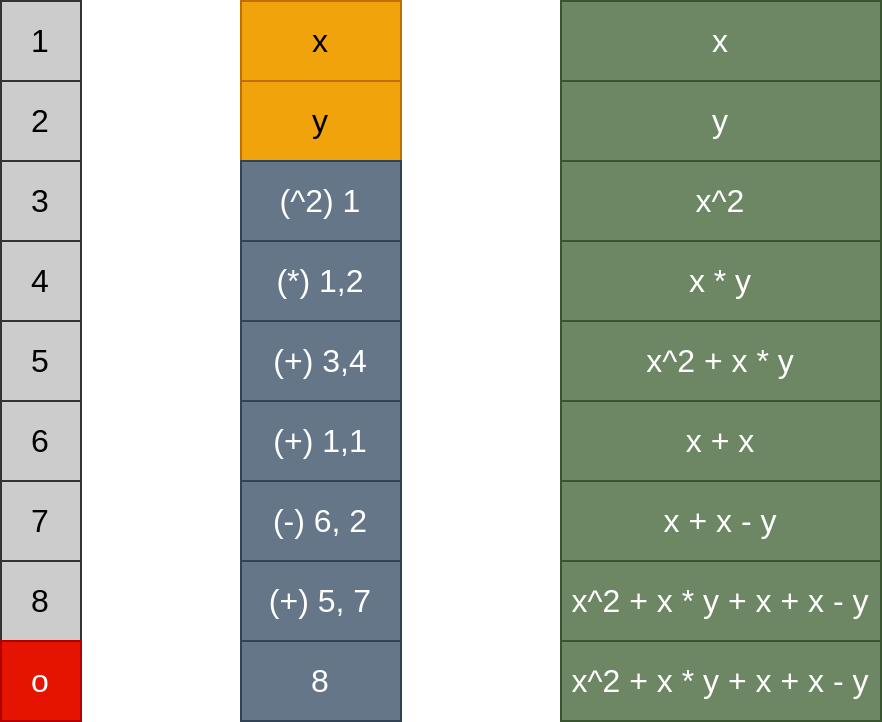
\includegraphics[scale=0.3]{../images/mep.png}
	\caption{Multi expression programming illustration}
    \label{fig:mep}
\end{figure}

\subsection{Gene expression programming}

Gene expression programming (GEP) \citep{gep} has distinct representations for its genotype and phenotype. The genotype is a linear string of elements, which can be either function symbols, parameters or constants. The phenotype is constructed by using the genotype to build the expression tree, level by level. The genotype consists of two parts, head and tail. The head can contain function symbols, while the tail cannot. The length of the head is a hyperparameter of the algorithm, and the length of the tail is calculated from the head's length. This ensures that the resulting expression is always valid and complete. And illustration of GEP is shown in figure \ref{fig:gep}.

The creation operator creates a random genotype string. The combination operator is the one-point crossover. The perturbation operator randomly selects some genotype elements and changes them, and also randomly performs transposition, which selects a segment of the genotype, and moves it to a different position within the genotype. The regression algorithm build the phenotype tree from the genotype, and then evaluates the expression encoded in the tree.

Hyperparameters for GEP are the head size, the chance of generating a parameter in the tail (as opposed to a constant), perturbation rate, chance of transposition happening in perturbation, and the maximum length of the segment in the transposition.

\begin{figure}[!htbp]
	\centering
	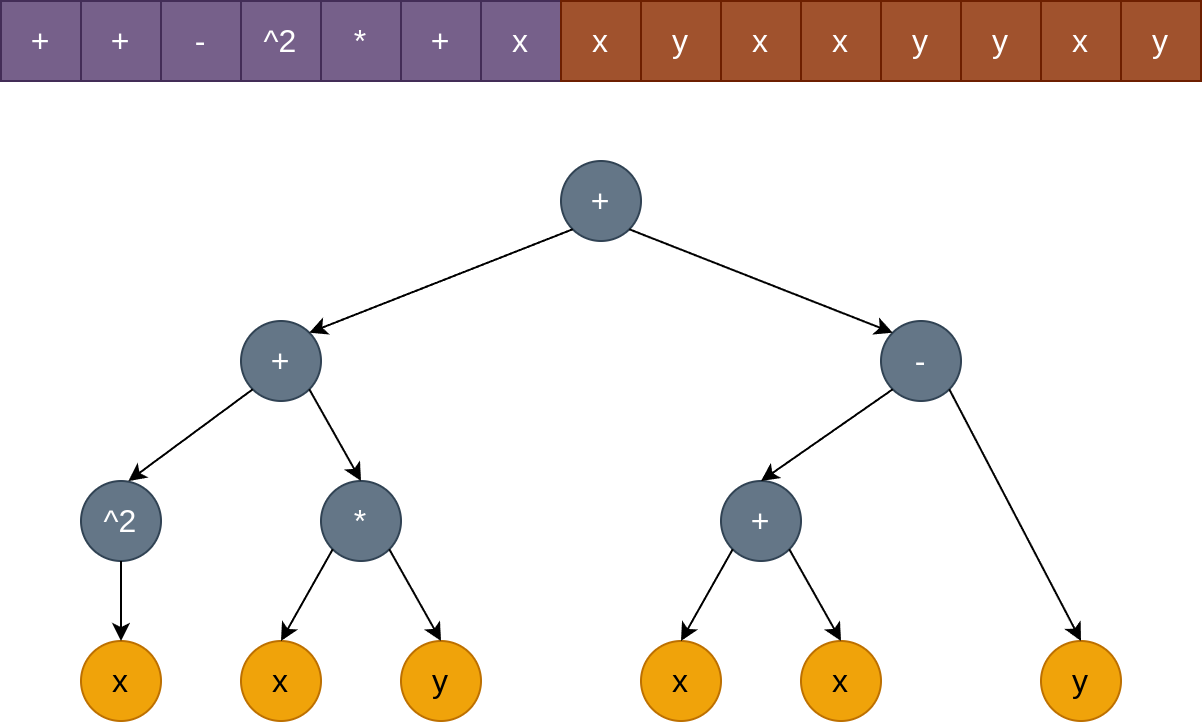
\includegraphics[scale=0.3]{../images/gep.png}
	\caption{Gene expression programming illustration}
    \label{fig:gep}
\end{figure}

\subsection{Grammatical evolution}

Grammatical evolution (GE) \citep{ge} is another algorithm with distinct representations for genotype and phenotype. The genotype is a linear string of integers called codons, and the phenotype is an expression tree. The phenotype tree is constructed from the genotype string using a context-free grammar and the modulo operator. Each time that a production is used, one codon is consumed. When all codons are consumed, the mapping starts from the beginning, and this process is called wrapping. The number of wrappings should be limited. In some cases, the mapping from genotype to phenotype may not be successful, for example due to loops. In this case, the authors of the algorithm propose assigning the lowest possible fitness value to the individual. However, this is not applicable in the case of scheduling, where it takes several evaluations of an online scheduling algorithm before the whole system can be evaluated. Instead, if the phenotype construction fails, the algorithm will always return a constant value $0$. An illustration of GE is shown in figure \ref{fig:ge}.

The creation operator creates a random genotype string. The combination operator is the one-point crossover. The perturbation operator randomly selects some codons and changes their values. The regression algorithm builds the phenotype tree from the genotype, and then evaluates it as an expression.

Hyperparameters for GE are the codon count, the maximum number of wrappings, and the perturbation rate.

\begin{figure}[!htbp]
	\centering
	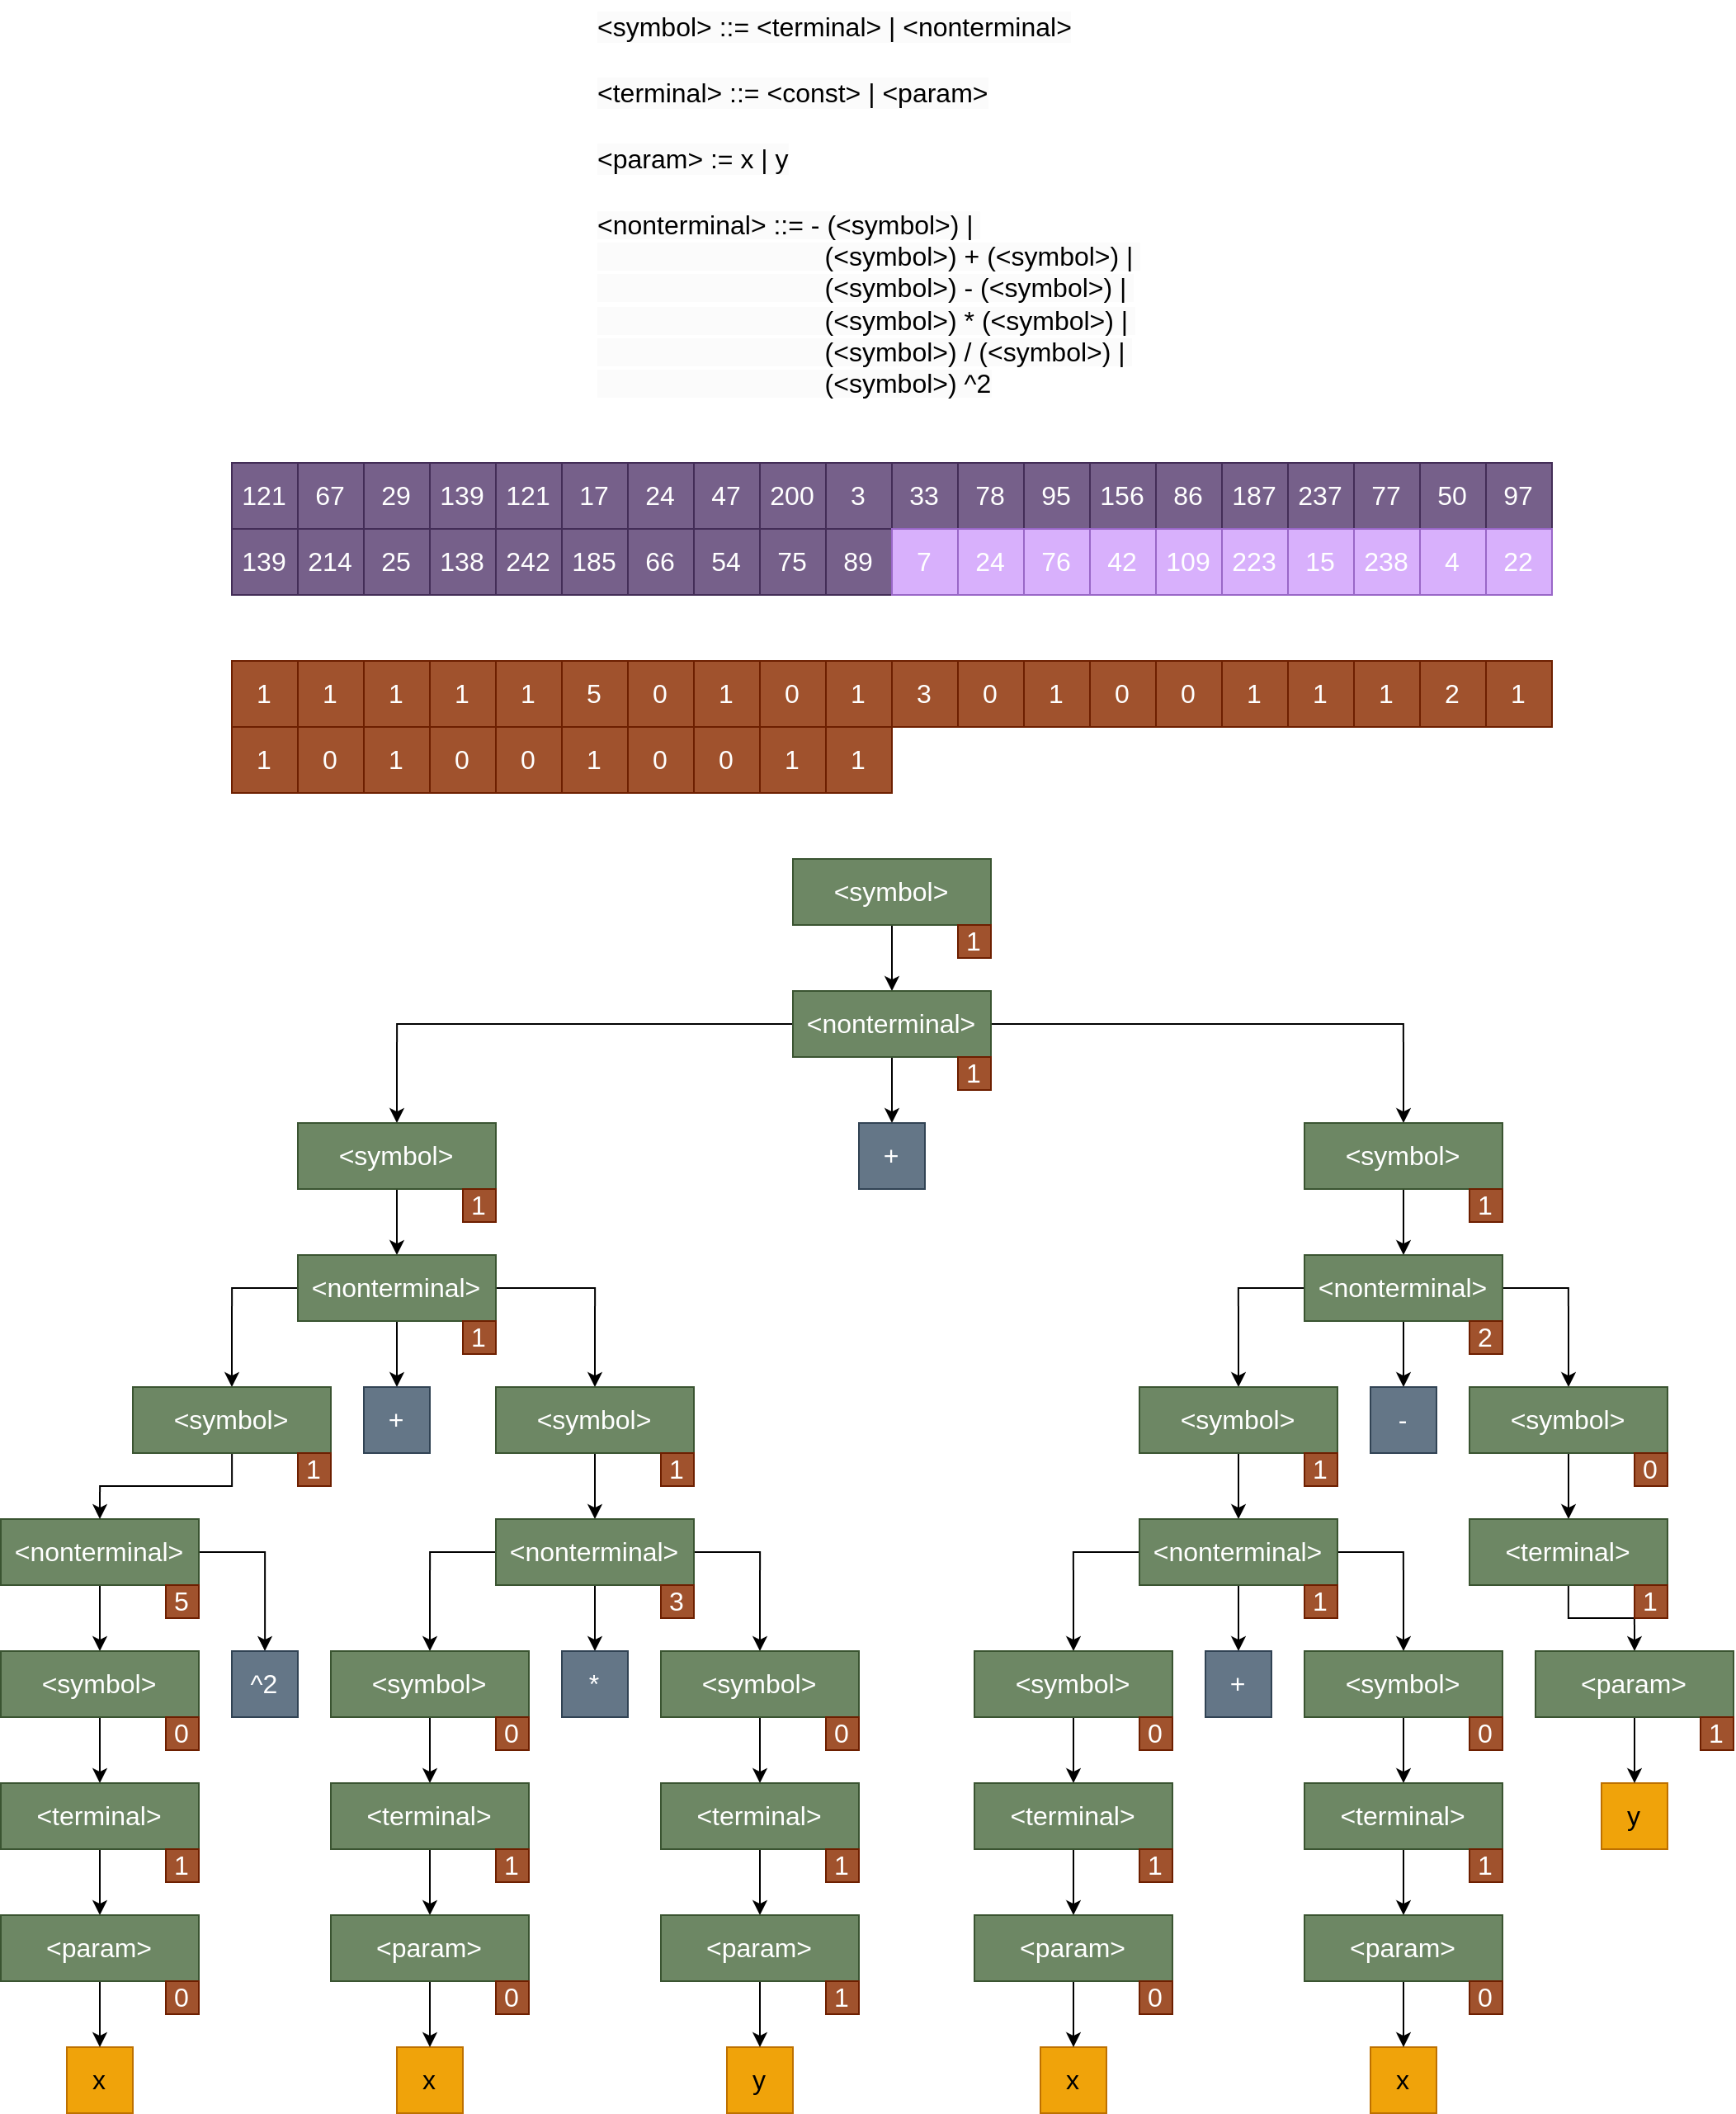
\includegraphics[scale=0.19]{../images/ge.png}
	\caption{Grammatical evolution illustration}
    \label{fig:ge}
\end{figure}

\subsection{Structured grammatical evolution}

Structured grammatical evolution (SGE) \citep{sge} is an algorithm inspired by the GE. It solves the problem of the mapping from genotype to phenotype possibly failing, by limiting the depth of the tree. For each nonterminal symbol in the grammar, it keeps a linear string of codons, whose length is equal to the maximum number of times that a symbol could appear in any tree, with the given maximum depth. An illustration of SGE is shown in figure \ref{fig:sge}. The maximum depth here is three, and the source of the recursion in the grammar is the $symbol$ node being mapped to a combination of $nonterminal$ nodes and an operator. In this case, after this transformation is applied three times in any path from the root of the tree to its leaves, the $symbol$ node will always be mapped to the $terminal$ node, thus ending the recursion.

The creation operator creates random genotype strings, one for each nonterminal symbol. The combination operator follows this procedure for each nonterminal symbol - choose a random parent, and copy its genotype for the nonterminal symbol to the child. The perturbation operator randomly selects some codons and changes their values. The regression algorithm build the phenotype tree from the genotype, and then evaluates it as an expression.

Hyperparameters for SGE are the maximum depth and the perturbation rate.

\begin{figure}[!htbp]
	\centering
	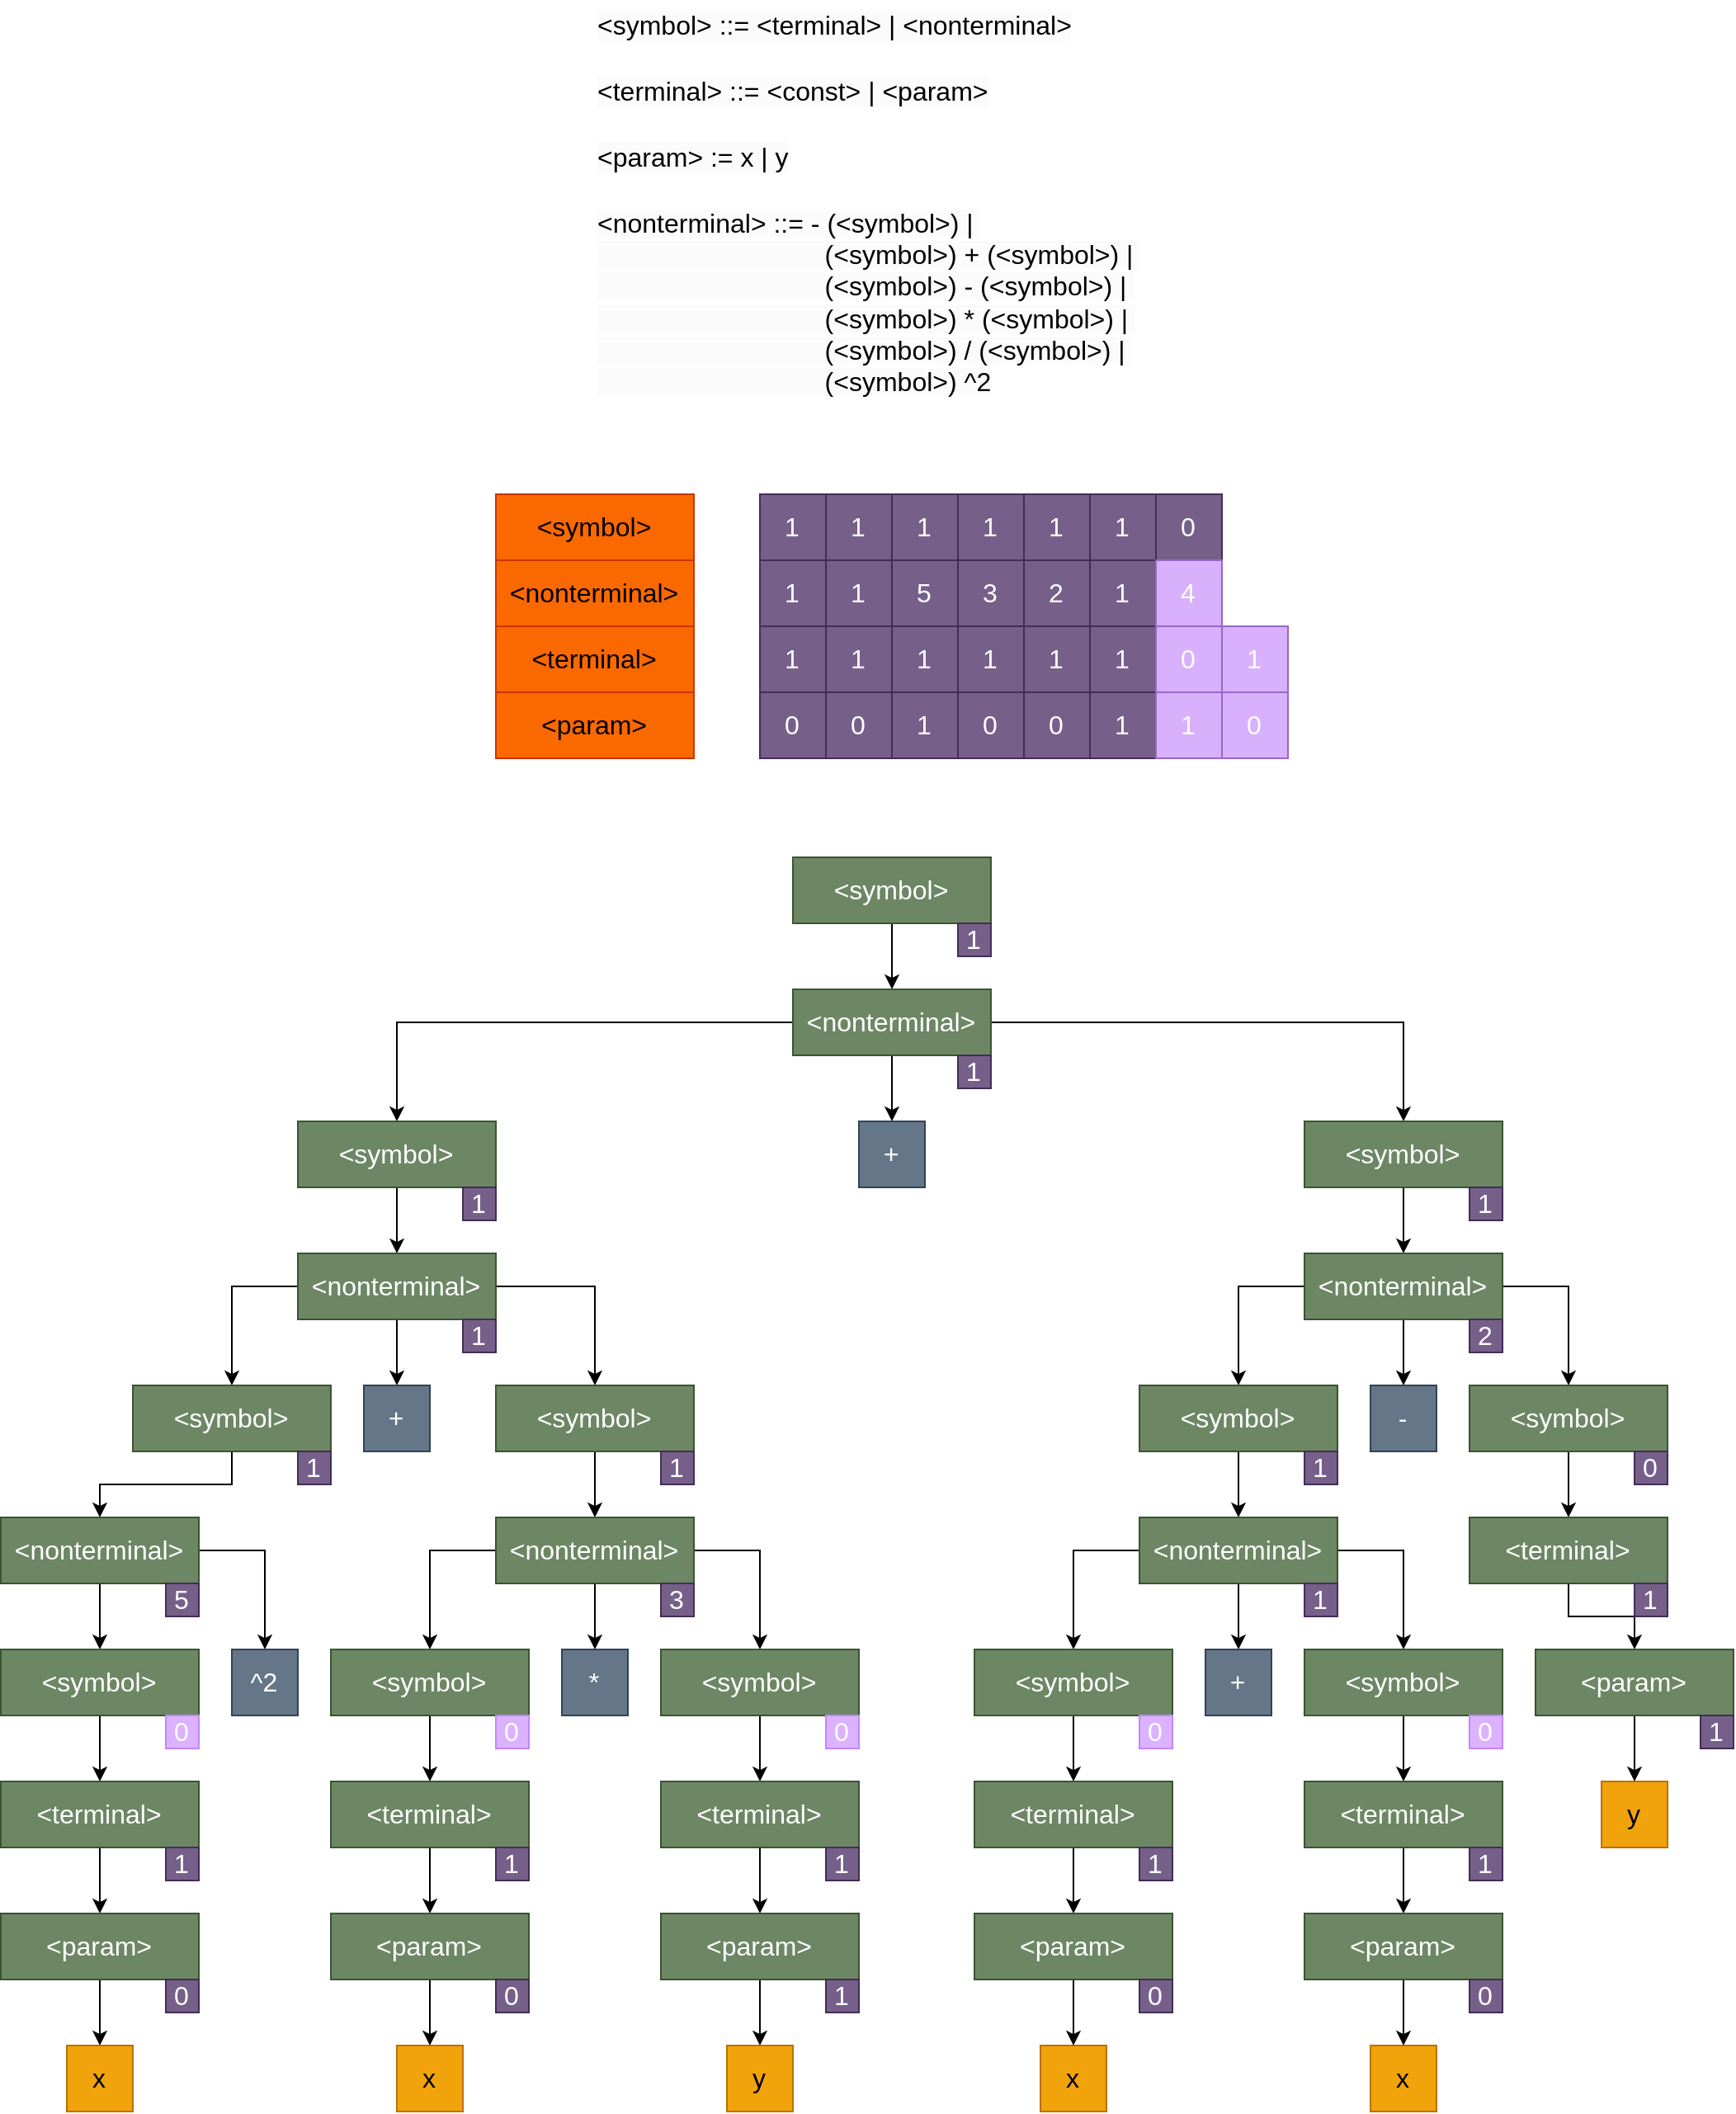
\includegraphics[scale=0.19]{../images/sge.png}
	\caption{Structured grammatical evolution illustration}
    \label{fig:sge}
\end{figure}

\chapter{Experiments and results}
\label{sec:experiments_and_results}
\section{Experimental settings}
\section{Hyperparameter tuning}

The online scheduling algorithm cluster genotype has a handful of hyperparameters. They are all shown in the table \ref{tab:hyper_all}, along with their values which we will consider. One of the hyperparameters is the optimization algorithm which is used for training, and each algorithm has several hyperparameters.

For the topology partitioner scheme, the number $k$ is calculated as the mathematical round of the square root of the total number of elements in the topology which require an online scheduling algorithm.

\begin{table}[!htbp]
    \begin{center}
        \begin{tabular}{|>{\raggedright\arraybackslash}p{0.3\linewidth}|>{\raggedright\arraybackslash}p{0.6\linewidth}|} 
         \hline
            Hyperparameter & Values \\ [0.5ex] \hline\hline
            cluster combination operator granularity & coarse, fine \\
            \hline
            topology partitioner scheme & all, 1 beginning, 1 end, 1 fair random, 1 true random, k beginning, k end, k fair random, k true random, random path \\
            \hline
            random path topology enumerator change element chance & 0.5, 0.6, 0.7, 0.8, 0.9 \\
            \hline
            optimization algorithm & SSGA, GGA, ES, SIA, CLONALG \\
            \hline
            SSGA population size & 5, 10, 15, 20 \\
            \hline
            SSGA evaluations in inner algorithm & 100, 50, 25, 20 \\
            \hline
            GGA population size & 5, 10, 15, 20 \\
            \hline
            GGA evaluations in inner algorithm & 100, 50, 25, 20 \\
            \hline
            GGA worst unit coefficient & 0.1, 0.2, 0.3, 0.4, 0.5 \\
            \hline
            ES population size & 5, 10, 15, 20 \\
            \hline
            ES evaluations in inner algorithm & 100, 50, 25, 20 \\
            \hline
            ES new units per generation percentage & 0.05, 0.1, 0.15, 0.2, 0.3, 0.4, 0.5 \\
            \hline
            SIA population size & 5, 10, 15, 20 \\
            \hline
            SIA evaluations in inner algorithm & 100, 50, 25, 20 \\
            \hline
            SIA number of clones per individual & 1, 2, 3, 4, 5 \\
            \hline
            CLONALG population size & 5, 10, 15, 20 \\
            \hline
            CLONALG evaluations in inner algorithm & 100, 50, 25, 20 \\
            \hline
            CLONALG $\beta$ & 0.1, 0.2, 0.3, 0.4, 0.5 \\
            \hline
            CLONALG $\gamma$ & 0.05, 0.1, 0.15, 0.2 \\
            \hline
            CLONALG $\lambda$ & 3, 5, 8, 10 \\
            \hline
        \end{tabular}
    \end{center}
    \caption{Hyperparameter values - all algorithms}
\label{tab:hyper_all}
\end{table}

Furthermore, the online scheduling algorithm cluster has an additional parameter, which is the online scheduling algorithm it employs for all regression problems. Each online scheduling algorithm has several hyperparameters. They are shown in the following tables - NN in table \ref{tab:hyper_nn}, TBGP in table \ref{tab:hyper_tbgp}, CGP in table \ref{tab:hyper_cgp}, GBGP in table \ref{tab:hyper_gbgp}, SBGP in table \ref{tab:hyper_sbgp}, LGP in table \ref{tab:hyper_lgp}, MEP in table \ref{tab:hyper_mep}, GEP in table \ref{tab:hyper_gep}, GE in table \ref{tab:hyper_ge} and SGE in table \ref{tab:hyper_sge}.

\begin{table}[!htbp]
    \begin{center}
        \begin{tabular}{|>{\raggedright\arraybackslash}p{0.3\linewidth}|>{\raggedright\arraybackslash}p{0.6\linewidth}|} 
         \hline
            Hyperparameter & Values \\ [0.5ex] \hline\hline
            creation $\sigma$ & 0.001, 0.01, 0.1, 1.0 \\
            \hline
            perturbation $\sigma$ & 0.001, 0.01, 0.1, 1.0 \\
            \hline
            activation function & sigmoid, ReLU, tanh, leaky ReLU \\
            \hline
            hidden layers & $-$, $5$, $10$, $20$, $10 \times 5$, $10 \times 10$, $20 \times 10$, $20 \times 20$, $10 \times 10 \times 5$, $20 \times 10 \times 5$, $20 \times 20 \times 20$, $20 \times 15 \times 10 \times 5$ \\
            \hline
        \end{tabular}
    \end{center}
    \caption{Hyperparameter values - NN}
\label{tab:hyper_nn}
\end{table}

\begin{table}[!htbp]
    \begin{center}
        \begin{tabular}{|>{\raggedright\arraybackslash}p{0.3\linewidth}|>{\raggedright\arraybackslash}p{0.6\linewidth}|} 
         \hline
            Hyperparameter & Values \\ [0.5ex] \hline\hline
            maximum height & 5, 8, 10, 12, 15 \\
            \hline
            constant leaf chance & 0.05, 0.1, 0.15, 0.2\\
            \hline
            parameter leaf chance & 0.1, 0.2, 0.3, 0.4, 0.5 \\
            \hline
        \end{tabular}
    \end{center}
    \caption{Hyperparameter values - TBGP}
\label{tab:hyper_tbgp}
\end{table}

\begin{table}[!htbp]
    \begin{center}
        \begin{tabular}{|>{\raggedright\arraybackslash}p{0.3\linewidth}|>{\raggedright\arraybackslash}p{0.6\linewidth}|} 
         \hline
            Hyperparameter & Values \\ [0.5ex] \hline\hline
            number of rows & 3, 5, 8, 10, 15 \\
            \hline
            number of columns & 3, 5, 8, 10, 15 \\
            \hline
            perturbation rate & 0.05, 0.1, 0.2, 0.3 \\
            \hline
        \end{tabular}
    \end{center}
    \caption{Hyperparameter values - CGP}
\label{tab:hyper_cgp}
\end{table}

\begin{table}[!htbp]
    \begin{center}
        \begin{tabular}{|>{\raggedright\arraybackslash}p{0.3\linewidth}|>{\raggedright\arraybackslash}p{0.6\linewidth}|} 
         \hline
            Hyperparameter & Values \\ [0.5ex] \hline\hline
            maximum number of nodes & 20, 50, 100, 150, 200, 300 \\
            \hline
            perturbation rate & 0.05, 0.1, 0.2, 0.3 \\
            \hline
            maximum nodes to delete & 1, 2, 3, 4, 5 \\
            \hline
            maximum nodes to insert & 1, 2, 3, 4, 5 \\
            \hline
            maximum nodes in crossover & 5, 10, 15, 20 \\
            \hline
            exchange branch in crossover chance & 0.5, 0.6, 0.7, 0.8, 0.9 \\
            \hline
        \end{tabular}
    \end{center}
    \caption{Hyperparameter values - GBGP}
\label{tab:hyper_gbgp}
\end{table}

\begin{table}[!htbp]
    \begin{center}
        \begin{tabular}{|>{\raggedright\arraybackslash}p{0.3\linewidth}|>{\raggedright\arraybackslash}p{0.6\linewidth}|} 
         \hline
            Hyperparameter & Values \\ [0.5ex] \hline\hline
            number of instructions & 20, 50, 100, 150, 200, 300 \\
            \hline
            creation chance of NOP & 0.1, 0.2, 0.3, 0.4, 0.5 \\
            \hline
            perturbation chance of NOP & 0.1, 0.2, 0.3, 0.4, 0.5 \\
            \hline
            PUSH constant share & 0.1, 0.2, 0.3 \\
            \hline
            PUSH param share & 0.1, 0.2, 0.3, 0.4, 0.5 \\
            \hline
            perturbation rate & 0.05, 0.1, 0.2, 0.3 \\
            \hline
        \end{tabular}
    \end{center}
    \caption{Hyperparameter values - SBGP}
\label{tab:hyper_sbgp}
\end{table}

\begin{table}[!htbp]
    \begin{center}
        \begin{tabular}{|>{\raggedright\arraybackslash}p{0.3\linewidth}|>{\raggedright\arraybackslash}p{0.6\linewidth}|} 
         \hline
            Hyperparameter & Values \\ [0.5ex] \hline\hline
            register initialization strategy & empty, singular, circular \\
            \hline
            number of registers & 5, 10, 15, 20 \\
            \hline
            number of instructions & 20, 50, 100, 150, 200, 300 \\
            \hline
            creation chance of NOP & 0.1, 0.2, 0.3, 0.4, 0.5 \\
            \hline
            perturbation chance of NOP & 0.1, 0.2, 0.3, 0.4, 0.5 \\
            \hline
            perturbation rate & 0.05, 0.1, 0.2, 0.3 \\
            \hline
        \end{tabular}
    \end{center}
    \caption{Hyperparameter values - LGP}
\label{tab:hyper_lgp}
\end{table}

\begin{table}[!htbp]
    \begin{center}
        \begin{tabular}{|>{\raggedright\arraybackslash}p{0.3\linewidth}|>{\raggedright\arraybackslash}p{0.6\linewidth}|} 
         \hline
            Hyperparameter & Values \\ [0.5ex] \hline\hline
            number of instructions & 20, 50, 100, 150, 200, 300 \\
            \hline
            perturbation rate & 0.05, 0.1, 0.2, 0.3 \\
            \hline
        \end{tabular}
    \end{center}
    \caption{Hyperparameter values - MEP}
\label{tab:hyper_mep}
\end{table}

\begin{table}[!htbp]
    \begin{center}
        \begin{tabular}{|>{\raggedright\arraybackslash}p{0.3\linewidth}|>{\raggedright\arraybackslash}p{0.6\linewidth}|} 
         \hline
            Hyperparameter & Values \\ [0.5ex] \hline\hline
            head size & 10, 20, 30, 40, 50 \\
            \hline
            tail chance of parameter & 0.5, 0.6, 0.7, 0.8, 0.9 \\
            \hline
            perturbation rate & 0.05, 0.1, 0.2, 0.3 \\
            \hline
            chance of transposition & 0.2, 0.4, 0.5, 0.6, 0.8 \\
            \hline
            maximum length of transposition & 2, 5, 8, 10, 15, 20 \\
            \hline
        \end{tabular}
    \end{center}
    \caption{Hyperparameter values - GEP}
\label{tab:hyper_gep}
\end{table}

\begin{table}[!htbp]
    \begin{center}
        \begin{tabular}{|>{\raggedright\arraybackslash}p{0.3\linewidth}|>{\raggedright\arraybackslash}p{0.6\linewidth}|} 
         \hline
            Hyperparameter & Values \\ [0.5ex] \hline\hline
            number of codons & 20, 50, 100, 150, 200, 300 \\
            \hline
            maximum number of wrappings & 0, 1, 2, 3, 4, 5 \\
            \hline
            perturbation rate & 0.05, 0.1, 0.2, 0.3 \\
            \hline
        \end{tabular}
    \end{center}
    \caption{Hyperparameter values - GE}
\label{tab:hyper_ge}
\end{table}

\begin{table}[!htbp]
    \begin{center}
        \begin{tabular}{|>{\raggedright\arraybackslash}p{0.3\linewidth}|>{\raggedright\arraybackslash}p{0.6\linewidth}|} 
         \hline
            Hyperparameter & Values \\ [0.5ex] \hline\hline
            maximum depth & 3, 4, 5 \\
            \hline
            perturbation rate & 0.05, 0.1, 0.2, 0.3 \\
            \hline
        \end{tabular}
    \end{center}
    \caption{Hyperparameter values - SGE}
\label{tab:hyper_sge}
\end{table}

Figure \ref{fig:experiment0_topology} shows the topology which was used for tuning hyperparameters. The train job sequence had $50$ jobs, and the test job sequence had $100$ jobs.

\begin{figure}[!htbp]
	\centering
	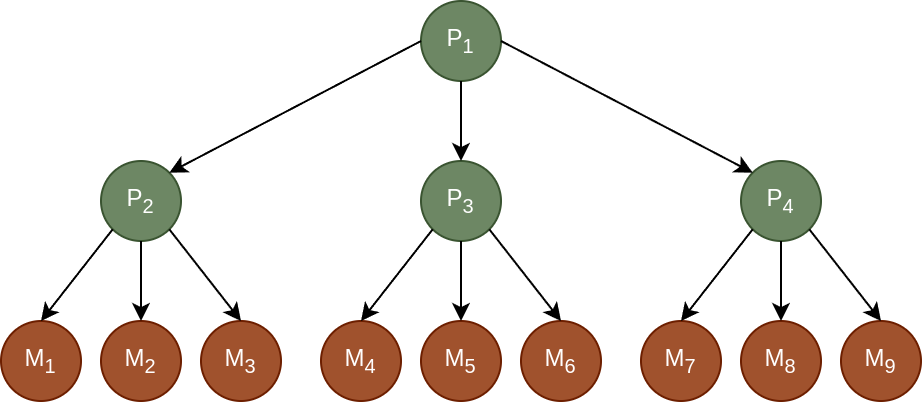
\includegraphics[scale=0.6]{../images/experiment0_topology.png}
	\caption{Experiment 0 - topology}
    \label{fig:experiment0_topology}
\end{figure}

While most of the hyperparameters were transferred from the tuning process directly to the experiments, some of them were scaled. The motivation behind this was to test as many hyperparameter configurations as possible in a limited time, and the hyperparameters which affect complexity the most were scaled down. Table \ref{tab:hyper_scale_population} shows how the population size was scaled, and the table \ref{tab:hyper_scale_evaluations} shows how the number of evaluations was scaled. In the second table, the notation $x/y$ means the following - the loop in the scheduling meta algorithm has $x$ iterations, while the inner optimization algorithm has $y$ evaluations of the evaluation function for the genotype. The goal here was to try to find a good ratio between these two values, while keeping the total number of evaluations of the evaluation function constant.

\begin{table}[!htbp]
    \begin{center}
        \begin{tabular}{|l|l|} 
         \hline
            Old value & New value \\ [0.5ex] \hline\hline
            5 & 50 \\
            \hline
            10 & 100 \\
            \hline
            15 & 150 \\
            \hline
            20 & 200 \\
            \hline
        \end{tabular}
    \end{center}
    \caption{Hyperparameter values - scaling population size}
\label{tab:hyper_scale_population}
\end{table}

\begin{table}[!htbp]
    \begin{center}
        \begin{tabular}{|l|l|} 
         \hline
            Old values & New values \\ [0.5ex] \hline\hline
            10/100 & 50/1000 \\
            \hline
            20/50 & 100/500 \\
            \hline
            40/25 & 200/250 \\
            \hline
            50/20 & 500/100 \\
            \hline
        \end{tabular}
    \end{center}
    \caption{Hyperparameter values - scaling number of evaluations}
\label{tab:hyper_scale_evaluations}
\end{table}

The hyperparameters were tuned for each algorithm separately. This could not be solved using an exhaustive method such as the grid search, as there are too many possible hyperparameter configurations for each algorithm. Instead, the problem was framed as an optimization problem, and the algorithm which was used for optimization was SSGA. A similar approach, used for tuning hyperparameters for machine learning models, can be found in \citep{hyperopti}.

The genotype for this problem was the mapping from hyperparameters to their values. The evaluation function would take these hyperparameters and try to solve the problem of creating a good online scheduling system. In other words, the evaluation function was the execution of the scheduling meta algorithm. The creation operator would generate a random value for each hyperparameter. The combination operator would, for each hyperparameter, randomly choose one of the two parents and copy its value for the hyperparameter. The perturbation operator would randomly select some hyperparameters and change their values. The hyperparameters of the SSGA used for tuning hyperparameters were the following - population size was $10$, number of evaluations of the evaluation function was $200$, and the perturbation rate was $0.2$.

Results of the hyperparameter tuning for online scheduling algorithms are shown in the following tables - NN in table \ref{tab:hyper_nn_results}, 
TBGP in table \ref{tab:hyper_tbgp_results}, CGP in table \ref{tab:hyper_cgp_results}, GBGP in table \ref{tab:hyper_gbgp_results}, SBGP in table \ref{tab:hyper_sbgp_results}, LGP in table \ref{tab:hyper_lgp_results}, MEP in table \ref{tab:hyper_mep_results}, GEP in table \ref{tab:hyper_gep_results}, GE in table \ref{tab:hyper_ge_results} and SGE in table \ref{tab:hyper_sge_results}.

\begin{table}[!htbp]
    \centering
    \resizebox{\textwidth}{!}{
        \begin{tabular}{|l|l|l|l|l|l|l|l|l|l|l|l|}
        \hline
        Hyperparameter & Value \\ [0.5ex] \hline\hline
        cluster combination operator granularity & fine \\
        \hline
        topology partitioner scheme & k true random \\
        \hline
        random path topology enumerator change element chance & 0.6 \\
        \hline
        optimization algorithm & SIA \\
        \hline
        SSGA population size & 5 \\
        \hline
        SSGA evaluations in inner algorithm & 100 \\
        \hline
        GGA population size & 15 \\
        \hline
        GGA evaluations in inner algorithm & 100 \\
        \hline
        GGA worst unit coefficient & 0.1 \\
        \hline
        ES population size & 5 \\
        \hline
        ES evaluations in inner algorithm & 20 \\
        \hline
        ES new units per generation percentage & 0.5 \\
        \hline
        SIA population size & 15 \\
        \hline
        SIA evaluations in inner algorithm & 20 \\
        \hline
        SIA number of clones per individual & 5 \\
        \hline
        CLONALG population size & 15 \\
        \hline
        CLONALG evaluations in inner algorithm & 25 \\
        \hline
        CLONALG $\beta$ & 0.1 \\
        \hline
        CLONALG $\gamma$ & 0.2 \\
        \hline
        CLONALG $\lambda$ & 8 \\
        \hline
        creation $\sigma$ & 0.001 \\
        \hline
        perturbation $\sigma$ & 0.01 \\
        \hline
        activation function & sigmoid \\
        \hline
        hidden layers & $5$ \\
        \hline
        \end{tabular}
    }
    \caption{Hyperparameter tuning results - NN}
    \label{tab:hyper_nn_results}
\end{table}

\begin{table}[!htbp]
    \centering
    \resizebox{\textwidth}{!}{
        \begin{tabular}{|l|l|l|l|l|l|l|l|l|l|l|l|}
        \hline
        Hyperparameter & Value \\ [0.5ex] \hline\hline
        cluster combination operator granularity & fine \\
        \hline
        topology partitioner scheme & k true random \\
        \hline
        random path topology enumerator change element chance & 0.5 \\
        \hline
        optimization algorithm & SSGA \\
        \hline
        SSGA population size & 20 \\
        \hline
        SSGA evaluations in inner algorithm & 20 \\
        \hline
        GGA population size & 10 \\
        \hline
        GGA evaluations in inner algorithm & 20 \\
        \hline
        GGA worst unit coefficient & 0.5 \\
        \hline
        ES population size & 20 \\
        \hline
        ES evaluations in inner algorithm & 25 \\
        \hline
        ES new units per generation percentage & 0.15 \\
        \hline
        SIA population size & 10 \\
        \hline
        SIA evaluations in inner algorithm & 25 \\
        \hline
        SIA number of clones per individual & 4 \\
        \hline
        CLONALG population size & 20 \\
        \hline
        CLONALG evaluations in inner algorithm & 20 \\
        \hline
        CLONALG $\beta$ & 0.5 \\
        \hline
        CLONALG $\gamma$ & 0.15\\
        \hline
        CLONALG $\lambda$ & 10 \\
        \hline
        maximum height & 10 \\
        \hline
        constant leaf chance & 0.05 \\
        \hline
        parameter leaf chance & 0.3 \\
        \hline
        \end{tabular}
    }
    \caption{Hyperparameter tuning results - TBGP}
    \label{tab:hyper_tbgp_results}
\end{table}

\begin{table}[!htbp]
    \centering
    \resizebox{\textwidth}{!}{
        \begin{tabular}{|l|l|l|l|l|l|l|l|l|l|l|l|}
        \hline
        Hyperparameter & Value \\ [0.5ex] \hline\hline
        cluster combination operator granularity & fine \\
        \hline
        topology partitioner scheme & all \\
        \hline
        random path topology enumerator change element chance & 0.6 \\
        \hline
        optimization algorithm & SSGA \\
        \hline
        SSGA population size & 10 \\
        \hline
        SSGA evaluations in inner algorithm & 100 \\
        \hline
        GGA population size & 15 \\
        \hline
        GGA evaluations in inner algorithm & 20 \\
        \hline
        GGA worst unit coefficient & 0.2 \\
        \hline
        ES population size & 5 \\
        \hline
        ES evaluations in inner algorithm & 100 \\
        \hline
        ES new units per generation percentage & 0.4 \\
        \hline
        SIA population size & 5 \\
        \hline
        SIA evaluations in inner algorithm & 25 \\
        \hline
        SIA number of clones per individual & 2 \\
        \hline
        CLONALG population size & 15 \\
        \hline
        CLONALG evaluations in inner algorithm & 50 \\
        \hline
        CLONALG $\beta$ & 0.3 \\
        \hline
        CLONALG $\gamma$ & 0.1 \\
        \hline
        CLONALG $\lambda$ & 10 \\
        \hline
        number of rows & 15 \\
        \hline
        number of columns & 15 \\
        \hline
        perturbation rate & 0.05 \\
        \hline
        \end{tabular}
    }
    \caption{Hyperparameter tuning results - CGP}
    \label{tab:hyper_cgp_results}
\end{table}

\begin{table}[!htbp]
    \centering
    \resizebox{\textwidth}{!}{
        \begin{tabular}{|l|l|l|l|l|l|l|l|l|l|l|l|}
        \hline
        Hyperparameter & Value \\ [0.5ex] \hline\hline
        cluster combination operator granularity & fine \\
        \hline
        topology partitioner scheme & random path \\
        \hline
        random path topology enumerator change element chance & 0.8 \\
        \hline
        optimization algorithm & SSGA \\
        \hline
        SSGA population size & 15 \\
        \hline
        SSGA evaluations in inner algorithm & 50 \\
        \hline
        GGA population size & 10 \\
        \hline
        GGA evaluations in inner algorithm & 20 \\
        \hline
        GGA worst unit coefficient & 0.2 \\
        \hline
        ES population size & 15 \\
        \hline
        ES evaluations in inner algorithm & 20 \\
        \hline
        ES new units per generation percentage & 0.05 \\
        \hline
        SIA population size & 5 \\
        \hline
        SIA evaluations in inner algorithm & 25 \\
        \hline
        SIA number of clones per individual & 2 \\
        \hline
        CLONALG population size & 15 \\
        \hline
        CLONALG evaluations in inner algorithm & 25 \\
        \hline
        CLONALG $\beta$ & 0.2 \\
        \hline
        CLONALG $\gamma$ & 0.1 \\
        \hline
        CLONALG $\lambda$ & 3 \\
        \hline
        maximum number of nodes & 300 \\
        \hline
        perturbation rate & 0.2 \\
        \hline
        maximum nodes to delete & 1 \\
        \hline
        maximum nodes to insert & 4 \\
        \hline
        maximum nodes in crossover & 10 \\
        \hline
        exchange branch in crossover chance & 0.6 \\
        \hline
        \end{tabular}
    }
    \caption{Hyperparameter tuning results - GBGP}
    \label{tab:hyper_gbgp_results}
\end{table}

\begin{table}[!htbp]
    \centering
    \resizebox{\textwidth}{!}{
        \begin{tabular}{|l|l|l|l|l|l|l|l|l|l|l|l|}
        \hline
        Hyperparameter & Value \\ [0.5ex] \hline\hline
        cluster combination operator granularity & coarse \\
        \hline
        topology partitioner scheme & random path \\
        \hline
        random path topology enumerator change element chance & 0.9 \\
        \hline
        optimization algorithm & ES \\
        \hline
        SSGA population size & 20 \\
        \hline
        SSGA evaluations in inner algorithm & 20 \\
        \hline
        GGA population size & 20 \\
        \hline
        GGA evaluations in inner algorithm & 100 \\
        \hline
        GGA worst unit coefficient & 0.5 \\
        \hline
        ES population size & 20 \\
        \hline
        ES evaluations in inner algorithm & 50 \\
        \hline
        ES new units per generation percentage & 0.3 \\
        \hline
        SIA population size & 5 \\
        \hline
        SIA evaluations in inner algorithm & 25 \\
        \hline
        SIA number of clones per individual & 3 \\
        \hline
        CLONALG population size & 10 \\
        \hline
        CLONALG evaluations in inner algorithm & 100 \\
        \hline
        CLONALG $\beta$ & 0.1 \\
        \hline
        CLONALG $\gamma$ & 0.15 \\
        \hline
        CLONALG $\lambda$ & 5 \\
        \hline
        number of instructions & 200 \\
        \hline
        creation chance of NOP & 0.3 \\
        \hline
        perturbation chance of NOP & 0.2 \\
        \hline
        PUSH constant share & 0.1 \\
        \hline
        PUSH param share & 0.3 \\
        \hline
        perturbation rate & 0.3 \\
        \hline
        \end{tabular}
    }
    \caption{Hyperparameter tuning results - SBGP}
    \label{tab:hyper_sbgp_results}
\end{table}

\begin{table}[!htbp]
    \centering
    \resizebox{\textwidth}{!}{
        \begin{tabular}{|l|l|l|l|l|l|l|l|l|l|l|l|}
        \hline
        Hyperparameter & Value \\ [0.5ex] \hline\hline
        cluster combination operator granularity & fine \\
        \hline
        topology partitioner scheme & random path \\
        \hline
        random path topology enumerator change element chance & 0.9 \\
        \hline
        optimization algorithm & ES \\
        \hline
        SSGA population size & 15 \\
        \hline
        SSGA evaluations in inner algorithm & 100 \\
        \hline
        GGA population size & 15 \\
        \hline
        GGA evaluations in inner algorithm & 50 \\
        \hline
        GGA worst unit coefficient & 0.1 \\
        \hline
        ES population size & 5 \\
        \hline
        ES evaluations in inner algorithm & 20 \\
        \hline
        ES new units per generation percentage & 0.3 \\
        \hline
        SIA population size & 10 \\
        \hline
        SIA evaluations in inner algorithm & 100 \\
        \hline
        SIA number of clones per individual & 5 \\
        \hline
        CLONALG population size & 20 \\
        \hline
        CLONALG evaluations in inner algorithm & 25 \\
        \hline
        CLONALG $\beta$ & 0.3 \\
        \hline
        CLONALG $\gamma$ & 0.2 \\
        \hline
        CLONALG $\lambda$ & 5 \\
        \hline
        register initialization strategy & singular \\
        \hline
        number of registers & 10 \\
        \hline
        number of instructions & 100 \\
        \hline
        creation chance of NOP & 0.3 \\
        \hline
        perturbation chance of NOP & 0.4 \\
        \hline
        perturbation rate & 0.05 \\
        \hline
        \end{tabular}
    }
    \caption{Hyperparameter tuning results - LGP}
    \label{tab:hyper_lgp_results}
\end{table}

\begin{table}[!htbp]
    \centering
    \resizebox{\textwidth}{!}{
        \begin{tabular}{|l|l|l|l|l|l|l|l|l|l|l|l|}
        \hline
        Hyperparameter & Value \\ [0.5ex] \hline\hline
        cluster combination operator granularity & fine \\
        \hline
        topology partitioner scheme & k fair random \\
        \hline
        random path topology enumerator change element chance & 0.6 \\
        \hline
        optimization algorithm & ES \\
        \hline
        SSGA population size & 20 \\
        \hline
        SSGA evaluations in inner algorithm & 50 \\
        \hline
        GGA population size & 5 \\
        \hline
        GGA evaluations in inner algorithm & 100 \\
        \hline
        GGA worst unit coefficient & 0.2 \\
        \hline
        ES population size & 5 \\
        \hline
        ES evaluations in inner algorithm & 25 \\
        \hline
        ES new units per generation percentage & 0.05 \\
        \hline
        SIA population size & 20 \\
        \hline
        SIA evaluations in inner algorithm & 100 \\
        \hline
        SIA number of clones per individual & 4 \\
        \hline
        CLONALG population size & 10 \\
        \hline
        CLONALG evaluations in inner algorithm & 50 \\
        \hline
        CLONALG $\beta$ & 0.3 \\
        \hline
        CLONALG $\gamma$ & 0.05 \\
        \hline
        CLONALG $\lambda$ & 5 \\
        \hline
        number of instructions & 150 \\
        \hline
        perturbation rate & 0.05 \\
        \hline
        \end{tabular}
    }
    \caption{Hyperparameter tuning results - MEP}
    \label{tab:hyper_mep_results}
\end{table}

\begin{table}[!htbp]
    \centering
    \resizebox{\textwidth}{!}{
        \begin{tabular}{|l|l|l|l|l|l|l|l|l|l|l|l|}
        \hline
        Hyperparameter & Value \\ [0.5ex] \hline\hline
        cluster combination operator granularity & fine \\
        \hline
        topology partitioner scheme & k true random \\
        \hline
        random path topology enumerator change element chance & 0.5\\
        \hline
        optimization algorithm & GGA \\
        \hline
        SSGA population size & 10 \\
        \hline
        SSGA evaluations in inner algorithm & 100 \\
        \hline
        GGA population size & 10 \\
        \hline
        GGA evaluations in inner algorithm & 50 \\
        \hline
        GGA worst unit coefficient & 0.5 \\
        \hline
        ES population size & 15 \\
        \hline
        ES evaluations in inner algorithm & 20 \\
        \hline
        ES new units per generation percentage & 0.5 \\
        \hline
        SIA population size & 20 \\
        \hline
        SIA evaluations in inner algorithm & 25 \\
        \hline
        SIA number of clones per individual & 4 \\
        \hline
        CLONALG population size & 10 \\
        \hline
        CLONALG evaluations in inner algorithm & 100 \\
        \hline
        CLONALG $\beta$ & 0.3 \\
        \hline
        CLONALG $\gamma$ & 0.1 \\
        \hline
        CLONALG $\lambda$ & 10 \\
        \hline
        head size & 30 \\
        \hline
        tail chance of parameter & 0.9 \\
        \hline
        perturbation rate & 0.3 \\
        \hline
        chance of transposition & 0.2 \\
        \hline
        maximum length of transposition & 20 \\
        \hline
        \end{tabular}
    }
    \caption{Hyperparameter tuning results - GEP}
    \label{tab:hyper_gep_results}
\end{table}

\begin{table}[!htbp]
    \centering
    \resizebox{\textwidth}{!}{
        \begin{tabular}{|l|l|l|l|l|l|l|l|l|l|l|l|}
        \hline
        Hyperparameter & Value \\ [0.5ex] \hline\hline
        cluster combination operator granularity & caorse \\
        \hline
        topology partitioner scheme & k fair random \\
        \hline
        random path topology enumerator change element chance & 0.6 \\
        \hline
        optimization algorithm & CLONALG \\
        \hline
        SSGA population size & 5 \\
        \hline
        SSGA evaluations in inner algorithm & 50 \\
        \hline
        GGA population size & 20 \\
        \hline
        GGA evaluations in inner algorithm & 50 \\
        \hline
        GGA worst unit coefficient & 0.1 \\
        \hline
        ES population size & 15 \\
        \hline
        ES evaluations in inner algorithm & 100 \\
        \hline
        ES new units per generation percentage & 0.2 \\
        \hline
        SIA population size & 5 \\
        \hline
        SIA evaluations in inner algorithm & 100\\
        \hline
        SIA number of clones per individual & 5 \\
        \hline
        CLONALG population size & 10 \\
        \hline
        CLONALG evaluations in inner algorithm & 20 \\
        \hline
        CLONALG $\beta$ & 0.5 \\
        \hline
        CLONALG $\gamma$ & 0.2\\
        \hline
        CLONALG $\lambda$ & 10 \\
        \hline
        number of codons & 300 \\
        \hline
        maximum number of wrappings & 2 \\
        \hline
        perturbation rate & 0.1 \\
        \hline
        \end{tabular}
    }
    \caption{Hyperparameter tuning results - GE}
    \label{tab:hyper_ge_results}
\end{table}

\begin{table}[!htbp]
    \centering
    \resizebox{\textwidth}{!}{
        \begin{tabular}{|l|l|l|l|l|l|l|l|l|l|l|l|}
        \hline
        Hyperparameter & Value \\ [0.5ex] \hline\hline
        cluster combination operator granularity & fine \\
        \hline
        topology partitioner scheme & k fair random \\
        \hline
        random path topology enumerator change element chance & 0.5 \\
        \hline
        optimization algorithm & SSGA \\
        \hline
        SSGA population size & 5 \\
        \hline
        SSGA evaluations in inner algorithm & 50 \\
        \hline
        GGA population size & 5 \\
        \hline
        GGA evaluations in inner algorithm & 25 \\
        \hline
        GGA worst unit coefficient & 0.2 \\
        \hline
        ES population size & 15 \\
        \hline
        ES evaluations in inner algorithm & 20 \\
        \hline
        ES new units per generation percentage & 0.1 \\
        \hline
        SIA population size & 10 \\
        \hline
        SIA evaluations in inner algorithm & 25\\
        \hline
        SIA number of clones per individual & 4 \\
        \hline
        CLONALG population size & 5 \\
        \hline
        CLONALG evaluations in inner algorithm & 25 \\
        \hline
        CLONALG $\beta$ & 0.1 \\
        \hline
        CLONALG $\gamma$ & 0.15\\
        \hline
        CLONALG $\lambda$ & 8 \\
        \hline
        maximum depth & 4 \\
        \hline
        perturbation rate & 0.2 \\
        \hline
        \end{tabular}
    }
    \caption{Hyperparameter tuning results - SGE}
    \label{tab:hyper_sge_results}
\end{table}

The results of the hyperparameter tuning process are fairly interesting. Most of the algorithms (8 out of 10) preferred the fine granularity combination operator. As for the topology partitioner schemes, one algorithm found the \textit{all} partitioner scheme to be the best, three algorithms found the \textit{random path} scheme, three found the \textit{k fair random} scheme, and three found the \textit{k true random} scheme. As for the optimization algorithm, four algorithms preferred SSGA, one preferred GGA, three preferred ES, one preferred SIA and one preferred CLONALG.
\section{Experiments}
\label{sec:experiments}

In this chapter, we will describe the experiments which were used to evaluate online scheduling systems. Each experiment was run for each online scheduling algorithm. Also, each experiment was repeated $10$ times, to be able to draw statistically significant conclusions.

The idea behind these experiments was to create a simple but diverse set of case studies with different behaviors and event types.

\subsection{Experiment 1}

The topology for the first experiment is shown in figure \ref{fig:experiment1_topology}. In this experiment, machines would occasionally have breakdowns. There were two types of jobs. Jobs of the first type generally had lower weights, but they could be preempted, while jobs of the second type generally had higher weights, but they could not be preempted. In the train job sequence, there were a total of $200$ jobs, $100$ of each type. In the test job sequence, there were a total of $600$ jobs, $300$ of each type.

\begin{figure}[!htbp]
	\centering
	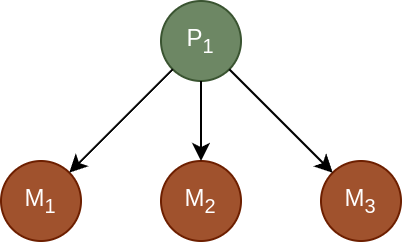
\includegraphics[scale=0.6]{../images/experiment1_topology.png}
	\caption{Experiment 1 - topology}
    \label{fig:experiment1_topology}
\end{figure}

\subsection{Experiment 2}

The topology for the second experiment is shown in figure \ref{fig:experiment2_topology}. In this experiment, there were three job types, and preemptions were allowed for all of them. The batch processing limit of every job type on the machines was $3$. In the train job sequence, there were a total of $240$ jobs, $80$ of each type. In the test job sequence, there were a total of $600$ jobs, $200$ of each type.

\begin{figure}[!htbp]
	\centering
	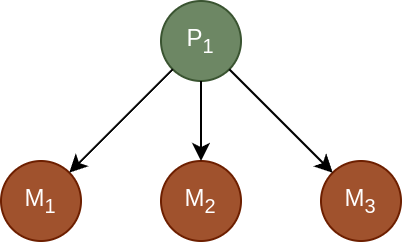
\includegraphics[scale=0.6]{../images/experiment2_topology.png}
	\caption{Experiment 2 - topology}
    \label{fig:experiment2_topology}
\end{figure}

\subsection{Experiment 3}

The topology for the third experiment is shown in figure \ref{fig:experiment3_topology}. In this experiment, every machine had a buffer of size $3$, and some jobs had prerequisites in regards to jobs which entered the system before. In each parallel group, there were two fast machines, and one which was slower in processing jobs. In the train job sequence, there were a total of $200$ jobs. In the test job sequence, there were a total of $500$ jobs.

\begin{figure}[!htbp]
	\centering
	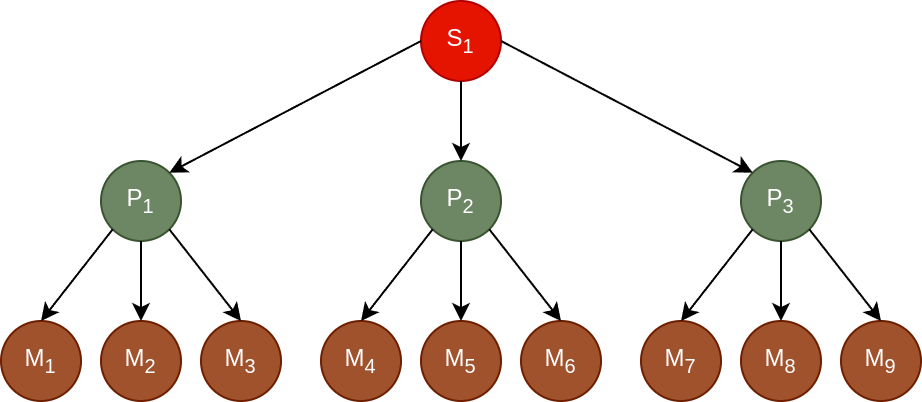
\includegraphics[scale=0.6]{../images/experiment3_topology.png}
	\caption{Experiment 3 - topology}
    \label{fig:experiment3_topology}
\end{figure}

\subsection{Experiment 4}

The topology for the fourth experiment is shown in figure \ref{fig:experiment4_topology}. In this experiment, a total of $3$ jobs could be processed in a batch. Also, there was a setup on every machine between processing two jobs, which took half the time that the processing of a job on a machine took. In the train job sequence, there were a total of $200$ jobs. In the test job sequence, there were a total of $500$ jobs.

\begin{figure}[!htbp]
	\centering
	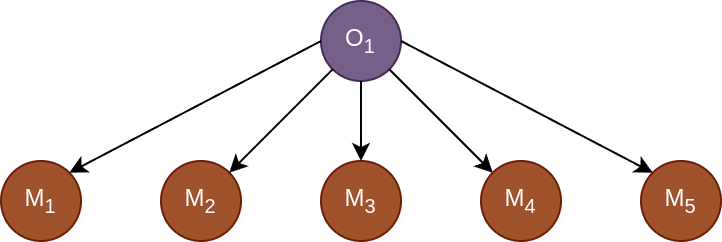
\includegraphics[scale=0.6]{../images/experiment4_topology.png}
	\caption{Experiment 4 - topology}
    \label{fig:experiment4_topology}
\end{figure}

\subsection{Experiment 5}

The topology for the fifth experiment is shown in figure \ref{fig:experiment5_topology}. In this experiment, jobs could be preempted from machines, and there was a setup on every machine between processing two jobs, which took half the time that the processing of a job on a machine took, the same as the previous experiment. In the train job sequence, there were a total of $200$ jobs. In the test job sequence, there were a total of $500$ jobs.

\begin{figure}[!htbp]
	\centering
	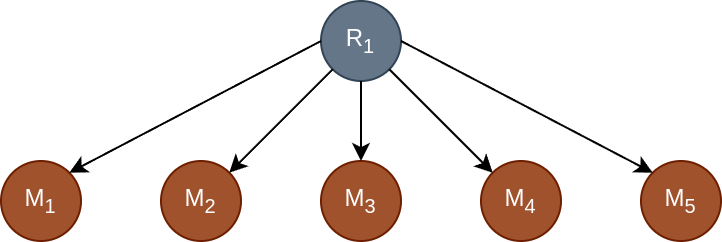
\includegraphics[scale=0.6]{../images/experiment5_topology.png}
	\caption{Experiment 5 - topology}
    \label{fig:experiment5_topology}
\end{figure}
\section{Results}

\chapter{Conclusion}
\label{sec:conclusion}
In this thesis, we have introduced the hierarchical topology representation for solving scheduling problems. We have described how to represent scheduling systems, how to model their complex behaviors, how to evaluate them, and how to optimize them both in an offline and an online setting. Through a series of experiments, we have demonstrated that this representation can be used to solve online scheduling problems across a variety of system and event characteristics, deeming the representation both effective and versatile.

There are several directions in which future research could go. One of them is exploring different feature sets in online scheduling algorithms, as discussed in \ref{sec:online_scheduling_limitations}. Another direction could be to explore different genotype operators for the algorithms which performed the best in our experiments, to further optimize these representations for online scheduling problems. Finally, since all the case studies in this thesis were artificial, it would be interesting to solve real problems using the concepts presented in this thesis. The hierarchical topology representation proved to be highly effective for solving online scheduling problems in a somewhat idealized environment, which indicates that it potentially could be used for solving problems in real environments as well.

\bibliography{literatura}
\bibliographystyle{fer}

\listoffigures

\listoftables

\listofalgorithms
\addcontentsline{toc}{chapter}{List of Algorithms}

\begin{sazetak}
In this thesis, a novel approach to solving scheduling problems is presented. The model of scheduling which was used was the model of machines and jobs, in which a system consists of several machines and their connections, a certain number of jobs needs to be processed in the system, and the scheduler needs to decide, at each moment, which job is being processed on which machine, in order to optimize some criteria. A model for representing machine topologies is introduced. This model is extended with an events model, which supports complex behaviors such as preemptions, breakdowns, setups, prerequisites, buffers of a limited size and batch processing. Evaluation and optimization of such systems in both an offline and an online setting is presented. Through a series of case studies, containing problems of different configurations and behaviors, it is demonstrated that this model can be used to successfully solve online scheduling problems. The solution was achieved using hyperheuristics, where the goal is not to effectively solve a problem, instead the goal is to find an effective method for solving a problem.

\kljucnerijeci{scheduling, online scheduling, optimization, metaheuristics, hyperheuristics, evolutionary computing, genetic programming}
\end{sazetak}

\newpage

\engtitle{Optimizacija hiperheuristika za probleme raspoređivanja na zahtjev}
\begin{abstract}
U ovom je radu predstavljen novi pristup rješavanju problema raspoređivanja. Model raspoređivanja koji je korišten je model strojeva i poslova, gdje se sustav sastoji od nekoliko strojeva i njihovih međusobnih veza, određen broj poslova treba biti obrađen u sustavu, i cilj raspoređivača je da, u svakom trenutku, odredi koji posao se izvodi na kojem stroju, kako bi optimirao neke kriterije. Model za reprezentaciju topologija strojeva je predstavljen. Ovaj model je proširen s model događaja, koji podržava složena ponašanja poput prekida izvođenja poslova, kvarova strojeva, izmjene konteksta između poslova, preduvjeta za izvođenje, redova čekanja s ograničenom veličinom i grupnim izvođenjem poslova. Objašnjeni su evaluacija i optimizacija takvih sustava u predeterminiranom načinu rada, i načinu rada na zahtjev. Kroz nekoliko studija slučaja, koje su sadržavale probleme različitih konfiguracija i ponašanja, demonstrirano je da se ovaj model može iskoristiti za uspješno rješavanje problema raspoređivanja na zahtjev. Rješenje je ostvareno korištenjem hiperheuristika, gdje cilj nije efektivno riješiti neki problem, nego je cilj pronaći efektivnu metodu za rješavanje problema.

\keywords{raspoređivanje, raspoređivanje na zahtjev, optimizacija, metaheuristike, hiperheuristike, evolucijsko računarstvo, genetsko programiranje}
\end{abstract}

\end{document}